%==============================================================================
% tento soubor pouzijte jako zaklad
% this file should be used as a base for the thesis
% Autoři / Authors: 2008 Michal Bidlo, 2019 Jaroslav Dytrych
% Kontakt pro dotazy a připomínky: sablona@fit.vutbr.cz
% Contact for questions and comments: sablona@fit.vutbr.cz
%==============================================================================
% kodovani: UTF-8 (zmena prikazem iconv, recode nebo cstocs)
% encoding: UTF-8 (you can change it by command iconv, recode or cstocs)
%------------------------------------------------------------------------------
% zpracování / processing: make, make pdf, make clean
%==============================================================================
% Soubory, které je nutné upravit nebo smazat: / Files which have to be edited or deleted:
%   projekt-20-literatura-bibliography.bib - literatura / bibliography
%   projekt-01-kapitoly-chapters.tex - obsah práce / the thesis content
%   projekt-01-kapitoly-chapters-en.tex - obsah práce v angličtině / the thesis content in English
%   projekt-30-prilohy-appendices.tex - přílohy / appendices
%   projekt-30-prilohy-appendices-en.tex - přílohy v angličtině / appendices in English
%==============================================================================
%\documentclass[]{fitthesis} % bez zadání - pro začátek práce, aby nebyl problém s překladem
%\documentclass[english]{fitthesis} % without assignment - for the work start to avoid compilation problem
%\documentclass[zadani]{fitthesis} % odevzdani do wisu a/nebo tisk s barevnými odkazy - odkazy jsou barevné
\documentclass[english,zadani]{fitthesis} % for submission to the IS FIT and/or print with color links - links are color
%\documentclass[zadani,print]{fitthesis} % pro černobílý tisk - odkazy jsou černé
%\documentclass[english,zadani,print]{fitthesis} % for the black and white print - links are black
%\documentclass[zadani,cprint]{fitthesis} % pro barevný tisk - odkazy jsou černé, znak VUT barevný
%\documentclass[english,zadani,cprint]{fitthesis} % for the print - links are black, logo is color
% * Je-li práce psaná v anglickém jazyce, je zapotřebí u třídy použít 
%   parametr english následovně:
%   If thesis is written in English, it is necessary to use 
%   parameter english as follows:
%      \documentclass[english]{fitthesis}
% * Je-li práce psaná ve slovenském jazyce, je zapotřebí u třídy použít 
%   parametr slovak následovně:
%   If the work is written in the Slovak language, it is necessary 
%   to use parameter slovak as follows:
%      \documentclass[slovak]{fitthesis}
% * Je-li práce psaná v anglickém jazyce se slovenským abstraktem apod., 
%   je zapotřebí u třídy použít parametry english a enslovak následovně:
%   If the work is written in English with the Slovak abstract, etc., 
%   it is necessary to use parameters english and enslovak as follows:
%      \documentclass[english,enslovak]{fitthesis}

% Základní balíčky jsou dole v souboru šablony fitthesis.cls
% Basic packages are at the bottom of template file fitthesis.cls
% zde můžeme vložit vlastní balíčky / you can place own packages here

% Kompilace po částech (rychlejší, ale v náhledu nemusí být vše aktuální)
% Compilation piecewise (faster, but not all parts in preview will be up-to-date)
% \usepackage{subfiles}

% Nastavení cesty k obrázkům
% Setting of a path to the pictures
%\graphicspath{{obrazky-figures/}{./obrazky-figures/}}
%\graphicspath{{obrazky-figures/}{../obrazky-figures/}}

%---rm---------------
\renewcommand{\rmdefault}{lmr}%zavede Latin Modern Roman jako rm / set Latin Modern Roman as rm
%---sf---------------
\renewcommand{\sfdefault}{qhv}%zavede TeX Gyre Heros jako sf
%---tt------------
\renewcommand{\ttdefault}{lmtt}% zavede Latin Modern tt jako tt

% vypne funkci šablony, která automaticky nahrazuje uvozovky,
% aby nebyly prováděny nevhodné náhrady v popisech API apod.
% disables function of the template which replaces quotation marks
% to avoid unnecessary replacements in the API descriptions etc.
\csdoublequotesoff



\usepackage{url}


% =======================================================================
% balíček "hyperref" vytváří klikací odkazy v pdf, pokud tedy použijeme pdflatex
% problém je, že balíček hyperref musí být uveden jako poslední, takže nemůže
% být v šabloně
% "hyperref" package create clickable links in pdf if you are using pdflatex.
% Problem is that this package have to be introduced as the last one so it 
% can not be placed in the template file.
\ifWis
\ifx\pdfoutput\undefined % nejedeme pod pdflatexem / we are not using pdflatex
\else
  \usepackage{color}
  \usepackage[unicode,colorlinks,hyperindex,plainpages=false,pdftex]{hyperref}
  \definecolor{hrcolor-ref}{RGB}{223,52,30}
  \definecolor{hrcolor-cite}{HTML}{2F8F00}
  \definecolor{hrcolor-urls}{HTML}{092EAB}
  \hypersetup{
	linkcolor=hrcolor-ref,
	citecolor=hrcolor-cite,
	filecolor=magenta,
	urlcolor=hrcolor-urls
  }
  \def\pdfBorderAttrs{/Border [0 0 0] }  % bez okrajů kolem odkazů / without margins around links
  \pdfcompresslevel=9
\fi
\else % pro tisk budou odkazy, na které se dá klikat, černé / for the print clickable links will be black
\ifx\pdfoutput\undefined % nejedeme pod pdflatexem / we are not using pdflatex
\else
  \usepackage{color}
  \usepackage[unicode,colorlinks,hyperindex,plainpages=false,pdftex,urlcolor=black,linkcolor=black,citecolor=black]{hyperref}
  \definecolor{links}{rgb}{0,0,0}
  \definecolor{anchors}{rgb}{0,0,0}
  \def\AnchorColor{anchors}
  \def\LinkColor{links}
  \def\pdfBorderAttrs{/Border [0 0 0] } % bez okrajů kolem odkazů / without margins around links
  \pdfcompresslevel=9
\fi
\fi
% Řešení problému, kdy klikací odkazy na obrázky vedou za obrázek
% This solves the problems with links which leads after the picture
\usepackage[all]{hypcap}

% Informace o práci/projektu / Information about the thesis
%---------------------------------------------------------------------------
\projectinfo{
  %Prace / Thesis
  project={BP},            %typ práce BP/SP/DP/DR  / thesis type (SP = term project)
  year={2023},             % rok odevzdání / year of submission
  date={May 3, 2023},             % datum odevzdání / submission date
  %Nazev prace / thesis title
  title.cs={Klasifikace pomocí neuronových sítí v prostředí Keras},  % název práce v češtině či slovenštině (dle zadání) / thesis title in czech language (according to assignment)
  title.en={Classification with neural networks in the Keras environment}, % název práce v angličtině / thesis title in english
  %title.length={14.5cm}, % nastavení délky bloku s titulkem pro úpravu zalomení řádku (lze definovat zde nebo níže) / setting the length of a block with a thesis title for adjusting a line break (can be defined here or below)
  %sectitle.length={14.5cm}, % nastavení délky bloku s druhým titulkem pro úpravu zalomení řádku (lze definovat zde nebo níže) / setting the length of a block with a second thesis title for adjusting a line break (can be defined here or below)
  %dectitle.length={14.5cm}, % nastavení délky bloku s titulkem nad prohlášením pro úpravu zalomení řádku (lze definovat zde nebo níže) / setting the length of a block with a thesis title above declaration for adjusting a line break (can be defined here or below)
  %Autor / Author
  author.name={Michal},   % jméno autora / author name
  author.surname={Pyšík},   % příjmení autora / author surname 
  %author.title.p={Bc.}, % titul před jménem (nepovinné) / title before the name (optional)
  %author.title.a={Ph.D.}, % titul za jménem (nepovinné) / title after the name (optional)
  %Ustav / Department
  department={UIFS}, % doplňte příslušnou zkratku dle ústavu na zadání: UPSY/UIFS/UITS/UPGM / fill in appropriate abbreviation of the department according to assignment: UPSY/UIFS/UITS/UPGM
  % Školitel / supervisor
  supervisor.name={Vladimír},   % jméno školitele / supervisor name 
  supervisor.surname={Bartík},   % příjmení školitele / supervisor surname
  supervisor.title.p={Ing.},   %titul před jménem (nepovinné) / title before the name (optional)
  supervisor.title.a={Ph.D.},    %titul za jménem (nepovinné) / title after the name (optional)
  % Klíčová slova / keywords
  keywords.cs={Keras, Tensorflow, klasifikace, umělé neuronové sítě,
  typy neuronových sítí, topologie neuronových sítí, porovnání neuronových sítí,
  vícevrstvé perceptrony, konvoluční neuronové sítě, rekurentní neuronové sítě, experimenty
  }, % klíčová slova v českém či slovenském jazyce / keywords in czech or slovak language
  keywords.en={Keras, Tensorflow, classification, artificial neural networks,
  types of neural networks, topologies of neural networks, comparison of neural networks,
  multilayer perceptrons, convolutional neural networks, recurrent neural networks, experiments
  }, % klíčová slova v anglickém jazyce / keywords in english
  %keywords.en={Here, individual keywords separated by commas will be written in English.},
  % Abstrakt / Abstract
  abstract.cs={Tato práce zkoumá problematiku klasifikace pomocí
  umělých neuronových sítí s využitím knihovny Keras,
  poskytující vysokoúrovňové rozhraní pro práci s umělými neuronovými sítěmi v programovacím jazyce Python. Cílem práce je prozkoumat rozsáhlé
  možnosti této knihovny v oblasti klasifikace a porovnat různé typy a topologie umělých neuronových sítí
  formou experimentů na vybraných datasetech,
  což je doplněno jednoduchou experimentální aplikací sloužící především jako rozhraní pro tyto experimenty.}, 
  % abstrakt v českém či slovenském jazyce / abstract in czech or slovak language
  abstract.en={This thesis examines the problematics of classification using
  artificial neural networks within use of the Keras framework,
  a high-level deep learning API for the Python programming language. The aim of the thesis is to discover the
  diverse options Keras has to offer in the field of classification, and to compare different types and topologies
  of artificial neural networks in the form of experiments on selected datasets, complemented
  by a simple experimental application whose main purpose is to provide an interface for these experiments.},
  % abstrakt v anglickém jazyce / abstract in english
  % Prohlášení (u anglicky psané práce anglicky, u slovensky psané práce slovensky) / Declaration (for thesis in english should be in english)
  %declaration={Prohlašuji, že jsem tuto bakalářskou práci vypracoval samostatně pod vedením pana Ing. Vladimíra Bartíka, Ph.D.
%Další informace mi poskytli...
%Uvedl jsem všechny literární prameny, publikace a další zdroje, ze kterých jsem čerpal.},
  declaration={I hereby declare that this Bachelor's thesis was prepared as an original work by the author under the supervision of Mr. Ing. Vladimír Bartík, Ph.D.
  I have listed all the literary sources, publications and other sources, which were used during the preparation of this thesis.},
  % Poděkování (nepovinné, nejlépe v jazyce práce) / Acknowledgement (optional, ideally in the language of the thesis)
  %acknowledgment={V této sekci je možno uvést poděkování vedoucímu práce a těm, kteří poskytli odbornou pomoc
  %(externí zadavatel, konzultant apod.).},
  acknowledgment={I would like to express my gratitude towards my supervisor, Ing. Vladimír Bartík, Ph.D.,
  who was always willing to consult the state of the work with me and whose suggestions helped greatly
  towards reaching the thesis' final state.
  I would also like to thank my family and friends for their continuous support throughout my studies.
  },
  % Rozšířený abstrakt (cca 3 normostrany) - lze definovat zde nebo níže / Extended abstract (approximately 3 standard pages) - can be defined here or below
  extendedabstract={
  Klasifikace je jedním z~nejběžnějších problémů v~oblasti strojového učení. Cílem klasifikačního problému je přiřadit
  jednotlivá vstupní data do předem definovaných kategorií (tříd). To lze provést například použitím umělých neuronových sítí
  (dále jen neuronové sítě),
  které jsou inspirovány biologickými neuronovými sítěmi a~jsou běžně využívány v~mnoha doménách, včetně klasifikace.
  Vzhledem k~tomu, že takové (nejen klasifikační) problémy můžou nabývat mnoha dosti odlišných podob,
  jako je například klasifikace obrázků či mluvené řeči, existuje více specializovaných typů těchto sítí.
  Pro práci s~neuronovými sítěmi v dnešní době již není třeba znát podrobně jejich vnitřní mechanismy,
  ale lze využít jedno z~vysokoúrovňových rozhraní pro práci s~nimi, kam mimo jiné spadá také knihovna Keras.
  
  Cílem této bakalářské práce je prozkoumat rozsáhlé možnosti prostředí Keras v~oblasti klasifikace pomocí neuronových sítí
  a~porovnat vlastnosti různých typů a~topologií neuronových sítí formou experimentů na vybraných datasetech.
  Jelikož se různé typy neuronových sítí v~mnoha ohledech výrazně liší, není jejich porovnání snadným problémem.
  Z~těchto důvodů byly vybrány tři odlišné datasety, kdy každý dataset svou charakteristikou odpovídá jednomu ze tří
  hlavních druhů neuronových sítí (vícevrstvý perceptron, konvoluční neuronová síť, rekurentní neuronová síť).
  Pro každý ze tří experimentů byly individuálně vytvořeny čtyři neuronové sítě,
  a~to nejen jedna od každého ze tří typů, ale dále ještě jedna odpovídající svým typem charakteristice daného experimentu,
  za účelem porovnání vícera topologií neuronových sítí. Jako rozhraní pro průběh experimentů slouží jednoduchá experimentální
  aplikace napsána v~programovacím jazyce Python s~využitím knihovny Keras, která zahrnuje mnoho funkcí umožňující důkladně
  monitorovat průběh trénování, a~vyhodnocení (nejen) daných neuronových sítí.
  
  Práce začíná úvodem do problematiky klasifikace představením klíčových pojmů, metrik pro měření výkonnosti klasifikačního modelu,
  a~stručným popisem vybraných alternativních klasifikačních algoritmů. Poté jsou představeny umělé neuronové sítě,
  a~to způsobem vhodným
  i~pro čtenáře neznalého v~dané problematice. Tato část je postupně rozvinuta od nejjednodušších stavebních bloků (neuronů)
  až po rozdíly mezi jednotlivými typy neuronových sítí. Dále následuje kapitola věnující se samotné knihovně Keras,
  která je strukturována chronologicky v~souladu s~vytvářením vlastních klasifikačních modelů. U~každého kroku
  jsou popsány odlišné přístupy a~možnosti, které zde Keras nabízí.
  
  Samotné experimenty začínají jejich přípravou, včetně analýzy jednotlivých datasetů, způsobů interpretace odlišných druhů dat
  jednotlivými typy neuronových sítí, a~výběrem architektur použitých sítí. Zde jsou také odůvodněny různá rozhodnutí,
  která jsou klíčová pro průběh experimentů a~jejich přínos. Po stručném popisu návrhu a~implementace experimentální
  aplikace následuje popis průběhu jednotlivých experimentů, především formou popisu grafů vygenerovaných pomocí experimentání
  aplikace, a~jejich vyhodnocení formou jednotlivých závěrů a~konečným shrnutím. Ačkoli by nebylo vhodné dělat příliš
  vážné závěry čistě na základě relativní výkonnosti jednotlivých modelů, jelikož může být silně ovlivněna příliš mnoha faktory,
  byly demonstrovány jednotlivé vlastnosti odlišných typů neuronových sítí a~jejich využitelnost v~oblastech
  neobvyklých pro daný typ sítě. V rámci experimentů byly také nalezeny určité neočekávané poznatky.
  Po vyvození závěrů byly dále navrženy vhodné možnosti pro rozšíření této práce, především
  v~kontextu moderních architektur neuronových sítí a~aktuálních trendů v~této oblasti.
  },
  %extabstract.odd={true}, % Začít rozšířený abstrakt na liché stránce? / Should extended abstract start on the odd page?
  faculty={FIT}, % FIT/FEKT/FSI/FA/FCH/FP/FAST/FAVU/USI/DEF
  faculty.cs={Fakulta informačních technologií}, % Fakulta v češtině - pro využití této položky výše zvolte fakultu DEF / Faculty in Czech - for use of this entry select DEF above
  faculty.en={Faculty of Information Technology}, % Fakulta v angličtině - pro využití této položky výše zvolte fakultu DEF / Faculty in English - for use of this entry select DEF above
  department.cs={Ústav matematiky}, % Ústav v češtině - pro využití této položky výše zvolte ústav DEF nebo jej zakomentujte / Department in Czech - for use of this entry select DEF above or comment it out
  department.en={Institute of Mathematics} % Ústav v angličtině - pro využití této položky výše zvolte ústav DEF nebo jej zakomentujte / Department in English - for use of this entry select DEF above or comment it out
}

% Rozšířený abstrakt (cca 3 normostrany) - lze definovat zde nebo výše / Extended abstract (approximately 3 standard pages) - can be defined here or above
%\extendedabstract{Do tohoto odstavce bude zapsán výtah (abstrakt) práce v českém (slovenském) jazyce.}
% Začít rozšířený abstrakt na liché stránce? / Should extended abstract start on the odd page?
%\extabstractodd{true}

% nastavení délky bloku s titulkem pro úpravu zalomení řádku - lze definovat zde nebo výše / setting the length of a block with a thesis title for adjusting a line break - can be defined here or above
%\titlelength{14.5cm}
% nastavení délky bloku s druhým titulkem pro úpravu zalomení řádku - lze definovat zde nebo výše / setting the length of a block with a second thesis title for adjusting a line break - can be defined here or above
%\sectitlelength{14.5cm}
% nastavení délky bloku s titulkem nad prohlášením pro úpravu zalomení řádku - lze definovat zde nebo výše / setting the length of a block with a thesis title above declaration for adjusting a line break - can be defined here or above
%\dectitlelength{14.5cm}

% řeší první/poslední řádek odstavce na předchozí/následující stránce
% solves first/last row of the paragraph on the previous/next page
\clubpenalty=10000
\widowpenalty=10000

% checklist
\newlist{checklist}{itemize}{1}
\setlist[checklist]{label=$\square$}

% Nechcete-li, aby se u oboustranného tisku roztahovaly mezery pro zaplnění stránky, odkomentujte následující řádek / If you do not want enlarged spacing for filling of the pages in case of duplex printing, uncomment the following line
% \raggedbottom

%%%%%%%%%%%%%%%%%%%%%%%%%%%%%%%%%%%%%%%%%%%%%%%%%%%%%%%%%
%% MOJE PACKAGE A NASTAVENI %%
\usepackage{pgfplots}
\pgfplotsset{compat=newest}
\usepackage{tikz}
\usetikzlibrary{matrix,chains,positioning,decorations.pathreplacing,arrows,fit,backgrounds,intersections,babel}
\usepackage{subcaption}
\usepackage{listofitems} % for \readlist to create arrays
\usepackage[outline]{contour} % glow around text
\contourlength{1.4pt}
%\usepackage[ruled,vlined,linesnumbered,resetcount,algochapter]{algorithm2e}
\usepackage[chapter]{algorithm}
\usepackage{listings}
\lstset{language=Python, morekeywords={tf, keras, layers, regularizers, initializers,
optimizers, losses, metrics, datasets, mnist, callbacks}, basicstyle=\ttfamily}
\usepackage{diagbox}
\usepackage[bottom]{footmisc}


% FIGURE 3.4
\usepackage{xcolor}
\colorlet{myred}{red!80!black}
\colorlet{myblue}{blue!80!black}
\colorlet{mygreen}{green!60!black}
\colorlet{mydarkblue}{blue!40!black}
\tikzstyle{node}=[thick,circle,draw=myblue,minimum size=22,inner sep=0.5,outer sep=0.6]
\tikzstyle{node in}=[node,green!20!black,draw=mygreen!30!black,fill=mygreen!25]
\tikzstyle{node hidden}=[node,blue!20!black,draw=myblue!30!black,fill=myblue!20]
\tikzstyle{node out}=[node,red!20!black,draw=myred!30!black,fill=myred!20]
\tikzstyle{connect}=[thick,mydarkblue] %,line cap=round
\tikzstyle{connect arrow}=[-{Latex[length=4,width=3.5]},thick,mydarkblue,shorten <=0.5,shorten >=1]
\tikzset{ % node styles, numbered for easy mapping with \nstyle
  node 1/.style={node in},
  node 2/.style={node hidden},
  node 3/.style={node out},
}
\def\nstyle{int(\lay<\Nnodlen?min(2,\lay):3)} % map layer number onto 1, 2, or 3


%%%%%%%%%%%%%%%%%%%%%%%%%%%%%%%%%%%%%%%%%%%%%%%%%%%%%%%%

\begin{document}
  % Vysazeni titulnich stran / Typesetting of the title pages
  % ----------------------------------------------
  \maketitle
  % Obsah
  % ----------------------------------------------
  \setlength{\parskip}{0pt}

  \setcounter{tocdepth}{1} % - nechci subsekce v obsahu
  {\hypersetup{hidelinks}\tableofcontents}
  
  % Seznam obrazku a tabulek (pokud prace obsahuje velke mnozstvi obrazku, tak se to hodi)
  % List of figures and list of tables (if the thesis contains a lot of pictures, it is good)
  \ifczech
    \renewcommand\listfigurename{Seznam obrázků}
  \fi
  \ifslovak
    \renewcommand\listfigurename{Zoznam obrázkov}
  \fi
  % {\hypersetup{hidelinks}\listoffigures}
  
  \ifczech
    \renewcommand\listtablename{Seznam tabulek}
  \fi
  \ifslovak
    \renewcommand\listtablename{Zoznam tabuliek}
  \fi
  % {\hypersetup{hidelinks}\listoftables}

  \ifODSAZ
    \setlength{\parskip}{0.5\bigskipamount}
  \else
    \setlength{\parskip}{0pt}
  \fi

  % vynechani stranky v oboustrannem rezimu
  % Skip the page in the two-sided mode
  \iftwoside
    \cleardoublepage
  \fi

  % Text prace / Thesis text
  % ----------------------------------------------
  \ifenglish
    % File containing all chapters.
%=========================================================================

\chapter{Introduction}
\label{introduction}
In recent years, the field of artificial intelligence has seen a significant rise in popularity, thanks to advancements in technology and the availability of large datasets.
One of the most popular and successful computational models in this field are artificial
neural networks, inspired by the function of real biological brains. These models have been widely used
in various applications, whether it be simple ones, like digit classification, or complex natural language
processing applications, like AI assistants.

Classification is a fundamental task in machine learning,
where the goal is to predict the class label of a given input,
by classifying the input object into one of a finite number of classes based on its features.
In this sense, an object is nothing more a set of numerical values, but they do not always represent its features directly.
In the case of, for example,
images or audio files, the features have to be extracted first.
This is usually learned and done by the model itself, at least in the case of deep learning.
Artificial neural networks have proven themselves to be especially helpful when it comes to
complex non-linear tasks, due to their ability to handle complex relationships between variables
and their ability to learn from large amounts of data.
There are many different types of neural networks, each suitable for problems of a different nature.

To start solving problems using neural networks today, there's no longer
a need for learning all the mathematical principles of their internal mechanism.
Any of the high-level deep-learning APIs currently available, which include
the Keras library, can be used instead.
The topic of this thesis revolves around utilization of the Keras library
in the field of classification using neural networks.
The main goals are to introduce neural networks in a way that even a reader inexperienced in the problematics
can understand, to explore Keras' distinct options in the context of classification using neural networks,
and to compare different types and topologies of neural networks through thoughtful experiments.

The theoretical part of the thesis introduces the concepts of classification (chapter \ref{classification})
and artificial neural networks (chapter \ref{artificial-neural-networks}) from the ground up.
Chapter \ref{the-keras-library} then introduces the Keras library in the form of a chronological use case guide.
Finally, the practical part consists of preparation of the experiments in chapter \ref{preparation-of-the-experiments},
brief description of the experimental application (chapter \ref{the-experimental-application}), that serves
as an interface for the experiments, and ends with the course and evaluation of the experiments in chapter
\ref{course-and-evaluation-of-the-experiments}.



\chapter{Classification}
\label{classification}
This chapter is an introduction to the problematics of classification, one of the most common kinds
of tasks in machine learning---a field of study concerned with algorithms that can learn to solve
many different kinds of tasks by learning from data. The goal of a classification
task is to assign discrete class labels to objects from the problem domain, for example
differentiating between pictures of cats and dogs. Classification falls into the category
of supervised learning, since the model learns to predict classes of objects
by training on labeled datasets.
Some other common types of machine learning problems include regression (supervised learning),
which is about predicting a continuous values, and clustering (unsupervised learning),
whose goal is to group instances into unlabeled categories based on their similarity.

Section~\ref{terminology-and-types-of-tasks} explains basic classification
terminology and types, into which can be different classification
tasks divided~\cite{classification-in-machine-learning}, followed by
section~\ref{evaluating-a-models-performance}, which introduces miscellaneous
evaluation metrics for measuring a classification model's performance.
Besides artificial neural networks,
the primary subject of this thesis, explained later in chapter~\ref{artificial-neural-networks},
I considered it appropriate to also mention a few simpler
classification algorithms~\cite{classification-algorithms} in
section~\ref{other-classification-algorithms},
that can sometime be more effective in the cases of simpler problems.





\section{Terminology and types of tasks}
\label{terminology-and-types-of-tasks}
This short section explains some of the technical terms that are crucial to understand before reading further.


\subsection*{Basic terminology}
\label{basic-terminology}
\begin{itemize}
    \item \textbf{Classifier} -- An algorithm used to map objects from the input set of data
    to specific classes. Classifiers can range from simple algorithms all the way
    to deep neural networks consisting of many hidden layers.
    \item \textbf{Model} -- A classification model learns to draw some conclusion
    from the input data given for training, which can be later utilized to predict
    class labels of new data. Simply said, the model consists of the selected classifier
    and the experience gained by training on labeled data.
    \item \textbf{Feature} -- An individual measurable property of a phenomenon. Features
    need to be transformed into numerical representations before being fed to the classifier.
    \item \textbf{Instance} -- A feature vector, an n-dimensional vector of numerical values
    that represent some object. It is referred to as a sample in the context of a dataset.
    Some examples can be a single row in a table of data,
    or a multi-dimensional vector, where the feature values might correspond to the pixels of an image.
    \item \textbf{Dataset} -- A collection of instances (samples), that is a subset of a given feature
    space\footnote{Feature space is the set of all possible values for a chosen set of features from given data.}.
    Datasets are used for training, validating and testing the model.
    \item \textbf{Model training} -- The purpose of training is to build the best mathematical representation
    of the relationship between data features and the target labels. This is done by feeding a labeled
    training dataset to the model, which then adjusts itself to make more accurate predictions,
    by trying to minimize the value of a loss function, which computes the distance
    between the expected output and the model's prediction.
    \item \textbf{Model evaluation} -- Ways to evaluate the performance of the model.
    A quantifiable measure is called a metric.
\end{itemize}


\subsection*{Types of tasks}
\label{types-of-tasks}
\begin{itemize}
    \item \textbf{Binary classification} -- Classification tasks that have only two class labels. Examples include
    predicting whether an email is a spam based on the most occurring words, or distinguishing males
    from females based on their favorite hobbies.
    \item \textbf{Multi-class classification} -- Tasks with more than two class labels. Each instance
    is assigned only one label. A good example may be recognizing the species of the animal
    in a photo of a single animal.
    \item \textbf{Multi-label classification} -- Each instance may be assigned more than one class label,
    including none or all of them.
    For example, classifying which kinds of fruit are contained in images of fruit bowls.
    \item \textbf{Balanced/imbalanced classification} -- The distribution of classes in a training dataset
    may not always be uniform. A very good example is detection of a certain medical condition in patients.
    In these cases, other classification metrics become prioritized over plain accuracy,
    as false detection of the condition in a healthy patient usually leads to less damage
    than misclassifying a sick patient as healthy.
\end{itemize}




\section{Evaluating a model's performance}
\label{evaluating-a-models-performance}
There are many different evaluation metrics that can be used to measure a classification model's
performance~\cite{hossin2015review}.
The simplest and also the most commonly used one is accuracy, which is calculated simply
as the number of correct predictions divided by the sum of all predictions.

All classification metrics are based on the counts of true positives (TP) and true negatives (TN),
corresponding to correct predictions, together with false positives (FP) and false negatives (FN),
corresponding to incorrect predictions. A representation of the above parameters in a matrix format
is called a confusion matrix (also known as an error matrix),
an exemplary one is shown as table~\ref{table:confusion-matrix}.
In this context, we assume a binary classification
problem with classes marked as $positive$ and $negative$
(those can for example represent the presence of some disease in a patient), but some of these metrics can
also be extended for use in multi-class and multi-label classification in a few possible ways.

\begin{table}[!h]
\centering
\renewcommand{\arraystretch}{1.5}
\begin{tabular}{cc|c|c|}
&\multicolumn{1}{c}{}&\multicolumn{2}{c}{\textbf{Predicted}}\\
&\multicolumn{1}{c}{\diagbox[height=1.3\line]}&\multicolumn{1}{c}{\textbf{P}} &\multicolumn{1}{c}{\textbf{N}}\\
\cline{3-4}
\multicolumn{1}{c}{\multirow{2}{*}{\rotatebox{90}{\textbf{Actual}}}}
&\textbf{P} &\cellcolor{green!20} TP = 302 &\cellcolor{red!20} FN = 15\\
\cline{3-4}
&\textbf{N} &\cellcolor{red!20}FP = 23 &\cellcolor{green!20} TN = 277\\
\cline{3-4}
\end{tabular}
\caption{A confusion matrix of binary classification.}
\label{table:confusion-matrix}
\end{table}

Some of these metrics, apart from accuracy~\eqref{eq:accuracy}, are precision~\eqref{eq:precision}, which is the ability to identify only the relevant data points,
recall~\eqref{eq:recall-sensitivity}, referred to
as sensitivity in the statistics domain, which is the ability to find all relevant cases within a dataset,
and specificity~\eqref{eq:specificity}, which is based on the same principle as sensitivity, but in terms of actual negatives.
\begin{equation}
accuracy = \frac{TP+TN}{TP+FP+TN+FN}
\label{eq:accuracy}
\end{equation}
\begin{equation}
precision = \frac{TP}{TP+FP}
\label{eq:precision}
\end{equation}
\begin{equation}
recall/sensitivity = \frac{TP}{TP+FN}
\label{eq:recall-sensitivity}
\end{equation}
\begin{equation}
specificity = \frac{TN}{TN+FP}
\label{eq:specificity}
\end{equation}

Let's also take a look at some of the more advanced metrics. The F\textsubscript{1} score~\eqref{eq:f1-score}
is the harmonic mean of precision and recall. High F\textsubscript{1} score can be expected from models
that can successfully classify $positive$ cases,
while not going overboard and marking too many $negative$ cases as $positive$.
\begin{equation}
F_1 = \frac{2}{precision^{-1} + recall^{-1}} = \frac{2 \cdot precision \cdot recall}{precision + recall}
\label{eq:f1-score}
\end{equation}
In cases where precision and recall are not given equal importance, either weighted-F\textsubscript{1} score
or plotting a PR or ROG curve may be of use.
A PR (precision-recall) curve is a curve that appears in a graph plotted such that the x-axis represents recall
and the y-axis represents precision, showing the tradeoff between precision and recall at different thresholds.
A ROC (receiver operating characteristic) curve is the same, but with x-axis representing the false positive rate
(FPR; $FPR = 1 - specificity$) and the y-axis representing the true positive rate (TPR; $TPR = recall$),
illustrating the diagnostic ability of a binary classifier as its discrimination threshold is varied.
In both of these cases, we aim to maximize the area under the curve (AUC).
Due to the absence of true negatives in its equation, a PR curve is considered more useful than a ROC curve when dealing
with imbalanced classification with excess of the $negative$ class~\cite{sofaer2019area},
where correctly detecting $positive$ cases is the main goal,
such as a virus test or cancer detection. A ROC curve might be a better choice in cases
where both classes are given the same importance (but one of the classes is still the main point of interest),
since ROC considers true negatives as well. Both a PR curve and a ROC curve
are plotted in figure~\ref{fig:rog-pr-curves}.

\begin{figure}[!ht]
\centering
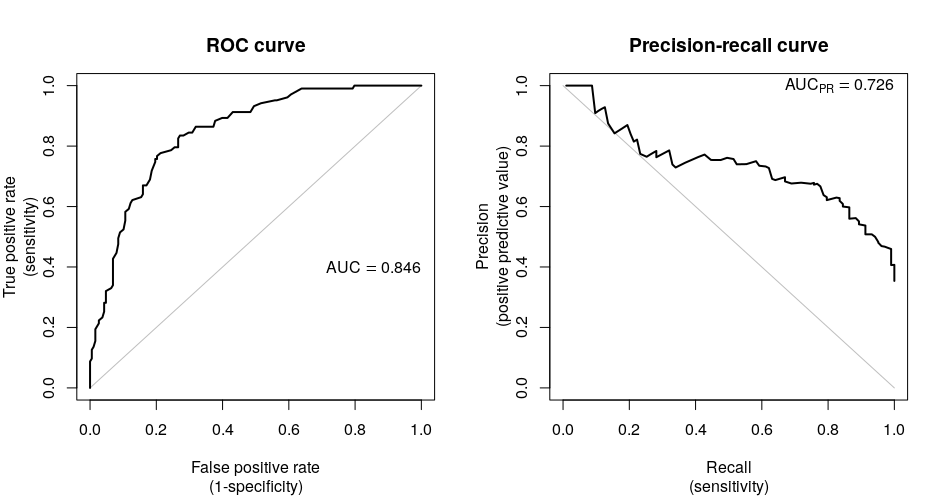
\includegraphics[width=\linewidth]{obrazky-figures/roc_pr-1.png}
\caption{Example plots of a ROC curve and a PR curve~\cite{barbosa_2020}.}
\label{fig:rog-pr-curves}
\end{figure}




\section{Other classification algorithms}
\label{other-classification-algorithms}
Before the introduction to artificial neural networks, this section briefly introduces a few other classification algorithms.


\subsection*{Logistic regression}
\label{logistic-regression}
Similar to how linear regression predicts continuous values by assuming a linear relationship
between dependent and independent variables (useful for regression tasks), logistic regression divides elements 
into two groups based on a set probability threshold (often called decision boundary),
which makes it a suitable technique for binary classification.

Instead of assuming that the data follow a linear function, they are modeled
using a sigmoid function (Figure~\ref{fig:sigmoid}).The range of this function, the interval between 0 and 1,
can then represent the probability of an instance belonging to a certain class.
This probability then rounds to either 0 or 1 depending on whether it lies above 
or below the set threshold.

\begin{figure}[!hb]
\centering
\begin{tikzpicture}
    \begin{axis}[
    xmin=-6, xmax=6,
    ymin=0, ymax=1,
    legend pos = north west,
    grid=both,
    ytick distance=0.25,
    height = 0.34\textwidth,
    width = 0.48\textwidth
    ]
        \addplot[domain=-6:6] {1/(1+exp(-x))};
        \addplot[red, dashed, domain=-6:6] {0.5};
        \legend{$\frac{1}{1 + e^{-x}}$, threshold}
    \end{axis}
\end{tikzpicture}
\caption{Graph of a sigmoid function and a threshold set to 0.5.}
\label{fig:sigmoid}
\end{figure}

%While training this type of classifier, we are basically trying to find the
%coefficients $\beta_{0}$ and $\beta_{1}$ for logistic function in the form:
%$p(x) = \frac{1}{1 + e^{-(\beta_{0} + \beta_{1}x)}}$.
%To punish incorrectly predicted values, logistic loss is used as the loss function~\ref{loss-function} for this method.
%Also, the threshold can be adjusted based on our needs, since in some cases,
%it may be favorable to minimize either the number of false positive or false negative predictions.


\subsection*{Naive Bayes classifiers}
\label{naive-bayes-classifiers}
Naive Bayes classifiers are a family of probabilistic machine learning algorithms based on the Bayes theorem 
\eqref{eq:bayes}.
They always assume that all the features of an instance being classified are independent of each other,
and their contribution to the final outcome is equal. These assumptions are generally not present in the real world,
hence the name ``Naive''.
\begin{equation}
\label{eq:bayes}
P(A|B) = \frac{P(B|A) \ P(A)}{P(B)}
\end{equation}

At first, the dataset is converted into frequency tables, counting the numbers of occurrences
of different feature values. From this table, a likehood table is generated by finding the propabilities
of given features. After that, the Bayes theorem is used to calculate the posterior probabilities
of the object belonging to a certain class based on its features.
There are three types of Naive Bayes classifiers---Multinomial, Benoulli and Gaussian.


\subsection*{Decision trees}
\label{decision-trees}
Decision trees model the classification or regression process in the form of a tree structure.
Trees used for classification,
with a single discrete class label, are called classification trees.
They consist of decision nodes with two or more branches split according to a certain feature value
and leaf nodes representing classes.
An example can be seen in Figure~\ref{fig:decision-tree}.

\begin{figure}[!h]
    \centering
    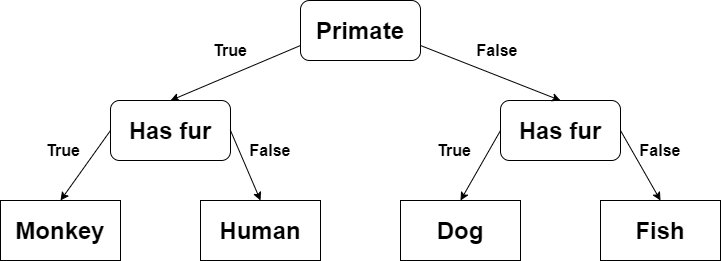
\includegraphics[scale=0.5]{obrazky-figures/decision_tree.png}
    \caption{A very simple classification tree.}
    \label{fig:decision-tree}
\end{figure}

A decision tree is built using the ID3 algorithm~\cite{quinlan1986induction},
which utilizes entropy and information gain.
Entropy is used to calculate the homogenity of a sample. The more equally divided a sample is,
the higher its entropy. The information gain depends on the decrease in entropy
after each splitting of the dataset on a feature. At each step,
the goal is to find the feature that returns the highest information gain.

Random forest is an algorithm made out of multiple randomly created decision trees,
where each tree-node works on a random subset of features and the final output
is combined from outputs of the individual trees.
As declared by Fran\c{c}ois Chollet in~\cite[p. 16]{Deep-learning-with-Python}, ``random forests are applicable to
a wide rage of problems---you could say that they're almost always
the second-best algorithm for any shallow machine learning tasks''.


\subsection*{$k$-nearest neighbors algorithm}
\label{k-nearest-neighbors-algorithm}
This algorithm classifies new cases based on a similarity measure to already labeled cases.
The new instance inherits the label most common among its $k$-nearest neighbors
measured by a distance function, where $ k \geq 1 $.
Larger $k$ value generally increases the precision by reducing the overall noise,
but the optimal value for most datasets was found to be between 3 and 10.
The number of dimensions of the space the labeled instances occupy
is equal to the number of input features.
Individual feature measures should also be normalized,
so that their contribution to the outcome is ideally the same.



\subsection*{Support vector machines}
\label{support-vector-machines}
A support vector machine (SVM) finds the hyperplane in an $N$-dimensional space
(where $N$ is the number of input features) separating the two classes
and maximizing the margin between them.
Support vectors are data points
that are closer to the hyperplane and influence its position and orientation.
For 2 input features, the classes are separated by a line,
for 3 of them, a the line is replaced by a plane and this goes on
into higher dimensions as the number of features increases.
For data that's not linearly separable,  one can use a non-linear SVM,
which utilizes Kernel functions that transform non-linear spaces into higher-dimensional linear spaces.



To classify a new sample, we take the output of a linear function.
If the output is greater than 1, the first class is predicted,
and if the output is smaller than -1, the other class is predicted.
The interval between -1 and 1 acts only as a margin, in contrast
to how logistic regression works. % MAYBE REF








\chapter{Artificial neural networks}
\label{artificial-neural-networks}
Artificial neural networks (ANNs), usually simply called neural networks (NNs),
are computational systems inspired by the function of biological neural networks.
They are at the heart of deep learning algorithms, a subset of machine learning algorithms.
Neural networks can be used for many kinds of tasks, including classification, pattern recognition or 
detection, clustering, and many others.
Some of the most notable real world applications include facial recognition, voice recognition,
weather forecasting, or studying the behavior of social media users.

This chapter serves as a gradual introduction to NNs, which begins by introducing
their basic building blocks in section~\ref{artificial-neuron},
moving up to their structure and behavior in section~\ref{artificial-neural-network}.
Section~\ref{training-a-neural-network} covers the principles of their training
and common problems to look out for while training them to solve classification problems.
The last section,~\ref{main-types-of-neural-networks}, explains
the differences between the main NN types and their use cases.




\section{Artificial neuron}
\label{artificial-neuron}
Artificial neurons~\cite[p. 5]{Suzuki_11} are the basic building blocks of every artificial neural network.
A biological neuron is made out of dendrites, which act as the input vector,
cell body (soma), which acts as the summation function, and axon, which gets its signal from the summation behavior
inside the soma and transmits the signal to other cells in the body including other neurons.
An artificial neuron (Figure~\ref{fig:artificial-neuron})
is a mathematical function basically mimicking a biological neuron.
It takes the sum of its one or more inputs, each individually multiplied by its assigned weight,
and then adds a constant value called bias to the sum. The sum is then passed through
a function known as an activation function (also called transfer function), which ``fires''
to pass the information to subsequent neurons.
\begin{figure}[!ht]
    \centering
    \begin{tikzpicture}[
    init/.style={
        draw,
        circle,
        inner sep=2pt,
        font=\Huge,
        join = by -latex
    },
    squa/.style={
        draw,
        inner sep=2pt,
        font=\Large,
        join = by -latex
    },
    start chain=2,node distance=17mm
    ]
    \node[on chain=2] 
        (x2) {$x_2$};
    \node[on chain=2,join=by o-latex] 
         {$w_2$};
    \node[on chain=2,init] (sigma) 
        {$\displaystyle\Sigma$};
    \node[on chain=2,squa,label=above:{\parbox{2cm}{\centering Activation \\ function}}]   
        {$f$};
    \node[on chain=2,label=above:Output,join=by -latex] 
        {$y$};
    \begin{scope}[start chain=1]
    \node[on chain=1] at (0,1.1cm) 
        (x1) {$x_1$};
    \node[on chain=1,label=above:Weights,join=by o-latex] 
        (w1) {$w_1$};
    \end{scope}
    \begin{scope}[start chain=3]
    \node[on chain=3] at (0,-1.1cm) 
        (x3) {$x_3$};
    \node[on chain=3,join=by o-latex] 
         (w3) {$w_3$};
    \end{scope}
    \node[label=above:\parbox{2cm}{\centering Bias \\ $b$}] at (sigma|-0,1.3cm) (b) {};
    \draw[-latex] (w1) -- (sigma);
    \draw[-latex] (w3) -- (sigma);
    \draw[o-latex] (b) -- (sigma);
    \draw[decorate,decoration={brace,mirror}] (x1.north west) -- node[left=10pt] {Inputs} (x3.south west);
    \end{tikzpicture}
    \caption{Example of an artificial neuron with three inputs.}
    \label{fig:artificial-neuron}
\end{figure}

The mechanism of an artificial neuron can be described mathematically:
\begin{equation}
\label{eq:neuron}
    y = f \bigg( b + \sum_{i=1}^n x_i w_i \bigg)
    =
    f \bigg( \sum_{i=0}^n x_i w_i \bigg)%, x_0 = 1 \wedge w_0 = b
\end{equation}
where $x_i$ is the $i$-th input of the neuron out of its $n$ total inputs,
$w_i$ is the weight assigned to the $i$-th input,
$b$ is bias, often represented by bias input $x_0 = 1$ with weight $w_0 = b$,
$f$ is an activation function and $y$ is the neuron's output.

The perceptron algorithm,
invented in 1958 at the Cornell Aeronautical Laboratory by Frank Rosenblatt~\cite{rosenblatt1958perceptron},
is considered to be the first artificial neural network, although it only consists of a single neuron with
a binary step activation function (see figure~\ref{fig:activation-functions}).


\subsection*{Activation function}
\label{activation-function}
Activation function is the part of a neuron that makes the final decision whether it should ``fire'' or not.
It can be as simple as a binary step (activates above certain threshold) function or a linear function,
but only when a non-linear function is used, then a two-layer neural network can be proven to be
a universal function approximator~\cite{cybenko1989approximation}. When multiple layers use
a linear activation function, the entire network is equivalent to a single-layer model,
since the output of each layer is a linear combination of the inputs, and hence, the overall output can be expressed as a single linear equation.

There are many different activation functions, each better suited for different scenarios.
Some of the most common ones include sigmoid---activation
function of choice for binary classification, already seen in Figure ~\ref{fig:sigmoid},
tanh (hyperbolic tangent), which usually finds applications
in recurrent neural networks (introduced later in section~\ref{main-types-of-neural-networks})
for natural language processing and speech recognition,
ReLU (Rectified Linear Unit),
which outperforms both sigmoid and tanh in computational speed,
and softmax, used to build multi-class classifiers.
Some of the mentioned activation functions are shown in Figure~\ref{fig:activation-functions}.

\begin{figure}[!ht]
\centering
\begin{tikzpicture}
    \begin{axis}[
    xmin=-2, xmax=1,
    ymin=-0.1, ymax=1.1,
    legend pos = north west,
    grid=both,
    ytick distance=0.5,
    xtick distance=1,
    height = 0.33\textwidth,
    width = 0.36\textwidth,
    legend style={cells={align=left}}
    ]
        \addplot[domain=-2:0] {0};
        \draw (0,0) -- (0,1);
        \addplot[domain=0:1] {1};
        \addlegendentry{0, $x<0$\\1, $x\geq0$}
    \end{axis}
\end{tikzpicture}
%
\begin{tikzpicture}
    \begin{axis}[
    xmin=-3, xmax=3,
    ymin=-1, ymax=1,
    legend pos = north west,
    grid=both,
    ytick distance=0.5,
    xtick distance=1,
    height = 0.33\textwidth,
    width = 0.36\textwidth
    ]
        \addplot[domain=-3:3] {tanh(x)};
        \legend{$\frac{e^x-e^{-x}}{e^x+e^{-x}}$}
    \end{axis}
\end{tikzpicture}
%
\begin{tikzpicture}
    \begin{axis}[
    xmin=-3, xmax=3,
    ymin=-0.3, ymax=3,
    legend pos = north west,
    grid=both,
    ytick distance=1,
    xtick distance=1,
    height = 0.33\textwidth,
    width = 0.36\textwidth
    ]
        \addplot[domain=-6:6] {max(0,x)};
        \addlegendentry{$max(0, x)$}
    \end{axis}
\end{tikzpicture}
\caption{Graphs of binary step (left), tanh (middle) and ReLU (right) activation functions.}
\label{fig:activation-functions}
\end{figure}




\section{Artificial neural network}
\label{artificial-neural-network}
A collection of interconnected artificial neurons can form an artificial neural network
\cite[p. 6]{Suzuki_11}.
An ANN is comprised of layers of neurons including the input layer, output layer,
and any number of layers between them, called hidden layers.
Neural networks can be visualised with graphs,
where each node represents a neuron and edges represent connections between them,
as shown in Figure~\ref{fig:deep-neural-network}.
The certain ways in which individual neurons
can be connected are called topologies.

At first, the input layer takes an input in the form of numerical data.
The hidden layers, present between input layer and output layer,
perform all the calculations to find hidden features and patterns in the data.
The input therefore goes through a series of transformations through succeeding layers,
which finally results in an output conveyed using the output layer.
In contrast with traditional computing models,
an NN acts as a black box, in the sense
that one cannot know what abstractly happens inside, since the network
learns by exposure to labeled data and ``stores the gained knowledge''
by tweaking its parameters (weights of the inputs of its neurons).
Knowledge in the form of many floating point numbers is obviously not very human-readable.


\subsection*{Topologies of neural networks}
\label{topologies-of-neural-networks}
The topology (also called architecture or structure)
of a neural network plays a fundamental role in its functionality and performance~\cite{fiesler1996topologies}.
When building an NN to solve a specific problem, there is no single topology best suited for it,
and while there are some empirically derived guidelines one can follow, it is mostly a matter of trial and error.
One thing to keep in mind is that while adding more layers allows an NN to learn more complex patterns,
it makes the network harder to train and much more prone to overfitting~\cite[p. 104]{Deep-learning-with-Python},
a very common problem explained later near the end of section~\ref{training-a-neural-network}.

One way to classify different NN topologies is distinguishing between
feed-forward neural networks (FFNNs) and recurrent neural networks (RNNs),
whose direct comparison is shown in figure~\ref{fig:feedforward-vs-recurrent}.
In a FFNN, the information flows in only one direction,
so any layer can only gain information from the previous layers.
In contrast, RNNs (often called feedback NNs) can have
signals traveling in both directions by introducing loops---edges
going from a given neuron to a neuron in either some previous layer or the current layer,
which can include the neuron itself. These feedback loops introduce the concept
of a network's memory, which is why these networks are used for processing
sequential data, where context matters a lot, such as recognizing spoken sequences,
detecting the next word/letter in a text, or even music
composition\footnote{Note that in the context of music composition, the term recurrent neural networks
refers to their use as generative models, where the network is trained to generate new music samples
based on a given input sequence}.
%\pagebreak

\begin{figure}[!h]
\def\layersep{3cm}
\def\outputlen{2cm}
\def\heightunit{cm*0.6}
\centering
% Feedforward network on the left
\begin{tikzpicture}[shorten >=1pt,->,draw=black, node distance=\layersep]
    \tikzstyle{every pin edge}=[<-,shorten <=1pt]
    \tikzstyle{input neuron}=[circle, minimum width=10pt, fill, inner sep=0pt];
    \tikzstyle{hidden neuron}=[circle, minimum width=30pt, draw, inner sep=0pt];
    \tikzstyle{invisible neuron}=[draw=none]
    
    % Draw the input layer nodes
    \foreach \name / \y in {1,3,5,7}
        \node[input neuron] (I-\name) at (0,-\y \heightunit) {};
        
    % Draw the hidden layer nodes
    \foreach \name / \y in {1,4,7}
        \path[yshift=0.0cm]
            node[hidden neuron] (H-\name) at (\layersep,-\y \heightunit) {};
            
    % Connect every node in the input layer with every node in the hidden layer
    \foreach \source in {1,3,5,7}
        \foreach \dest in {1,4,7}
            \path (I-\source) edge (H-\dest);
            
    % Draw invisible neurons
    \foreach \name / \y in {1,4,7}
        \path[yshift=0.0cm]
            node[invisible neuron] (O-\name) at (\layersep+\outputlen,-\y \heightunit) {};
            
    % Connect every node in the hidden layer with every node in the invisible layer
    \foreach \num in {1,4,7}
            \path (H-\num) edge (O-\num);
            
\end{tikzpicture}
\qquad\qquad%
% Recurrent network on the right
\begin{tikzpicture}[shorten >=1pt,->,draw=black, node distance=\layersep]
    \tikzstyle{every pin edge}=[<-,shorten <=1pt]
    \tikzstyle{input neuron}=[circle, minimum width=10pt, fill, inner sep=0pt];
    \tikzstyle{hidden neuron}=[circle, minimum width=30pt, draw, inner sep=0pt];
    \tikzstyle{invisible neuron}=[draw=none]
    
    % Draw the input layer nodes
    \foreach \name / \y in {1,3,5,7}
        \node[input neuron] (I-\name) at (0,-\y \heightunit) {};
        
    % Draw the hidden layer nodes
    \foreach \name / \y in {1,4,7}
        \path[yshift=0.0cm]
            node[hidden neuron] (H-\name) at (\layersep,-\y \heightunit) {};
            
    % Connect every node in the input layer with every node in the hidden layer
    \foreach \source in {1,3,5,7}
        \foreach \dest in {1,4,7}
            \path (I-\source) edge (H-\dest);
            
    % Draw invisible neurons
    \foreach \name / \y in {1,4,7}
        \path[yshift=0.0cm]
            node[invisible neuron] (O-\name) at (\layersep+\outputlen,-\y \heightunit) {};
            
    % Connect every node in the hidden layer with every node in the invisible layer
    \foreach \num in {1,4,7}
            \path (H-\num) edge (O-\num);
            
    % Draw curved lines for the nodes in hidden layer
    \draw[thick,->,shorten >=1pt] (H-1) to [out=-30,in=30,loop,looseness=1] (H-4);
    \draw[thick,->,shorten >=1pt] (H-4) to [out=100,in=-100,loop,looseness=1] (H-1);
    \draw[thick,->,shorten >=1pt] (H-4) to [out=-30,in=30,loop,looseness=1] (H-7);
    \draw[thick,->,shorten >=1pt] (H-7) to [out=100,in=-100,loop,looseness=1] (H-4);
    
\end{tikzpicture}
\caption{The comparison between feed-forward (left) and recurrent (right) neural networks.
While FFNNs allow the signal to travel one way only, RNNs contain feedback loops.}
\label{fig:feedforward-vs-recurrent}
\end{figure}

With the advancement in digital technologies in the recent years,
the demand for analyzing complex, high dimensional, and noise-contaminated
datasets has risen quite a lot. This led to a rapid development of deep learning,
part of a broader family of machine learning methods utilizing NNs.
The adjective ``deep'' refers to the use of multiple layers in the network,
which is then referred to as a deep neural network (DNN).
While not being a formally defined rule, an ANN should contain at least
two hidden layers to be called a DNN.
The complexity of these networks makes them a very powerful tool
for solving real-life problems.
An example of a DNN is visualized in figure~\ref{fig:deep-neural-network}.


\begin{figure}[!ht]
\centering
\begin{tikzpicture}[x=2.3cm,y=1.0cm]
  \message{^^JNeural network large}
  \readlist\Nnod{6,7,7,7,7,7,4} % array of number of nodes per layer
  
  \message{^^J  Layer}
  \foreachitem \N \in \Nnod{ % loop over layers
    \def\lay{\Ncnt} % alias of index of current layer
    \pgfmathsetmacro\prev{int(\Ncnt-1)} % number of previous layer
    \message{\lay,}
    \foreach \i [evaluate={\y=\N/2-\i; \x=\lay; \n=\nstyle;
                           \nprev=int(\prev<\Nnodlen?min(2,\prev):3);}] in {1,...,\N}{ % loop over nodes
      
      % NODES
      %\node[node \n,outer sep=0.6,minimum size=18] (N\lay-\i) at (\x,\y) {};
      \coordinate (N\lay-\i) at (\x,\y);
      
      % CONNECTIONS
      \ifnum\lay>1 % connect to previous layer
        \foreach \j in {1,...,\Nnod[\prev]}{ % loop over nodes in previous layer
          \draw[connect,white,line width=1.2] (N\prev-\j) -- (N\lay-\i);
          \draw[connect] (N\prev-\j) -- (N\lay-\i);
          %\draw[connect] (N\prev-\j.0) -- (N\lay-\i.180); % connect to left
          \node[node \nprev,minimum size=18] at (N\prev-\j) {}; % draw node over lines
        }
        \ifnum \lay=\Nnodlen % draw last node over lines
          \node[node \n,minimum size=18] at (N\lay-\i) {};
        \fi
      \fi % else: nothing to connect first layer
      
    }
  }
  % LABELS
  \node[above=0.5,align=center,mygreen!60!black] at (N1-1.90) {input\\layer};
  \node[above=0.5,align=center,myblue!60!black] at (N4-1.90) {hidden layers};
  \node[above=0.5,align=center,myred!60!black] at (N7-1.90) {output\\layer};
\end{tikzpicture}
\caption{A dense deep neural network. The original source code for generating
        this figure using TikZ\protect\footnotemark was taken from~\cite{neutelings_2022}.}
\label{fig:deep-neural-network}
\end{figure}
\footnotetext{\url{https://www.ctan.org/pkg/pgf}}


\subsection*{Tensor operations}
\label{tensor-operations}
``Much as any computer program can be ultimately reduced to a small set of binary
operations on binary inputs (AND, OR, NOT, and so on), all transformations learned
by artificial neural networks can be reduced to a handful of tensor operations applied
to tensors of numeric data''~\cite[p. 38]{Deep-learning-with-Python}. Tensors
are the basic data structure used not only by NNs,
but by all current machine learning systems.

Most students and researchers are probably familiar with scalars, vectors and matrices.
Those three structures can be referred to as 0D, 1D and 2D tensors (in this order),
since tensors are a generalization of matrices to an arbitrary number of dimensions,
as demonstrated in figure~\ref{fig:tensor-ranks}.
In the context of tensors, a dimension is often called an axis or the tensor's rank.
The key attributes of a tensor are its number of axes,
its shape (dimensions along each individual axis), and
in the context of programming---the data type of its contained data.
Even complex data can be broken down into a tensor---a dataset
consisting of multiple videos
can be represented as a 5D tensor, whose axes represent
a sample's order, number of the frame, x-coordinate (width),
y-coordinate (height), and (color) channels.
\pagebreak

\begin{figure}[!ht]
    \centering
    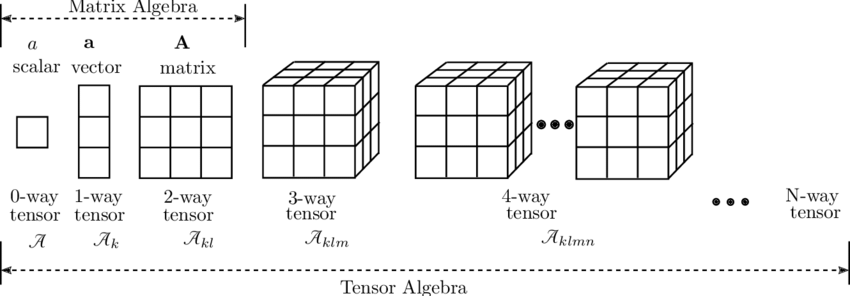
\includegraphics[width=\linewidth]{obrazky-figures/tensor-ranks.png}
    \caption{Tensors as generalizations of scalars, vectors and matrices~\cite{shulga2019tensor}.}
    \label{fig:tensor-ranks}
\end{figure}

Tensors can be added, multiplied and so on.
Each layer of an NN can be thought of as a function that
takes a tensor of a certain rank as its input, and returns a tensor of a certain rank as its output.
Since all tensor operations can also be interpreted geometrically,
the goal of a classification algorithm is basically just finding a chain of tensor
operations that ``uncrumbles'' the feature space in a way that separates the classes.




\section{Training a neural network}
\label{training-a-neural-network}
Training a neural network is the optimization process of finding the appropriate weights of its connections,
so that the difference between the network's output and the expected output is minimal.
This is possible thanks to a feedback loop algorithm
called backpropagation (short for backward propagation of errors),
which is the essence of NN training.

Though it is quite useful to know the basics of the mathematical foundation behind the training
mechanism (explained right in the following subsection),
a programmer doesn't have to worry too much about it when using a high level
deep learning API such as Keras~\cite{keras-documentation}.
From the practical standpoint, it's more important to know how to
preprocess data, split a dataset for training, validation and testing,
build a model with reasonable architecture comprised of layers
with activation functions fitting the given type of task, etc.
Some guidelines for these problems are spread throughout
this chapter, and mainly through the next chapter~\ref{the-keras-library},
which explores some of the extensive options Keras has to offer.


\subsection*{Loss function}
\label{loss-function}
Before diving into the training process itself, let's introduce a way
of measuring the difference between the expected output and the model's prediction.
This is the role of a loss function (synonymous with cost function or error function,
but cost sometimes refers to the average loss over the entire
training dataset).
It maps an event or values of one or more variables onto a real number representing
some ``cost'' associated with the event called loss, which we aim to minimize.

The most common loss for classification is cross-entropy,
which measures the performance of a classification model whose output is a probability value between 0 and 1.
Binary cross-entropy~\eqref{eq:binary-crossentropy}, a special case of cross-entropy with only two classes,
is not only the most commonly used loss for binary classification,
but is also often used for multi-label classification.
Assume that $y_i \in \{0,1\}$ marks the correct class of the $i$-th training sample and
$p_i$ is the predicted probability of the sample belonging to class 1.
\begin{equation}
\label{eq:binary-crossentropy}
    L_{BCE}(p_i, y_i) = -{(y_i\log(p_i) + (1 - y_i)\log(1 - p_i))}
\end{equation}
The general version of cross-entropy, used for multi-class classification, is often called categorical
cross-entropy~\eqref{eq:categorical-crossentropy}. Assume that $M$ is the total number of classes,
$\vec{\boldsymbol{y}_i}$ is a vector of size $M$ that indicates to which class the sample belongs,
$\vec{\boldsymbol{p}_i}$ is a vector of predicted probabilities for each class,
$y_{i,c}$ is a binary indicator whether sample $i$ belongs to class $c$
and $p_{i,c}$ is the corresponding predicted probability.
\begin{equation}
\label{eq:categorical-crossentropy}
    L_{CCE}(\vec{\boldsymbol{p}_i}, \vec{\boldsymbol{y}_i}) = -\sum_{c=1}^My_{i,c}\log(p_{i,c})
\end{equation}

Other classification losses include hinge loss~\eqref{eq:hinge-loss}, developed primarily for SVM model evaluation,
which apart from wrong predictions also penalizes right predictions that are not confident,
negative loglikelihood loss, and KL/JS divergence.
Note that in the case of hinge loss (in the version for binary classfication shown bellow),
$y_i \in \{-1,1\}$ and $p_i \in (-1,1)$.
\begin{equation}
\label{eq:hinge-loss}
    L_H(p_i, y_i) = max(0, 1 - y_i p_i)
\end{equation}


\subsection*{Gradient descent}
\label{gradient-descent}
The gradient of a function of $n$ variables can be interpreted as a vector pointing
in the direction of the fastest growth of the function. In the case of an NN, $n$ is equal
to the total number of weights in the network. Adjusting the network's weights
is done according to the gradient descend method, since we always want to minimize the loss function
with the goal of finding its global minimum.

Let's demonstrate this on a simple example of training a linear model consisting of a single
neuron without an activation function~\cite{sahu-power-of-single-neuron}. Training on each sample
can be thought of as finding solutions for linear equation~\eqref{eq:single-neuron-1}
with variables $a_0, a_1, ..., a_n$.
\begin{equation}
\label{eq:single-neuron-1}
    y = a_0 x_0 + a_1 x_1 + \dots + a_n x_n
\end{equation}
The model's guess based on its current weights can then be written down as equation~\eqref{eq:single-neuron-2}.
\begin{equation}
\label{eq:single-neuron-2}
    \hat{y} = w_0 x_0 + w_1 x_1 + \dots + w_n x_n
\end{equation}
We calculate the cost~\eqref{eq:single-neuron-3}
between the expected result and the model's prediction.
For the sake of the example, let's use the squared
error\footnote{Mean squared error (MSE) is the most commonly used loss function for regression.}
function, because it's easy to differentiate.
\begin{equation}
\label{eq:single-neuron-3}
    C = \frac{1}{2} (y - \hat{y})^2 = \frac{1}{2} (y - w_0 x_0 - w_1 x_1 - \dots - w_n x_n)^2
\end{equation}
We calculate the gradient of the cost~\eqref{eq:single-neuron-4},
which is nothing more than a vector consisting of its partial derivatives
each with respect to an individual weight~\eqref{eq:single-neuron-5}.
\begin{equation}
\label{eq:single-neuron-4}
    \nabla C(\vec{\boldsymbol{w}}) = \left\langle \frac{\partial C}{\partial w_0}, \frac{\partial C}{\partial w_1},
    \dots, \frac{\partial C}{\partial w_n} \right\rangle
\end{equation}
\begin{equation}
\label{eq:single-neuron-5}
    \frac{\partial C}{\partial w_i} = \frac{1}{2} \cdot 2 (y - w_0 x_0 - w_1 x_1 - \dots - w_n x_n) (-x_i)
\end{equation}
Moving to the final step~\eqref{eq:single-neuron-6},
the weights are updated by subtracting the calculated gradient multiplied by
the learning rate (denoted by $\eta$), a tuning parameter that determines the step size at
each iteration. While the learning rate can be as simple as a constant, there are
many optimization algorithms that scale it dynamically to
ensure faster and more reliable convergence towards the function's global minimum~\cite{ruder2016overview}.
\begin{equation}
\label{eq:single-neuron-6}
    \vec{\boldsymbol{w}} \leftarrow \vec{\boldsymbol{w}} - \eta \cdot \nabla C(\vec{\boldsymbol{w}})
    \Longleftrightarrow
    \forall i \in \{0,1,...,n\}:
    w_i \leftarrow w_i - \eta \cdot \frac{\partial C}{\partial w_i}
\end{equation}
These steps should be repeated until the algorithm converges.
This special case of calculating the cost for every iteration is called stochastic gradient descent.
In practice, the cost is usually calculated as the average loss over batches of training samples and sometimes even over entire epochs\footnote{An epoch is a single iteration over the entire training dataset.}.


\subsection*{Backpropagation}
\label{backpropagation}
Backpropagation, proposed back in 1986 by David E. Rumelhart~\cite{rumelhart1986learning},
is an efficient method of computing gradients in directed graphs of computations,
such as multi-layer neural networks.
When training an NN, every iteration consists of two passes---the forward pass and
the backward pass. In the forward pass, the data is fed to the input layer, goes through
the hidden layers and finally at the output layer, the network's prediction gets produced,
based on which the network's error can be calculated via the loss function.
In the backward pass, the flow is reversed so that the error gets propagated from the output
layer all the way back to the input layer, while updating the weights in each layer.
This process of propagating the error backwards is called backward propagation, or simply backpropagation.

The following interpretation of the backpropagation algorithm~\ref{alg:backpropagation}
draws inspiration from~\cite{FITMT16598} and~\cite{FITBT21764}.
To understand the notation, $x_{ij}^{(l)}$ is the $i$-th input of neuron $j$ in layer $l$
and $w_{ij}^{(l)}$ is the associated weight.
The weighted sum computed by neuron $j$ in layer $l$ is denoted by $z_j^{(l)}$, which then transforms to
the neuron's output $y_j^{(l)}$ by passing through its activation function $f$.
Since this time the neurons have an activation function, as wasn't the case in the example in previous subsection,
it was appropriate to break down the expressions inside step 4 using the chain rule,
which states that $f((g(x))' = f'(g(x)) g'(x)$.

\begin{algorithm}[H]
\caption{Backpropagation}
\label{alg:backpropagation}
\begin{enumerate}
    \setlength{\parsep}{5pt}
    \item \textbf{Initialization}
    
    Set all weights within the network to some small initial value.
    
    $ w_{ij}^{(l)}(0) = $ \textit{some small initial value}
    
    Set the iteration counter to 0.
    
    $ p = 0 $
    
    \item \textbf{Forward pass}
    
    Calculate the output of every neuron $j$ in each layer $l$ starting from the first hidden layer
    and ending with the output layer (the input layer only passes raw input).
    
     $y_j^{(l)}(p) = f \left( z_j^{(l)}(p) \right)
     = f\left( \displaystyle{\sum_{i=0}^n} \: w_{ij}^{(l)}(p) x_{ij}^{(l)}(p)  \right)$
     
     Note that $n$ is the number of inputs of neuron $j$ and $w_{0j} x_0$
     is its bias term.
     
     \item \textbf{Error calculation}
     
     Calculate the error $C(p)$ between the expected output for the current sample
     and the output obtained from the neuron(s) in the output layer.
     
     If the training data is split into batches, repeat step 2 for every sample
     in the current batch and then calculate $C(p)$ as the average loss across the batch.
    
     \item \textbf{Backward pass} % or weights adjustment
     
     First, calculate the derivatives of the error in terms of the weights
     between the last hidden layer and the output layer.
     
     $ \cfrac{\partial C}{\partial w_{ij}^{(out)}} = \cfrac{\partial C}{\partial y_j^{(out)}}
       \cfrac{\partial y_j^{(out)}}{\partial z_j^{(out)}}
       \cfrac{\partial z_j^{(out)}}{\partial w_{ij}^{(out)}} $
       
     Continue calculating derivatives of the error in terms of the weights between all the remaining
     pairs of neighboring layers going from right to left.
       
     $ \cfrac{\partial C}{\partial w_{ij}^{(l)}} = \cfrac{\partial C}{\partial y_j^{(l)}}
       \cfrac{\partial y_j^{(l)}}{\partial z_j^{(l)}}
       \cfrac{\partial z_j^{(l)}}{\partial w_{ij}^{(l)}} =
       \displaystyle{\sum_{k \in K}} \left( \cfrac{\partial C}{\partial y_k^{(l+1)}}
       \cfrac{\partial y_k^{(l+1)}}{\partial z_k^{(l+1)}}
       \cfrac{\partial z_k^{(l+1)}}{\partial y_j^{(l)}} \right)
       \cfrac{\partial y_j^{(l)}}{\partial z_j^{(l)}}
       \cfrac{\partial z_j^{(l)}}{\partial w_{ij}^{(l)}} $
       
    Note that $K$ is the set of all neurons in layer $l+1$ connected to neuron $j$.
    
    Update all weights within the network.
     
     $ w_{ij}^{(l)}(p+1) = w_{ij}^{(l)}(p) - \eta \cdot \cfrac{\partial C}{\partial w_{ij}^{(l)}} $
     
     \item \textbf{Repetition}
     
     Increase the iteration counter.
     
     $ p \leftarrow p + 1 $
     
     Continue with step 2, until the target number of iterations is reached or
     until the error decreases below a certain threshold.
     
\end{enumerate}
\end{algorithm}


\subsection*{Common problems}
\label{common-problems}
Training a neural network is not so straightforward, since there many pitfalls
one can find himself in.
Some problems can be caused by inappropriately chosen learning rate---a value too small
slows down the progress, while a value too high introduces oscillations and instabilities
leading to divergence. It is also not uncommon to get stuck
in a local minimum while performing gradient descent (since hardly any loss function
is convex), in which case it is recommended to introduce some element of randomness.

On a larger scale, the most common problem is probably overfitting~\cite[p. 104]{Deep-learning-with-Python}.
An NN is trained on a dataset which is meant to represent the problem it is being trained to solve,
but since the dataset contains only finite number of samples, it can only represent
a subset of the problem space. Overfitting occurs when the model becomes too accustomed
to its training data. It fails to generalize the problem and performs poorly when presented with new data.
It is caused by the model memorizing patterns in irrelevant information (noise) within the dataset,
which usually happens when the model trains for too long on sample data or when the model is too complex.
Some techniques to prevent overfitting (other than getting more training data)
include reducing the network's capacity by removing some hidden layers
or reducing the number of neurons in them, and applying regularization, which adds additional cost to the loss
function for larger weights. Three most popular regularization techniques are L1 and L2
regularization\footnote{Penalizing the total loss by either absolute values (L1) or squares (L2)
of the weights.}, and also introducing dropout layers,
which randomly remove certain features by randomly setting some inputs of a layer to zero.

The opposite phenomenon to overfitting is underfitting~\cite[p. 104]{Deep-learning-with-Python},
which occurs when the model is unable to accurately capture the relationship between input and output variables,
leading to high error rates on both the training set and unseen data.
This usually happens when there is simply not enough training data or the model is too simple.
Techniques to reduce underfitting include increasing the model's complexity, increasing the number of
features by performing feature engineering, removing unwanted noise from the data or simply
increasing the duration of the training.
Underfitting is usually easier to identify than overfitting,
since an overfitted model reaches high accuracy in training.
A visual interpretation of both underfitting and overfitting can be seen % or is shown
in figure~\ref{fig:underfitting-overfitting}.

\begin{figure}[!ht]
    \centering
    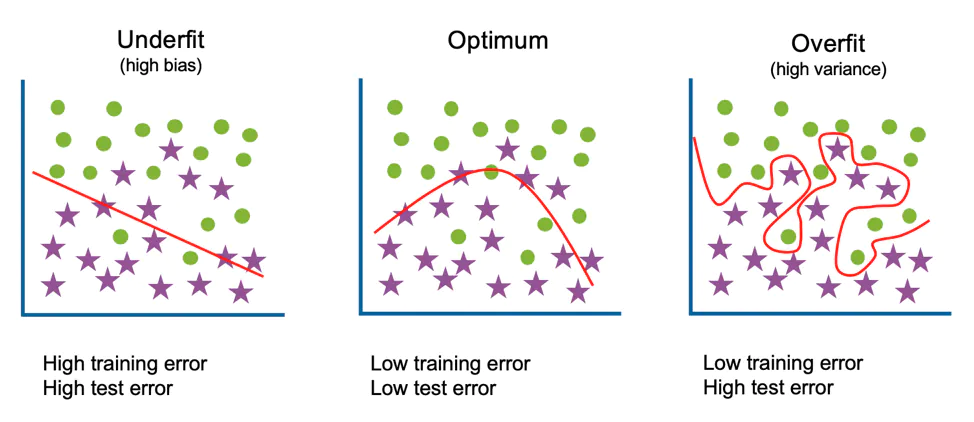
\includegraphics[width=\linewidth]{obrazky-figures/underfitting_overfitting.png}
    \caption{Visual interpretation of underfitting and overfitting~\cite{IBM-overfitting}.}
    \label{fig:underfitting-overfitting}
\end{figure}




\section{Main types of neural networks}
\label{main-types-of-neural-networks}
This section explains the differences between the three main ANN types.


\subsection*{Multi-layer perceptron}
\label{multi-layer-perceptron}
Multi-layer perceptron (MLP) refers to a standard feedforward neural network whose three or more layers are fully
connected~\footnote{A layer that is fully connected with its preceding layer is called a dense layer.}
and (except for the input layer) utilize some non-linear activation function.
A topology of an MLP may look like the one previously shown in figure~\ref{fig:deep-neural-network}.
Note that the ``perceptrons'' of which MLPs are composed of are not perceptrons in the strictest possible sense,
but rather ordinary artificial neurons,
since they can employ arbitrary activation functions (not limited to threshold-based functions).

Since an MLP accepts a vector (1D tensor) of numerical features as input, data is mostly
provided in a tabular format, such as csv~\footnote{A CSV (comma-separated values) file is a text file that has a
specific format which allows data to be saved in a table structured format.}
files or spreadsheets.
In these datasets, rows separate individual instances, while columns
separate individual features, including the class label in the case of classification problems.
MLPs can also work with more complicated data, such as images, text data, or timeseries data,
if there is a sensible way to convert the data into a vector. For instance, a 28x28 pixel grayscale image can be converted
to a vector consisting of 784 numerical features representing individual pixels.
The main problem with using MLPs for image classification is that they can only recognize global patterns.
For example, an MLP can be trained to classify different shapes if they're all similarly scaled and located in the same
part of an image, but fails to classify them once they're presented in different scales and locations.




\subsection*{Convolutional neural network}
\label{convolutional-neural-network}
A convolutional neural network (CNN/ConvNet) is an NN type most commonly used
for processing image data~\cite{cnn2015introduction},
since unlike an MLP, it has the ability to recognize local patterns in multidimensional data.
A CNN looks for spatial relations (relations between nearby pixels)
instead of only looking at an image as a whole---this property is called translation invariance
and allows the network to recognize objects regardless of their position in an image.
Capturing the spatial and temporal dependencies in an image is done through the
application of relevant filters.

The central part of any CNN, that also gave this NN type its name,
is the convolutional layer. Convolution is a mathematical operation, in this sense refering to
the process of adding each element of an image to its
local neighbors, weighted by a convolutional kernel, as shown in figure~\ref{fig:image-convolution}.
A convolutional layer contains a set of kernels, parameters of which are to be learned throughout the training.
Each kernel is used for detecting a specific feature in the data, creating a feature map.
A structure of multiple kernels stacked together is called a filter.
Two important terms when considering convolution are padding---a process
of adding layers of zeros around the image so that the kernel can overlap the image
in every possible position which has an element of the original image at the kernel's center,
so that the feature map keeps the size of the input image,
and stride---the number of elements traversed between steps.
A stride of more than 1 obviously downsamples the image even if it's padded along the edges.
\newpage

\begin{figure}[!ht]
\centering
\begin{tikzpicture}

	\matrix (mtr) [matrix of nodes,row sep=-\pgflinewidth, nodes={draw}]
	{
		0 & 1 & 1 & |[fill=red!30]| 1 & |[fill=red!30]| 0 & |[fill=red!30]| 0 & 0\\
		0 & 0 & 1 & |[fill=red!30]| 1 & |[fill=red!30]| 1 & |[fill=red!30]| 0 & 0\\
		0 & 0 & 0 & |[fill=red!30]| 1 & |[fill=red!30]| 1 & |[fill=red!30]| 1 & 0\\
		0 & 0 & 0 & 1 & 1 & 0 & 0\\
		0 & 0 & 1 & 1 & 0 & 0 & 0\\
		0 & 1 & 1 & 0 & 0 & 0 & 0\\
		1 & 1 & 0 & 0 & 0 & 0 & 0\\
	};

	\draw[very thick, red] (mtr-1-4.north west) rectangle (mtr-3-6.south east);

	\node [below= of mtr-5-4.south] (lm) {Input image};

	\node[right = 1em of mtr] (str) {$*$};

	\matrix (K) [right=1em of str,matrix of nodes,row sep=-\pgflinewidth, nodes={draw, fill=blue!30}]
	{
		1 & 0 & 1 \\
		0 & 1 & 0 \\
		1 & 0 & 1 \\
	};
	\node [below = of K-3-2.south, align=center, yshift=\baselineskip] (lk) {Convolution\\kernel};

	\node [right = 1em of K] (eq) {$=$};

	\matrix (ret) [right=1em of eq,matrix of nodes,row sep=-\pgflinewidth, nodes={draw}]
	{
		1 & 4 & 3 & |[fill=green!30]| 4 & 1\\
		1 & 2 & 4 & 3 & 3\\
		1 & 2 & 3 & 4 & 1\\
		1 & 3 & 3 & 1 & 1\\
		3 & 3 & 1 & 1 & 0\\
	};
	\node [below = of ret-4-3.south] (lim) {Feature map};

	\draw[very thick, green] (ret-1-4.north west) rectangle (ret-1-4.south east);

	\draw[densely dotted, blue, thick] (mtr-1-4.north west) -- (K-1-1.north west);
	\draw[densely dotted, blue, thick] (mtr-3-4.south west) -- (K-3-1.south west);
	\draw[densely dotted, blue, thick] (mtr-1-6.north east) -- (K-1-3.north east);
	\draw[densely dotted, blue, thick] (mtr-3-6.south east) -- (K-3-3.south east);

	\draw[densely dotted, green, thick] (ret-1-4.north west) -- (K-1-1.north west);
	\draw[densely dotted, green, thick] (ret-1-4.south west) -- (K-3-1.south west);
	\draw[densely dotted, green, thick] (ret-1-4.north east) -- (K-1-3.north east);
	\draw[densely dotted, green, thick] (ret-1-4.south east) -- (K-3-3.south east);

	\matrix (K) [right=1em of str,matrix of nodes,row sep=-\pgflinewidth, nodes={draw, fill=blue!10}]
	{
		1 & 0 & 1 \\
		0 & 1 & 0 \\
		1 & 0 & 1 \\
	};

	\draw[very thick, blue] (K-1-1.north west) rectangle (K-3-3.south east);

	\node[anchor=south east, inner sep=0.01em, blue] at (mtr-1-4.south east) (xx) {\scalebox{.5}{$\times 1$}};
	\node[anchor=south east, inner sep=0.01em, blue] at (mtr-1-5.south east) (xx) {\scalebox{.5}{$\times 0$}};
	\node[anchor=south east, inner sep=0.01em, blue] at (mtr-1-6.south east) (xx) {\scalebox{.5}{$\times 1$}};
	\node[anchor=south east, inner sep=0.01em, blue] at (mtr-2-4.south east) (xx) {\scalebox{.5}{$\times 0$}};
	\node[anchor=south east, inner sep=0.01em, blue] at (mtr-2-5.south east) (xx) {\scalebox{.5}{$\times 1$}};
	\node[anchor=south east, inner sep=0.01em, blue] at (mtr-2-6.south east) (xx) {\scalebox{.5}{$\times 0$}};
	\node[anchor=south east, inner sep=0.01em, blue] at (mtr-3-4.south east) (xx) {\scalebox{.5}{$\times 1$}};
	\node[anchor=south east, inner sep=0.01em, blue] at (mtr-3-5.south east) (xx) {\scalebox{.5}{$\times 0$}};
	\node[anchor=south east, inner sep=0.01em, blue] at (mtr-3-6.south east) (xx) {\scalebox{.5}{$\times 1$}};

\end{tikzpicture}
\caption{Convolution of a 7x7 image with a 3x3 kernel (no padding,
    stride set to 1)~\cite{tikzconvolution}.}
\label{fig:image-convolution}
\end{figure}

Although convolutional layers summarize the presence of features in an input image,
the feature maps they produce are sensitive to location of the features in the image.
A common approach for reaching local translation invariance is to downsample the feature map.
Although this can be easily achieved by changing the stride, a more robust and common
approach is to introduce pooling layers. Pooling transforms groups of elements (called patches) in a feature map
into single elements, based on the selected pooling operation---the most common ones are maximum pooling (max pooling),
which selects the highest value in the patch, and average pooling, which calculates the average of the
values. Both of these pooling operations are shown in figure~\ref{fig:pooling}.
Some non-linear function (e.g. ReLU) is usually applied to a feature map before it gets passed to
a pooling layer. It should also be noted that while pooling can help the network become more translation invariant,
it does not address its variance to other transformations such as rotations or changes in scale of an object,
and even though some special CNN architectures addressing this issue were already proposed~\cite{li2017rotation},
the usual way of combating this issue is to simply include slightly modified (rotated, mirrored, etc.)
copies of images already contained in the dataset when training---this is part of a technique
called data augmentation.

\begin{figure}[h!]
\centering
\begin{tikzpicture}
\matrix (mtra) [matrix of nodes, nodes={draw}]
{
    |[fill=red!15]| 3 & |[fill=red!15]| 5 & |[fill=blue!15]| 3 & |[fill=blue!15]| 8 \\
    |[fill=red!15]| 0 & |[fill=red!15]| 2 & |[fill=blue!15]| 1 & |[fill=blue!15]| 5 \\
    |[fill=green!15]| 0 & |[fill=green!15]| 9 & |[fill=orange!15]| 7 & |[fill=orange!15]| 2 \\
    |[fill=green!15]| 1 & |[fill=green!15]| 4 & |[fill=orange!15]| 2 & |[fill=orange!15]| 4 \\
};

\node[right = 1.5em of mtra] (opab) {$\longrightarrow$};

\node [below = 1.5em of opab, align=center, yshift=\baselineskip] (mp) {Max\\pooling};

\matrix (mtrb) [right=1.5em of opab, matrix of nodes, nodes={draw}]
{
    |[fill=red!15]| 5 & |[fill=blue!15]| 8 \\
    |[fill=green!15]| 9 & |[fill=orange!15]| 7 \\
};

\matrix (mtrc) [right=5em of mtrb, matrix of nodes, nodes={draw}]
{
    |[fill=red!15]| 3 & |[fill=red!15]| 5 & |[fill=blue!15]| 3 & |[fill=blue!15]| 8 \\
    |[fill=red!15]| 0 & |[fill=red!15]| 2 & |[fill=blue!15]| 1 & |[fill=blue!15]| 5 \\
    |[fill=green!15]| 0 & |[fill=green!15]| 9 & |[fill=orange!15]| 7 & |[fill=orange!15]| 2 \\
    |[fill=green!15]| 1 & |[fill=green!15]| 4 & |[fill=orange!15]| 2 & |[fill=orange!15]| 4 \\
};


\node[right = 1.5em of mtrc] (opcd) {$\longrightarrow$};

\node [below = 1.5em of opcd, align=center, yshift=\baselineskip] (mp) {Average\\pooling};

\matrix (mtrd) [right=1.5em of opcd, matrix of nodes, nodes={draw}]
{
    |[fill=red!15]| 2.5 & |[fill=blue!15]| 4.25 \\
    |[fill=green!15]| 3.5 & |[fill=orange!15]| 3.75 \\
};


\end{tikzpicture}
\caption{Application of 2x2 max pooling and 2x2 average pooling to a 4x4 feature map.}
\label{fig:pooling}
\end{figure}

The overall architecture of a CNN can be broken down into two parts, as can be seen in figure~\ref{fig:cnn-architecture}.
The first part, responsible for feature extraction, is made of convolutional layers,
each usually followed by a pooling layer. The first convolutional layer
is usually used to detect low-level features, such as horizontal or vertical lines, but the
deeper a convolutional layer is, the higher-level features it can recognize, such
as entire objects or even facial expressions.
The second part of a CNN, responsible for the classification itself, consists of dense layers
and essentially behaves as a standard MLP. Feature maps usually have more than one dimension,
but a dense layer only accepts a vector as input.
To solve this problem, we can introduce a flatten layer, which transforms all the final pooled
feature maps into a single large vector.

\begin{figure}[!ht]
    \centering
    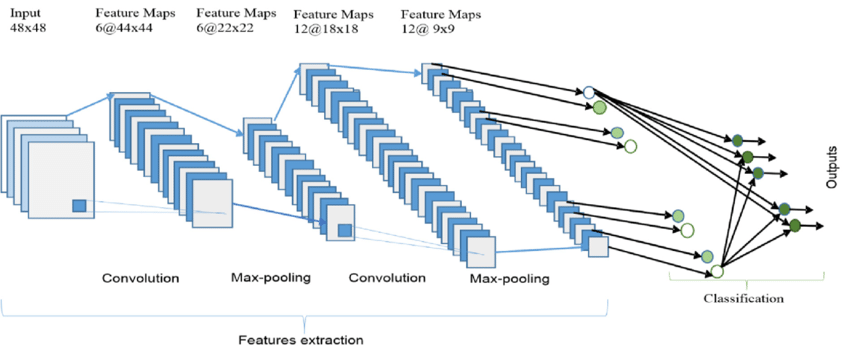
\includegraphics[width=\linewidth]{obrazky-figures/cnn-architecture.png}
    \caption{Architecture of a CNN composed of an input layer, multiple alternating
    convolution and max-pooling layers, one dense layer and an output
    layer~\cite[Figure~9]{soa-dl-theory-architectures}.}
    \label{fig:cnn-architecture}
\end{figure}


\subsection*{Recurrent neural network}
\label{recurrent-neural-network}
Sometimes we might want to work with sequential data (e.g. time series), where the chronological order
of elements creates a certain context.
Most prominent is natural language processing, which includes both text (as sequences
of either words or characters) and speech.
For this kind of problem,
let's consider a special NN type that has a sequential memory,
which provides the ability to remember preceding elements and take them into consideration.
This is called a recurrent neural network (RNN), and its concept is based
on David Rumelhart's work in 1986~\cite{rumelhart1986learning}.
Apart from sequence classification and regression, RNNs are also great for building generative models
that require a sequential output, such as generating text or even handwriting.

In an RNN, information gets passed not only to succeeding layers, but also backwards through
loops, as was previously shown in figure~\ref{fig:feedforward-vs-recurrent} when mentioning RNNs
in the context of NN topologies. Each recurrent cell has its
 hidden state, which is calculated as a function of
its previous hidden state and its input. This means that the network as a whole
has a hidden state, that strongly affects its response to a given input.

A huge problem RNNs face is their short-term memory caused by the vanishing gradient
problem~\cite{hochreiter1991untersuchungen},
from which they tend to suffer more than other NN architectures the more steps they process.
When a FFNN is trained using backpropagation, the backpropagated error signal typically decreases
exponentially as it propagates further from the output layer, making the weight adjustments
in those layers less prominent. All neurons that participated in the calculation
of the output get updated---this gets very complicated in the case of an RNN,
where it's not just the neurons preceeding the output layer, but all of the neurons
involved back in time, creating a long path for the error to propagate through.
This diminishes the effect of earlier inputs on the network's training.
To overcome this problem, two specialised versions of RNN were created.

Long Short Term Memory (LSTM), capable of remembering long sequences for a long period of time,
was introduced by Hochreiter and Schmidhuber in 1997~\cite{hochreiter1997long}.
The new hidden state of a LSTM cell is calculated not only from the previous hidden
state of the input, but also from information stored in the long term memory.
There is a total of three gates that LSTM uses---at each timestep, the input gate decides what information
will be stored in long term memory, the forget gate decides which of this information
will be kept or discarded, and the output gate calculates the new hidden state.

Gated recurrent unit (GRU), introduced in 2014 by Kyunghyun Cho~\cite{cho-gru},
is designed similarly as LSTM, but it aims to solve the same problem by incorporating
an operating mechanism that consists of the update gate, responsible for determining the amount
of previous information getting passed to the next state, and the reset gate,
which decides how much of the past information is going to be neglected (forgotten).
At first, it takes the input, and the previous hidden state multiplied by
the reset gate's output, which results in something called the candidate's hidden state.
This state, together with the update gate, is then used to calculate the current hidden state.
The cells of a standard RNN, LSTM and GRU are all shown in figure~\ref{fig:rnn-lstm-gru}.

\begin{figure}[!h]
    \centering
    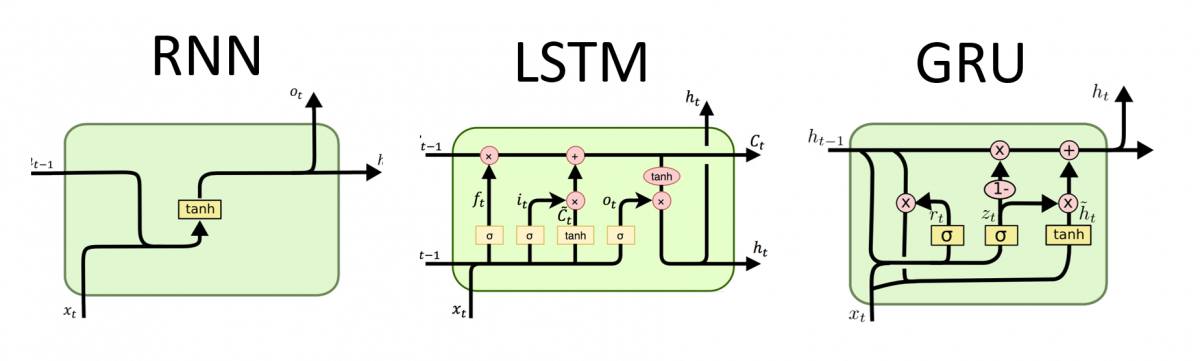
\includegraphics[width=\linewidth]{obrazky-figures/RNN-vs-LSTM-vs-GRU.png}
    \caption{Comparison of standard RNN cell, LSTM cell and GRU cell~\cite{rnn-lstm-gru}.}
    \label{fig:rnn-lstm-gru}
\end{figure}






\chapter{The Keras library}
\label{the-keras-library}
Keras is an open source library that provides a high-level interface for working with artificial
neural networks in Python\footnote{\url{https://www.python.org/}}.
It uses the TensorFlow\footnote{\url{https://www.tensorflow.org/}} library as its
backend\footnote{Up until version 2.3, Keras could also be configured to utilize a different library,
such as Theano or CNTK. Since version 2.4, only TensorFlow is supported. Keras has also been embedded
as part of the TensorFlow package since the release of TensorFlow 2.0.}, for which it provides
a high-level API that makes deep learning more accessible to a wider range of users through its ease of use.
Keras, written in Python, was developed with a focus on enabling fast experimentation,
with the core idea that ``being able to go from idea to result as fast as possible is key
to doing good research''~\cite{keras-documentation}.

Since the range of options Keras has to offer is very extensive,
the goal of this chapter is to explore some of its main offerings in the context of classification,
in the form of a guide starting with a model's building phase in section~\ref{building-a-model},
followed by it's compilation in section~\ref{compiling-a-model}, its training in section~\ref{training-a-model},
and finally its testing and general usage in final section~\ref{testing-and-using-a-model}.
Each section briefly introduces the many choices a user has along the way of solving a given
classification problem using Keras. Much of the information in this chapter is drawn from the official
Keras documentation~\cite{keras-documentation}, and from the book Deep Learning in
Python~\cite{Deep-learning-with-Python} written by Fran\c{c}ois Chollet, the author of Keras himself.




\section{Building a model}
\label{building-a-model}
There are three ways to create a model in Keras.
The most straightforward way is to use the \texttt{Sequential} class, which groups
a linear stack of layers into a sequential model with a single input and a single output.
The second option is using the Keras functional API, which is more flexible and capable of creating
models with non-linear topologies, shared layers, and even multiple inputs and outputs.
It provides an easy-to-use way of creating directed acyclic graphs of layers.
A direct comparison between using the \texttt{Sequential} class and using the functional API is shown
in listing~\ref{lst:sequential-vs-functional}.
The last option is to use model subclassing, by writing custom subclasses of the \texttt{Model} class
and the \texttt{Layer} class.

\begin{lstlisting}[caption={An MLP binary classification model built using the \texttt{Sequential} class
and an equivalent model built using the functional API.}, label={lst:sequential-vs-functional}]
import tensorflow as tf

model = tf.keras.Sequential()
model.add(tf.keras.layers.Dense(16, activation='relu', input_shape=(12,)))
model.add(tf.keras.layers.Dense(8, activation='relu'))
model.add(tf.keras.layers.Dense(1, activation='sigmoid'))

input_layer = tf.keras.Input(shape=(12,))
hidden_layer = tf.keras.layers.Dense(16, activation='relu')(input_layer)
hidden_layer = tf.keras.layers.Dense(8, activation='relu')(hidden_layer)
output_layer = tf.keras.layers.Dense(1, activation='sigmoid')(hidden_layer)
equivalent_model = tf.keras.Model(inputs=input_layer, outputs=output_layer)
\end{lstlisting}


\subsection*{Layers and activation functions}
\label{layers-and-activation-functions}
A model is series of layers grouped into a \texttt{Model} object with training and inference features.
Each layer consists of a tensor-in tensor-out computation function and usually also some state (the layer's weights).
The most basic is probably the \texttt{Dense} layer, which contains \texttt{units} number of neurons,
each connected to every neuron in the previous layer.
All the available layers can be grouped into the following categories:
\begin{itemize}
    \item \textbf{Core layers}: \texttt{Dense}, \texttt{Input} object, \texttt{Embedding}, \texttt{Activation},
    \texttt{Masking}, \texttt{Lambda}
    \item \textbf{Convolution layers}: \texttt{Conv1D}, \texttt{Conv2D}, \texttt{Conv3D}, \texttt{SeparableConv2D},\\ \texttt{DepthwiseConv2D}, \texttt{Conv2DTranspose}, etc.
    \item \textbf{Pooling layers}: \texttt{MaxPooling1D}, \texttt{AveragePooling2D}, \texttt{GlobalMaxPooling2D},\\
    \texttt{GlobalAveragePooling3D}, etc.
    \item \textbf{Recurrent layers}: \texttt{SimpleRNN}, \texttt{LSTM}, \texttt{GRU}, base \texttt{RNN},
    \texttt{ConvLSTM2D}, etc.
    \item \textbf{Other layer categories}: Preprocessing (e.g. \texttt{TextVectorization}),
    normalization (e.g. \texttt{BatchNormalization}), regularization (e.g. \texttt{Dropout}),
    attention, reshaping (e.g. \texttt{Reshape}, \texttt{Flatten}), merging, locally-connected layers,
    and activation layers
\end{itemize}

Every layer type accepts a different set of arguments, through which can the layer's behavior be modified.
These arguments range from obvious ones like the number of units or the activation function,
to very specific ones like the kernel regularizer function (which introduces weight decay).
Many of the arguments, including the activation function and the kernel regularizer,
can be passed either as an object instance, whose parameters can be tweaked,
or as a string identifier, in which case the default values will be used.
Both of these options are demonstrated in listing~\ref{lst:parameterized-layer}.

Activation function is without a doubt one of the most prominent layer attributes.
Keras \texttt{activations} module offers these built-in functions: \texttt{relu}, \texttt{sigmoid}, \texttt{softmax},
\texttt{softplus}, \texttt{softsign}, \texttt{tanh}, \texttt{selu}, \texttt{elu}
and \texttt{exponential}. Activation functions can not only be passed as an object instance or a string
identifier, but also added as a separate layer (see listing~\ref{lst:parameterized-layer}),
which is also the only was to use activations that maintain a state---for instance \texttt{PReLU},
and some other advanced activation functions such as \texttt{LeakyReLU}.

In a classification model, the hidden layers usually utilize either \texttt{relu},
\texttt{sigmoid} or \texttt{tanh} activation function. The output layer, however, depends on the given type
of classification. We use a \texttt{Dense} layer containing either a single neuron with \texttt{sigmoid}
for binary classification, \textit{number of classes} neurons with \texttt{softmax}
for multi-class classification as, shown at the end of listing~\ref{lst:parameterized-layer},
or \textit{number of classes} neurons with \texttt{sigmoid} for multi-label classification.

\begin{lstlisting}[caption={A CNN six-class classification model with
specifically parameterized layers.}, label={lst:parameterized-layer}]
model = tf.keras.Sequential()
model.add(tf.keras.layers.Conv2D(
    input_shape=(30, 30, 3), # 30x30 RGB image (3 color channels)
    filters=64, kernel_size=(3, 3), strides=(1, 1), padding='same',
    kernel_regularizer=tf.keras.regularizers.L2(0.001),
    kernel_initializer='zeros', bias_regularizer='l1',
    bias_initializer=tf.keras.initializers.Zeros()
))
model.add(tf.keras.layers.LeakyReLU(alpha=0.1))
... # Pooling, Flatten, Dense, etc.
model.add(tf.keras.layers.Dense(units=6, activation='softmax'))
\end{lstlisting}

Keras models can be saved to a file by the \texttt{save\_model()} function (or \texttt{Model}'s \texttt{save()} method)
and loaded by the \texttt{load\_model()} function. The same can be done with only the current weights instead
of the whole model, by the \texttt{Model}'s \texttt{save\_weights()} and \texttt{load\_weights()} methods.
The model's summary, which contains information about the consecutive layers (e.g. layer type, number of
trainable parameters), can be printed using \texttt{Model}'s \texttt{summary()} method.
Models can also be plotted and saved as an image using the \texttt{plot\_model()} function from Keras utilities.





\section{Compiling a model}
\label{compiling-a-model}
%first code snippet of compilation and saying you can pass as string (default params) or instance
%then 3 subsections about loss, optimizer, metrics
Once a model is built, the \texttt{Model}'s \texttt{compile()} method is used to configure
it for training. Apart from some very specific optional arguments,
we specify the optimizer and the loss function to be used for training, and a list of  metrics to be evaluated
during training and testing.
All of these can be again passed either as a object instance or as an string identifier (default parameters),
an example can be seen in listing~\ref{lst:compile}.

\begin{lstlisting}[caption={Configuring a Keras model for training using its \texttt{compile} method.},
                   label={lst:compile}]
model.compile(optimizer=tf.keras.optimizers.Adam(learning_rate=1e-3),
    loss=tf.keras.losses.BinaryCrossEntropy(),
    metrics=['accuracy', tf.keras.metrics.FalsePositives()])
\end{lstlisting}


\subsection*{Optimizer}
\label{optimizer}
An optimizer is an algorithm that dictates how the model's attributes, such as weights and learning rate,
are updated in response to the output of the loss function. The simplest optimizer Keras
offers is \texttt{SGD}, which is the stochastic gradient descent algorithm, with an optional
\texttt{momentum} hyperparameter that accelerates the descent in the relevant direction.

The other available optimizers tend to be more complicated, since they all belong to the family of adaptive
optimizers~\cite{ruder2016overview},
introduced to solve the issues of gradient descent. This includes \texttt{Adagrad},
which adapts the learning rate to perform more significant updates for rarely occurring features,
\texttt{Adadelta} and \texttt{RMSprop}, both of which improve the previous algorithm by taking a fixed number
of past gradients into consideration, and \texttt{Adam}---the overall most commonly
used optimizer, which adds to the advantages of all these previous algorithms by storing
an exponentially decaying average of past gradients (similar to momentum).
The remaining Keras optimizers are \texttt{Adamax}, \texttt{Nadam} and \texttt{Ftrl}.


\subsection*{Loss}
\label{loss}
As already explained in section~\ref{training-a-neural-network},
the purpose of a loss function is to compute the quantity that a model seeks to minimize during training.
The built-in losses Keras offers can be divided into three categories: Probabilistic losses, regression losses, and
hinge losses for ''maximum-margin'' classification. Since this thesis revolves around classification,
we can neglect regression losses, apart from maybe mentioning \texttt{MeanSquaredError} and
\texttt{MeanAbsoluteError} since these two are very common.

Cross-entropy based losses can be found in the probabilistic category.
For binary classification, we use \texttt{BinaryCrossentropy}, while for multi-class
classification, we can use either \texttt{CategoricalCrossentropy} in combination with
label-encoded (integer) class labels, or\\ \texttt{SparseCategoricalCrossentropy} with one-hot-encoded
class labels (both of these encoding techniques will be explained in the next section~\ref{training-a-model}).
The probabilistic losses also include \texttt{KLDivergence} (Kullback–Leibler divergence), which measures
a very similar quality to cross-entropy, and \texttt{Poisson}, used for regression with discrete variables.

The last category includes three versions of the hinge loss function: standard \texttt{Hinge},
\texttt{SquaredHinge} and \texttt{CategoricalHinge}. The usage of these losses in Keras is quite rare,
since they are mostly used for SVMs and only very rarely for NNs.


\subsection*{Metrics}
\label{metrics}
A metric is a function that is used to evaluate the performance of a model,
but unlike loss functions, the results from evaluating a metric are not used when training the model.
The built-in metrics can be grouped into six categories. Three of these
categories correspond to the three previously listed loss categories, since any loss function can also
be used as a metric. Also, there is only a single metric in the image segmentation category---\texttt{MeanIoU}
(mean Intersection over Union), used to measure the accuracy of an object detector.

Probably the most common are accuracy metrics, which tell us how often the model predicted the correct outcome.
When the metric \texttt{Accuracy} is specified,
Keras detects the output shape and automatically determines which type of accuracy shall be used
(but it can also be specified manually).
These include \texttt{BinaryAccuracy}, which calculates how often predictions match binary labels (binary classification),
\texttt{CategoricalAccuracy} and \texttt{SparseCategoricalAccuracy}, which calculate how often predictions match either one-hot labels or integer labels respectively (multi-class classification),
and finally\\ \texttt{TopKCategoricalAccuracy} and \texttt{SparseTopKCategoricalAccuracy}, which compute how often targets
are in the top \texttt{K} predictions (multi-class classification).

The last category contains classification metrics based on true/false positives and negatives,
implementing the metrics defined in section~\ref{evaluating-a-models-performance}.
The simplest of these metrics are naturally \texttt{TruePositives}, \texttt{TrueNegatives}, \texttt{FalsePositives} and
\texttt{FalseNegatives}, which are self-explanatory, while the most complex one is probably \texttt{AUC},
which approximates the AUC (Area under the curve) of the ROC or
PR curves. The remaining metrics are \texttt{Precision},
\texttt{Recall}, \texttt{PrecisionAtRecall}, which computes the best precision
where $recall \geq specified$ $value$, and \texttt{SensitivityAtSpecificity} complemented by \texttt{SpecificityAtSensitivity},
which compute the best sensitivity where $specificity \geq specified$ $value$ and vice versa.




\section{Training a model}
\label{training-a-model}
A Keras model can be trained either by calling its \texttt{fit()} method, which trains the model for a fixed number
of epochs, or the \texttt{train\_on\_batch()} method, which runs a single gradient update on a single batch of data.
The arguments of the \texttt{fit()} method include the input data (unlabeled samples), target data (corresponding
class labels), \texttt{batch\_size} (number of samples per gradient update), \texttt{epochs} (number of epochs to train
the model for), and some others. Keras is usually combined with other Python libraries, since the input and target data
passed to the \texttt{fit()} method can be in the form of Numpy\footnote{\url{https://numpy.org/}} arrays,
TensorFlow tensors, Pandas\footnote{\url{https://pandas.pydata.org/}} DataFrames, or some of the few other more
specialized formats, including a dictionary mapping input names to the corresponding array/tensors, suitable for
models that have named inputs.

Part of the training data can be used for the model's validation using either the \texttt{validation\_split}
or \texttt{validation\_data} argument of the \texttt{fit()} method. A validation dataset is a sample of data
held back from training the model, giving out an unbiased estimate of the model's performance,  which is especially
useful for monitoring the generalizability of the model and detecting overfitting.
The \texttt{fit()} method returns a \texttt{History} object, whose \texttt{History.history} attribute is a record of training loss
and metrics values at successive epochs, as well as validation loss and metrics values (if applicable).
Value of the \texttt{verbose} argument controls how much information will be printed at the end of each epoch,
such as the values of loss and metrics (also for validation if applicable), or even an animated progress bar.

Keras also offers a few built-in datasets provided by the \texttt{tf.keras.datasets} module.
These include famous datasets such as the MNIST\footnote{\url{http://yann.lecun.com/exdb/mnist/}}
handwritten digits classification dataset~\cite{deng2012mnist}, the IMDB movie review
sentiment classification
dataset\footnote{\url{https://ai.stanford.edu/~amaas/data/sentiment/}}~\cite{maas-EtAl:2011:ACL-HLT2011},
the CIFAR10 and CIFAR100 small images classification datasets\footnote{\url{http://www.cs.toronto.edu/~kriz/cifar.html}},
and three other datasets. Training a model on a built-in dataset using the \texttt{fit()} method is shown in listing~\ref{lst:model-fit}.

\begin{lstlisting}[caption={Training a Keras model on the built-in MNIST handwritten digits classification datasets using
the \texttt{Model}'s \texttt{fit()} method.}, label={lst:model-fit}]
# Loading the training and testing data
(X_train, y_train), (X_test, y_test) = tf.keras.datasets.mnist.load_data()
# Training the model
model.fit(X_train, y_train, batch_size=32, epochs=80, validation_split=0.1)
\end{lstlisting}


\subsection*{Data preprocessing}
\label{data-preprocessing-subsection}
Since a dataset is usually a set of measurements of some phenomena, the data often has to be transformed
into a form that an NN can accept as input. This includes encoding non-numerical categorical data into numerical
values and reshaping the input---for example, a 2D CNN usually expects an input of shape \texttt{(rows, cols, channels)}.
Reshaping can be done in advance (often using Numpy), or by including one or more \texttt{Reshape} layers in the model's
architecture. Even though Keras offers some utilities (e.g. the \texttt{to\_categorical} function),
external libraries including more advanced preprosessing tools, such as
scikit-learn\footnote{\url{https://scikit-learn.org}}, are usually used alongside Keras.

There are three main techniques for encoding categorical data. Label encoding (also called integer or ordinal
encoding) represents each of $n$ total categories as an integer (either from 1 to $n$ or 0 to $n-1$). Label encoding should
only be used in cases where there is some kind of hierarchical relationship between the categories. If we tried to encode,
let's say, a $color$ attribute in that way, the network would learn some unintended relationship based on the order in which
the colors were encoded, such as $red < green < yellow$. If no relationship is present between the categories, one-hot encoding
should be used, which means transforming each value into a vector of length $n$, with all of its components set to 0 except for the 
single one representing the given category, which is set to 1. The direct comparison of label and one-hot encoding on a weather 
feature example is shown in table~\ref{table:encoding}. The last technique is called learned embedding (or simply embedding)
and is based on mapping each category to a distinct vector, whose properties are adapted while training the NN, which allows
for miscellaneous relationships between the categories to be learned. This technique is often referred to as word embedding,
since it was originally developed to provide a distributed representation for words (e.g. allowing similar words to have
similar vector representations). 

\begin{table}[!ht]
\newcommand{\specialcell}[2][c]{%
  \begin{tabular}[#1]{@{}c@{}}#2\end{tabular}}
\centering
\begin{tabular}{|c|c|c|c|}
    \cline{1-4}
    \specialcell{\textbf{Sample}\\\textbf{number}} & \specialcell{\textbf{Default}\\\textbf{feature}} &
    \specialcell{\textbf{Label encoded}\\\textbf{feature}} & \specialcell{\textbf{One-hot encoded}\\\textbf{feature}} \\
    \cline{1-4}
    1 & \texttt{''sunny''} & 1 & [1, 0, 0] \\
    \cline{1-4}
    2 & \texttt{''cloudy''} & 2 & [0, 1, 0] \\
    \cline{1-4}
    3 & \texttt{''sunny''} & 1 & [1, 0, 0] \\ 
    \cline{1-4}
    4 & \texttt{''rainy''} & 3 & [0, 0, 1] \\
    \cline{1-4}
\end{tabular}
\caption{Direct comparison of label encoding and one-hot encoding.}
\label{table:encoding}
\end{table}

Further preprocessing can be done to optimize the training process, generally leading to better results~\cite{isik2012importance}. 
This includes techniques like data augmentation (explained in the CNN subsection of section~\ref{main-types-of-neural-networks}),
normalization, standardization and batch normalization. Normalization refers to scaling the values from different ranges to
a common range, usually the interval $(0, 1)$, while standardization refers to transforming the data such that the mean
of the data is equal to zero and the standard deviation to one. Batch normalization (\texttt{BatchNormalization} layer
in Keras) is based on normalising each batch individually, and is often used after convolutional layers.

% TRAIN TEST VALIDATION SPLIT
It is extremely important to use different data for training, validation and testing to check how well
the model is generalized and to detect overfitting in time.
While there is no optimal dataset split percentage, since it depends on the given problem,
three standard ways to split a dataset
(training|validation|testing) are 80\%|10\%|10\%, 70\%|15\%|15\% and 60\%|20\%|20\%. In general,
the larger a dataset is, the lesser proportion of the data is required for testing and validation.
However, much more important than finding good split percentages is to ensure that these three datasets are about
equally balanced with respect to the distinct classes and feature values.


\subsection*{Callbacks}
\label{callbacks}
In Keras, a callback is an object that can perform actions at various stages of training/testing
(before/after a batch,
at the start/end of an epoch, etc.). There are several built-in callbacks, such as \texttt{ModelCheckpoint},
which periodically saves the trained model (or its weights) to a file, \texttt{CSVLogger}, which streams
epoch results to a CSV file, or \texttt{EarlyStopping}, which stops the training when a monitored metric
had stopped improving.

To create a custom callback, we simply create a subclass of the \texttt{Callback} class and override a set of methods
called at various stages of training, testing and predicting, such as \texttt{on\_(train|test|predict)\_begin()},
\texttt{on\_(train|test|predict)\_batch\_end()}, \texttt{on\_epoch\_begin()}, etc.
A list of callbacks can be passed to the \texttt{fit()} method (and also to the \texttt{evaluate()} and \texttt{predict()}
methods introduced in the following section~\ref{testing-and-using-a-model}) via the \texttt{callbacks} argument,
as shown in listing~\ref{lst:callbacks}.

\begin{lstlisting}[caption={A class for a custom callback, and training a Keras model using its \texttt{fit()} method while
utilizing multiple callbacks, including the custom one.}, label={lst:callbacks}]
# Custom callback that prints a message after the training is finished
class CustomCallback(tf.keras.callbacks.Callback):
    def on_train_end(self, logs=None):
        print("Training is complete, have a nice day!")

my_callbacks = [tf.keras.EarlyStopping(patience=2), CustomCallback()]
model.fit(X_train, y_train, epochs=30, callbacks=my_callbacks)
\end{lstlisting}



\section{Testing and using a model}
\label{testing-and-using-a-model}
%para model evaluate a test on batch + code
The \texttt{Model}'s \texttt{evaluate()} method is used to test/evaluate a model's performance.
Its arguments include the testing data, the corresponding class labels, \texttt{batch\_size}, and a few
others, including \texttt{callbacks}. There are obviously no epochs, since each iteration would show the same
results. The \texttt{evaluate()} method, shown in listing~\ref{lst:evaluate}, returns the loss value and metrics
for the model in test mode (weights don't get updated), and also prints the relevant information
(controlled by the \texttt{verbose} argument).
Alternatively, the \texttt{test\_on\_batch()} method can be used instead, to test the model on a single batch of data.

\begin{lstlisting}[caption={Evaluating a model's accuracy on a testing dataset.}, label={lst:evaluate}]
scores = model.evaluate(X_test, y_test, return_dict=True)
# return_dict=True => metrics are stored in a dictionary instead of a list
print("Test accuracy: ", scores['accuracy'])
\end{lstlisting}

%para model predict and predict batch + code
The \texttt{Model}'s \texttt{predict()} method generates output predictions for given input samples,
as shown in listing~\ref{lst:predict}.
It accepts similar arguments to the \texttt{evaluate()} method, except for class labels,
since those are returned by the method as a Numpy array(s) of predictions.
For a small number of inputs that fit in one batch (marked as \texttt{X}), we can also use the \texttt{Model}'s
\texttt{\_\_call\_\_()} method as \texttt{predictions = model(X)}, or its \texttt{predict\_on\_batch()} method.

\begin{lstlisting}[caption={Using a model to predict class labels for a given set of data.}, label={lst:predict}]
predictions = model.predict(X)
# the predicted labels are stored in a list
for i in range(len(predictions)):
    print("Class prediction for ", i+1, ". sample:", predictions[i])
\end{lstlisting}

Apart from custom NN architectures created directly by the user, Keras also offers some pre-built deep learning models,
along with pre-trained weights, as Keras Applications, available from the \texttt{tensorflow.keras.applications} module.
They can be used for prediction, feature extraction, and fine-tuning\footnote{Finetuning means taking weights
of a trained neural network and using it as initialization for a new model being trained on data from the same domain.
It is primarily used to speed up the training process and overcome small dataset size.}.
These models include famous CNN architectures, such as three different versions of Inception
including Xception~\cite{DBLP:journals/corr/Chollet16a} (Extreme version of Inception),
used in the exemplary use case shown in listing~\ref{lst:xception},
multiple versions of ResNet~\cite{DBLP:journals/corr/HeZRS15}, many version of
EfficientNet~\cite{DBLP:journals/corr/abs-1905-11946}, and a few others.

\begin{lstlisting}[caption={Classifying an image of a hamster by using the Xception~\cite{DBLP:journals/corr/Chollet16a}
NN architecture along with weights
pre-trained on the ImageNet\protect\footnotemark dataset}, label={lst:xception}]
from tensorflow.keras.applications import xception
from tensorflow.keras.preprocessing.image import load_img, img_to_array
import numpy as np

# loading weights from training on the ImageNet dataset
model = xception.Xception(weights="imagenet", include_top=True)
# loading and preprocessing hamster image
img = load_img('hamster.png', target_size=(299,299))
img = img_to_array(img)
img = np.expand_dims(img, axis=0)
# making model predictions (top=3 => show 3 most probable classes)
x = xception.preprocess_input(img)
preds = model.predict(x)
print("Predicted: ", xception.decode_predictions(preds, top=3)[0])
# Predicted:  [('n02342885', 'hamster', 0.9340777),
# ('n03794056', 'mousetrap', 0.0025085167),
# ('n07714990', 'broccoli', 0.002150822)]
\end{lstlisting}
\footnotetext{\url{https://www.image-net.org}}








\chapter{Preparation of the experiments}
\label{preparation-of-the-experiments}
Now that NNs and Keras have been sufficiently introduced, it's time to move on to the practical part of the
thesis. The objective of the experiments is to choose 3 different datasets, each suited for a different type
of NNs (tabular for MLPs, image for CNNs, sequential for RNNs), create an NN(s) of each type for each of the
datasets, compare their performances, and experimentally find out how often can an NN, that's not intuitively suited
for a given task at first glance, outperform the one that is.

Since comparing NNs of different types is a bit like comparing apples to oranges, this chapter
focuses on preparation of the experiments in such a way, that the different NNs can actually
utilize their signature abilities sensibly to their advantage. This heavily depends on the choice of the datasets
in section~\ref{choosing-and-analyzing-the-datasets}, preprocessing of the data in section~\ref{data-preprocessing},
which dictates how the data will be interpreted by the individual types of NNs, and finally, the NNs' architectures
in section~\ref{choosing-the-neural-network-architectures}.




\section{Choosing and analyzing the datasets}
\label{choosing-and-analyzing-the-datasets}
%Zde popiš vyváženost tříd v datasetech formou  grafů, a různé další vlastnosti datasetů.
This section introduces the chosen datasets, along with the reasons for choosing them and some brief analysis of their compositions.


\subsection{Tabular data - MiniBooNE particle identification}
\label{dataset-tabular}
MiniBooNE (Booster Neutrino Experiment) is a Cherenkov detector experiment at
Fermilab\footnote{\url{https://www.fnal.gov/}} designed to observe neutrino 
oscillations. The MiniBooNE particle identification dataset had been obtained from the UCI Machine Learning
Repository~\cite{Dua:2019}
and contains records of 130,064 events (instances), each consisting of 50 individual particle measurements
(real numbers), and a
binary label that marks whether the instance was a signal event (1) or a background event (0). Since there are only
36,499 ($\approx 28$ \%) signal events, compared to the remaining 93,565 ($\approx 72$ \%) background events,
one might call this an imbalanced binary classification problem.

Due to the nature of the experiment the dataset captures, the features (particle measurements) in the scope of a 
single event are obviously not
really independent of each other, so the RNN and 1D--CNN might be able to make use of their unique abilities to
identify some hidden patterns the MLPs are unable to see. 


\subsection{Image data - Fashion-MNIST}
\label{dataset-image}
Fashion-MNIST~\cite{DBLP:journals/corr/abs-1708-07747} is a dataset consisting of 60,000 training
and 10,000 test grayscale images of clothes,
each belonging in one of the 10 distinct clothing categories shown in figure~\ref{fig:fashion-mnist-samples}.
It was developed as a modern drop-in replacement
for the original MNIST dataset, from which it had inherited the same image resolution (28x28), number of
target classes, and even the total number of samples and the distribution of target classes.
The data was extracted from
Zalando's\footnote{\url{https://github.com/zalandoresearch/fashion-mnist}}
arcticle images and the entire dataset is built into Keras in the exact same manner as the standard MNIST.

\begin{figure}[!ht]
    \centering
    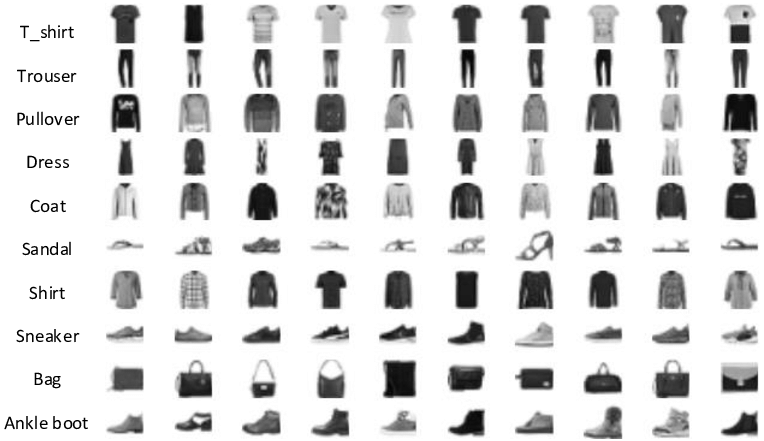
\includegraphics[width=\linewidth]{obrazky-figures/Fashion-MNIST_samples.png}
    \caption{Sample images from the Fahion-MNIST dataset~\cite[Figure~8]{DBLP:journals/corr/abs-2007-04039}.}
    \label{fig:fashion-mnist-samples}
\end{figure}

Searching for patterns among the different clothing categories should be undoubtedly more challenging
than among digits, so Fashion-MNIST might as well be the better choice for benchmarking NNs built using
modern technologies. While MNIST is still often considered to be the go-to introduction dataset
for getting into image classification, it was first introduced back in 1998 when the average NN had
drastically weaker capabilities than today.
The distribution of the target classes has a discrete uniform distribution, so each of the 10 classes
makes up exactly 10 \% of both the training set and the test set.


\subsection{Sequential data - IMDB movie review sentiment classification}
\label{dataset-sequential}
The IMDB movie review sentiment classification
dataset\footnote{\url{https://ai.stanford.edu/~amaas/data/sentiment/}}~\cite{maas-EtAl:2011:ACL-HLT2011}
is a set of 25,000 different reviews obtained from the
Internet Movie Databased (IMDb\footnote{\url{https://www.imdb.com/}}), each binary labeled as either
positive (1) or negative (0). It is a famous dataset very commonly used for natural language
processing or text analytics, that's also built into Keras. A sample review is shown in
listing~\ref{lst:sample-review}.

\begin{lstlisting}[caption={A sample positive review from the IMDB movie review sentiment classification
dataset converted into words
(OOV is an out-of-vocabulary token representing an unknown word).}, label={lst:sample-review}]
lavish production values and solid performances in this straightforward
adaption of jane [OOV] satirical classic about the marriage game within
and between the classes in [OOV] 18th century england northam and paltrow
are a [OOV] mixture as friends who must pass through [OOV] and lies to
discover that they love each other good humor is a [OOV] virtue which goes
a long way towards explaining the [OOV] of the aged source material which
has been toned down a bit in its harsh [OOV] i liked the look of the film
and how shots were set up and i thought it didn't rely too much on [OOV]
of head shots like most other films of the 80s and 90s do very good results.
\end{lstlisting}

There's a total of 50,000 reviews, out of which 25,000 are part of the train set and the other half belongs in the
test set. The Keras implementation of this dataset also comes with options like only considering the $X$ most common
words, ignoring the $Y$ most common words (e.g. the word 'the'), etc.
Exactly half of the reviews are positive (applies to both train/test set) and each review is a sequence of anywhere
from 7 to 2,494 (not necessarily distinct) words, with the average being $\approx 234.76$ words.
Each sentence is a list of indexes (integers). The more often a word is found in the reviews overall,
the lower its index in the words' dictionary.




\section{Data preprocessing}
\label{data-preprocessing}
%Image: 28x28x1 for CNN, 784 separate features for MLP, 28 timesteps of 28 features for RNN.
%CSV: X features for MLP, 1D convolution over all features for CNN, 1 feature with X timesteps for RNN.
%Timeseries: 1 feature with 500 timesteps for RNN, 500 separate features for MLP, standard 1D conv for CNN.
Each dataset has to be preprocessed for each type of NNs in a way that will still be sensible, while also 
demonstrating
the network's unique abilities. This section describes this process for all 9 combinations of tasks and NN types.
Most of these adjustments will be done by the networks themselves via preprocessing layers (\texttt{Reshape, Flatten,} etc.). The first axis of the input shapes, which indicates the batch size, will not be listed here and is implicitly
set to \texttt{None} to obtain a variable batch size.


\subsection{Tabular data - MiniBooNE particle identification}
\label{preprocessing-tabular}
Each sample is a vector of 50 different numerical (floating point) features and has shape \texttt{(50)}.
\begin{itemize}
    \item \textbf{MLP}, \texttt{input\_shape=(num\_features)} -- Nothing to be done, each sample will have shape
    \texttt{(50)}, to be interpreted as 50 separate numerical features.
    \item \textbf{1D CNN}, \texttt{input\_shape=(timesteps, num\_features)} -- Each sample will be reshaped to
    \texttt{(50, 1)}, to be interpreted as 50 timesteps of a single feature, since interpreting samples
    as a single timestep of 50 features would somewhat degrade the network to an MLP.
    \item \textbf{RNN}, \texttt{input\_shape=(timesteps, num\_features)} -- The exact same shape and rationalization
    behind it as in the 1D CNN case.
\end{itemize}


\subsection{Image data - Fashion-MNIST}
\label{preprocessing-image}
Each sample is a 2D tensor of shape \texttt{(28, 28)} containing integer values between 0 and 255.
For all networks, the values will be converted to \texttt{float32} and normalized between 0 and 1.
\begin{itemize}
    \item \textbf{MLP}, \texttt{input\_shape=(num\_features)} -- Each sample will be reshaped to \texttt{(784)},
    so that the value of each pixel is interpreted as a separate feature.
    \item \textbf{2D CNN}, \texttt{input\_shape=(height, width, channels)} -- Each sample will be reshaped to
    \texttt{(28, 28, 1)}, to be interpreted as a single-channel (grayscale) image.
    \item \textbf{RNN}, \texttt{input\_shape=(timesteps, num\_features)} -- Each sample will be reshaped to
    \texttt{(28, 28, 1)}, so that each row of pixels will be interpreted as a separate feature, whose value
    changes over 28 timesteps.
\end{itemize}


\subsection{Sequential data - IMDB movie review sentiment classification}
\label{preprocessing-sequential}
Each sample is a variable-sequence of integer indexes (words label encoded through the dictionary).
For all NN types, only the 10,000 most commonly occurring words will be considered. 
\begin{itemize}
    \item \textbf{MLP}, \texttt{input\_shape=(num\_features)} -- Each sample will be vectorized into a vector
    of length 10,000, that's made of binary values indicating whether each word occurs
    in the given review or not. This leads to the MLP getting less information on input,
    but may also lead to a surprisingly good performance if there's a strong correlation between occurrences
    of certain words and the positivity/negativity of the review.
    The shape of each sample will then be \texttt{(10\_000)}.
    \item \textbf{1D CNN}, \texttt{input\_shape=(timesteps, num\_features)} -- The words will be embedded,
    which means converting them to a fixed-length (in this case 32) vector of floating point values.
    The more similar two words are, the lower the euclidean distance between their corresponding vectors.
    This gives the network much more context to work with than one-hot encoding the words (vectors of length
    10,000 comprised of 0s and a single 1). The reviews will be cut-off/padded to only the first 500 words,
    so the shape of each sample will then be \texttt{(500, 32)}.
    \item \textbf{RNN}, \texttt{input\_shape=(timesteps, num\_features)} -- The exact same shape and rationalization
    behind it as in the 1D CNN case. Unlike CNNs, RNNs have the ability to work with sequences of variable
    lengths, but for the sake of the experimental comparison, they will still be kept at 500 words.
\end{itemize}




\section{Choosing the neural network architectures}
\label{choosing-the-neural-network-architectures}
% Problem: How to compare architectures of different NN types?
% Idea 1: Aim for the same number of trainable parameters
% Graphs in appendix.
The obvious problem is that there's no definitive way of labeling two or more NNs of different
types as equally powerful, since they're so fundamentally different in the ways they function.
Iteratively building NNs by directly measuring their performance and aiming for very similar results would somewhat
devaluate the results of the experiments, so I've decided to settle on a different approach---aiming
for (approximately) the same number of trainable parameters. This metric is sometimes used to measure an NN's
``learning power'', since it provides more flexibility in approximating the function that divides the feature space.
There are still many factors to consider,
as these parameters could be ``invested'' into parts of the network that have only minor impact on performance,
so I've done quite a lot of testing and tweaks before deciding on the final architectures.

There are 4 NNs per experiment---one of each type to compare their core differences, and one
extra network best suited for the given task (e.g. CNN for image classification) to also compare different
topologies of NNs of the same type. For each experiment, there is a reference number $X$ of trainable parameters
obtained by rounding the number of trainable parameters of one network that's used as a reference point,
and all the other networks must stay within 10 \% error, meaning the interval $(X - \frac{X}{10}, X + \frac{X}{10})$.
The NNs were also regularized by including \texttt{Dropout} layers with rates tuned for reaching similar
training and validation performance (loss and accuracy).

The graphs of all 12 architectures can be found in Appendix \ref{appendix-plots}.
The naming scheme of the networks is the name of the given data type and the given NN type,
separated by an underscore
(e.g. Sequence\_MLP). The additional network for each experiment is denoted by an extra \textbf{x},
which stands for \textbf{extra} (e.g. Image\_CNNx).

Below are some details about each chosen NN architecture, categorized by the corresponding experiment type.
The input layer, and the output layer, which contains either a single neuron with \texttt{sigmoid} activation
(binary classification -- tabular, sequential) or \textit{number of classes} neuron with \texttt{softmax}
(multiclass classification -- Image), are implicit (not mentioned in the architecture details),
just as the dropout layers.
All models are compiled with \texttt{BinaryCrossentropy} or \texttt{CategoricalCrossentropy}
(in which case the categorical labels are one-hot encoded first) loss, and \texttt{Adam} (tabular, image)
or \texttt{RMSprop} (sequential) optimizer.


\subsection{Tabular data}
\label{architectures-tabular}
This problem is a lot less difficult then the other two, so the NN architectures are rather simple.
The reference number of trainable parameters (7,500) had been set just through some experimentation.

\begin{itemize}
    \item \textbf{Tabular\_MLP} -- A single hidden (\texttt{Dense}) layer with 150 neurons and
    \texttt{Relu} activation (also used in all further mentioned \texttt{Dense} and \texttt{Conv}
    layers), so the network is expected to learn many simple patterns but struggle in drawing
    some more complex conclusions.
    \item \textbf{Tabular\_MLPx} -- The same as Tabular\_MLP, but has 3 hidden layers, each with 50 neurons.
    These two networks were created dependently on each other for a width versus depth comparison of MLPs.
    \item \textbf{Tabular\_CNN} -- A single \texttt{Conv1D} layer with 32 filters, kernel size 3 (each convolution step is based on 3 subsequential timesteps), and stride of 1, also followed by a \texttt{MaxPooling1D} layer
    with pool size of 2. These layers are followed by a \texttt{Flatten} layer and a \texttt{Dense} layer
    with 10 neurons, to further reinforce the classification based on the extracted features.
    \item \textbf{Tabular\_RNN} -- A single \texttt{LSTM} layer with 42 units. LSTM had been
    chosen as the referential building block for all recurrent architectures in the thesis because
    of its commonness in the context of modern NN architectures.
\end{itemize}


\subsection{Image data}
\label{architectures-image}
The reference number of trainable parameters (240,000) is inherited from the \textbf{Image\_CNN} and
\textbf{Image\_CNNx} architectures, which have been taken from a Kaggle
notebook\footnote{\url{https://www.kaggle.com/code/gpreda/cnn-with-tensorflow-keras-for-fashion-mnist}}
shared by Gabriel Preda.

\begin{itemize}
    \item \textbf{Image\_MLP} -- Two \texttt{Dense} layers with 224 neurons each, followed by a third
    \texttt{Dense} layer containing 112 neurons.
    This architecture seems fairly balanced in terms of width and depth of the hidden layers.
    \item \textbf{Image\_CNN} -- Three subsequent couples of a \texttt{Conv2D} and a \texttt{MaxPooling2D}
    layer with a 3x3 kernel size, 2x2 pool size and an increasing number of filters (32, 64, 128),
    to extract features of an increasing complexity level,
    followed by a \texttt{Flatten} layer and a \texttt{Dense} layer with 128 neurons, to strongly
    reinforce the classification, which is based on the high-level features.
    \item \textbf{Image\_CNNx} -- Exactly the same as \textbf{Image\_CNN}, but not regularized at all (no
    \texttt{Dropout} layers).
    This network was added to demonstrate the need for regularization by direct comparison to the regularized
    network.
    \item \textbf{Image\_RNN} -- A \texttt{LSTM} layer consisting of 180 units, followed by another one
    with 90 units and \texttt{Dense} layer with 90 neurons. The stacked \texttt{LSTM} layers (with the first
    one set to \texttt{return\_sequences=True}) allow the network to learn more complex (deeper) recurrent
    patterns.
\end{itemize}

\subsection{Sequential data}
\label{architectures-sequential}
The reference number of trainable parameters (370,000), inherited from the \textbf{Sequential\_RNN} architecture,
is the largest out of the three experiments, although a huge part of the ``parameter budget'' is ``invested''
either into
word embedding via the \texttt{Embedding} layer (CNN, RNNs), or having the vectorized sequences
at input (MLP).

\begin{itemize}
    \item \textbf{Sequential\_MLP} -- Only two succeeding \texttt{Dense} layers with 36 neurons each.
    This might seem like very little for such a large ``parameter budget'', but let's not forget that the
    input layer is 10,000 neurons wide, so the number of connections adds up quickly.
    \item \textbf{Sequential\_CNN} -- The \texttt{Embedding} layer is followed by a \texttt{Conv1D} layer
    with 64 filters and kernel size of 3, followed by a \texttt{GlobalMaxPooling1D} layer
    and a \texttt{Dense} layer with 256 neurons.
    \item \textbf{Sequential\_RNN} -- The \texttt{Embedding} layer is followed by a single \texttt{LSTM}
    layer with 100 units.
    \item \textbf{Sequential\_RNNx} -- The \texttt{Embedding} layer is followed by two \texttt{LSTM}
    layers with 80 and 40 units respectively (the first one is also set to \texttt{return\_sequences=True}),
    and a 40-neuron \texttt{Dense} layer. This network was created mainly for a depth versus width
    comparison of RNNs.
\end{itemize}








\chapter{The experimental application}
\label{the-experimental-application}
The main role of the application is to provide a very easy-to-understand (graphical) interface for training and
testing the chosen NNs on the corresponding datasets, while still providing enough modularity to enable slightly
more experienced users to change the NN architectures and possibly even the datasets, wihout having
to dissect the entire source code.

Section \ref{concept-and-requirements} specifies the functionality that the application should provide,
the important implementation details are then noted in section \ref{implementation}.




\section{Concept and requirements}
\label{concept-and-requirements}
This section is divided into the functional requirements, stating what functionality the application should provide,
and a wireframe, the concept of how the graphical user interface should look like (mainly the overall layout).


\subsection*{Functional requirements}
\label{functional-requirements}
\begin{itemize}
    \item A main (text) screen that shows important information/logs about the train/test progress
    and feedback for the user interaction.
    \item Select the active dataset. This also determines the current experiment context.
    \item Select which of the 4 models are active at the moment. Only the currently selected
    models are considered for any kind of interaction at the given time.
    \item Train the selected models for a selected number of epochs with a selected batch size,
    test the selected models with a selected batch size.
    \item Select the metrics that should be used for training and testing, while allowing each metric
    to be also used for validation.
    \item Plot the progress of the (validation) loss and selected (validation) metrics during training,
    plot the confusion matrices after testing.
    \item Save the current weights and load saved weights of the currently selected models,
    in the context of the currently selected experiment.
    \item Utilities for smoothing the user experience, like the ability to clear the (text) screen
    or to save its current state as a text file (log).
    \item Provide enough modularity for easy NN architecture and dataset changes.
\end{itemize}


\subsection*{Wireframe}
\label{wireframe}
\begin{figure}[!h]
    \centering
    \includegraphics[width=\textwidth]{obrazky-figures/wireframe.pdf}
    \caption{Wireframe of the application's GUI. The wireframe was created in
    Figma\protect\footnotemark.}
    \label{fig:wireframe}
\end{figure}
\footnotetext{\url{https://www.figma.com/}}




\section{Implementation}
\label{implementation}
This section first describes some implementational details of the application logic, and then notes some details
about the application's graphical user interface.


\subsection*{Application logic}
\label{application-logic}
Each time the user selects an experiment, a new instance of the \texttt{Experiment} class is created.
Among its attributes is an array of the 4 corresponding models, the data type, and the dataset,
which is further represented by an instance of the \texttt{Dataset} class, that encapsulates the data
split into train and test sets, and holds additional information, like the number of classes and the shape
of a sample. This class can be easily modified to exchange one of the datasets for a different one,
although some more complex ones, like the IMDB movie review sentiment classification, have to also store
additional information (e.g. both the embedded and the one-hot encoded version of the data). The
\texttt{app/datasets}
folder can be used to store external datasets, although by default, it only contains the MiniBooNE particle
identification dataset, since the other two are loaded directly from Keras.

The NN architectures can be changed by modifying the \texttt{create\_network} function,
just remember that reshaping is left to the models themselves by including reshaping layers.
There are custom callbacks for training and testing, inheriting from the Keras' \texttt{Callback} class,
whose purpose is to present selected progress information to the user in a more minimalistic way.
Plots of loss and metrics are handled by Matplotlib\footnote{\url{https://matplotlib.org/}},
while Keras handles all the machine learning backend and its other utilities are also used heavily throughout
the entire application.


\subsection*{Graphical user interface}
\label{graphical-user-interface}
The application's graphical user interface (GUI) is built using the
Tkinter\footnote{\url{https://docs.python.org/3/library/tkinter.html}} framework.
The entire application is then encapsulated in an instance of the \texttt{View} class,
whose attributes include even the current \texttt{Experiment} instance.
All user interaction is handled via callbacks of the GUI's interactive elements and the standard
output is redirected to the text screen.

Smoothness of the user experience had been taken very seriously.
For example, even though the selected models are created each time a dataset is chosen,
along with showing their architecture summaries, when the user selects additional models
before beginning training or testing, these models are additionally silently created (no summary shown).
Each action with the potential to discard unsaved progress, whether it be saving/loading stored weights
or clearing the text screen is guarded by a prompt that informs the user about the possible consequences
and gives him the option to cancel the action.

The finished GUI is shown in figure \ref{fig:gui-example}. The \textbf{Models} button at the top opens
a drop-down menu for saving and loading stored weights, and the \textbf{Screen} button opens a drop-down menu
for clearing the screen or saving its current state to a text file.

\begin{figure}[!hb]
    \centering
    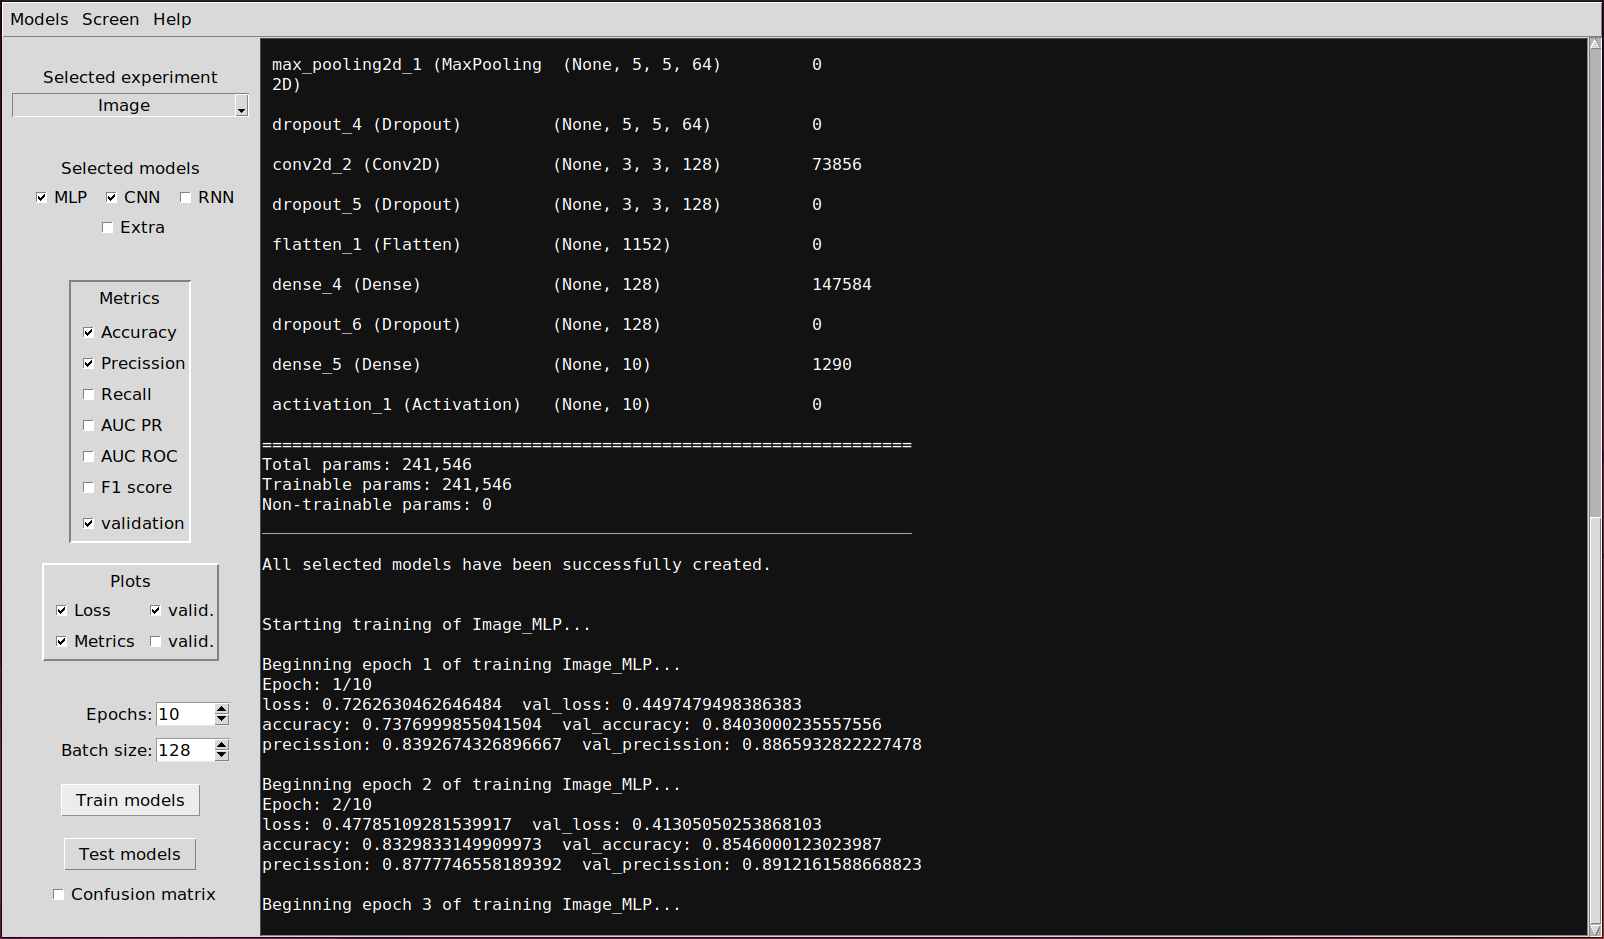
\includegraphics[width=\textwidth]{obrazky-figures/GUI_example.png}
    \caption{The experimental application's GUI created using Tkinter.}
    \label{fig:gui-example}
\end{figure}








\chapter{Course and evaluation of the experiments}
\label{course-and-evaluation-of-the-experiments}
The description of each experiment's course starts with a reasoned choice of the batch size, the number of
epochs, and the selected metrics.
The results are then presented, mainly in the form of generated graphs, and some conclusions are made
based on the visible trends and patterns.
Each dataset had been only split into train and test subsets, with the test set also being used as the validation
set, and validation happening every training epoch, so testing a model at any given time is expected to yield results
very similar to the validation phase of its most recent training epoch.

This chapter is split into sections \ref{Tabular-data-classification}, \ref{image-data-classification} and
\ref{sequential-data-classification}, corresponding to the individual experiments.
All measured values are rounded to four (training) or eight (testing) decimal places
for the sake of the readability.




\section{Tabular data classification}
\label{Tabular-data-classification}
%Why batch size, which metrics etc.
This experiment could be considered an anomaly detection problem, since we're more focused on detecting a rare event
(less commonly occurring positive class) and less concerned about the nagative cases.
For this reason, most of the available metrics (see figure \ref{fig:gui-example}) had been measured, as they're mostly
based on precision and recall,
both of which are very relevant for this kind of problem.
The only metric to be left out is area under the ROC curve,
as ROC curves can sometimes be misleadingly optimistic in imbalanced problems, while misclassifying most of the
minority class cases.

A rule of thumb for choosing the number of epochs for training on data with extracted features is to
start with the number of features multiplied by 3 (in this case $50*3=150$). After some experimentation with larger numbers of epochs, I decided to settle on this value as the visible trends didn't really change and the
improvement progress stagnated heavily after that point.
The batch size had been set to 256, which should be large enough to average out random fluctuations given
the size of the dataset.
\pagebreak


\subsection{Results}
First, the graphs of the training metrics' progress are shown and described, then the testing phase is presented
via the confusion matrices and a table of the measured metrics.

\subsubsection{Training phase}
%training and testing - graphs, matrix, table etc.
\begin{figure}[!h]
    \centering
    \begin{minipage}{0.48\textwidth}
        \centering
        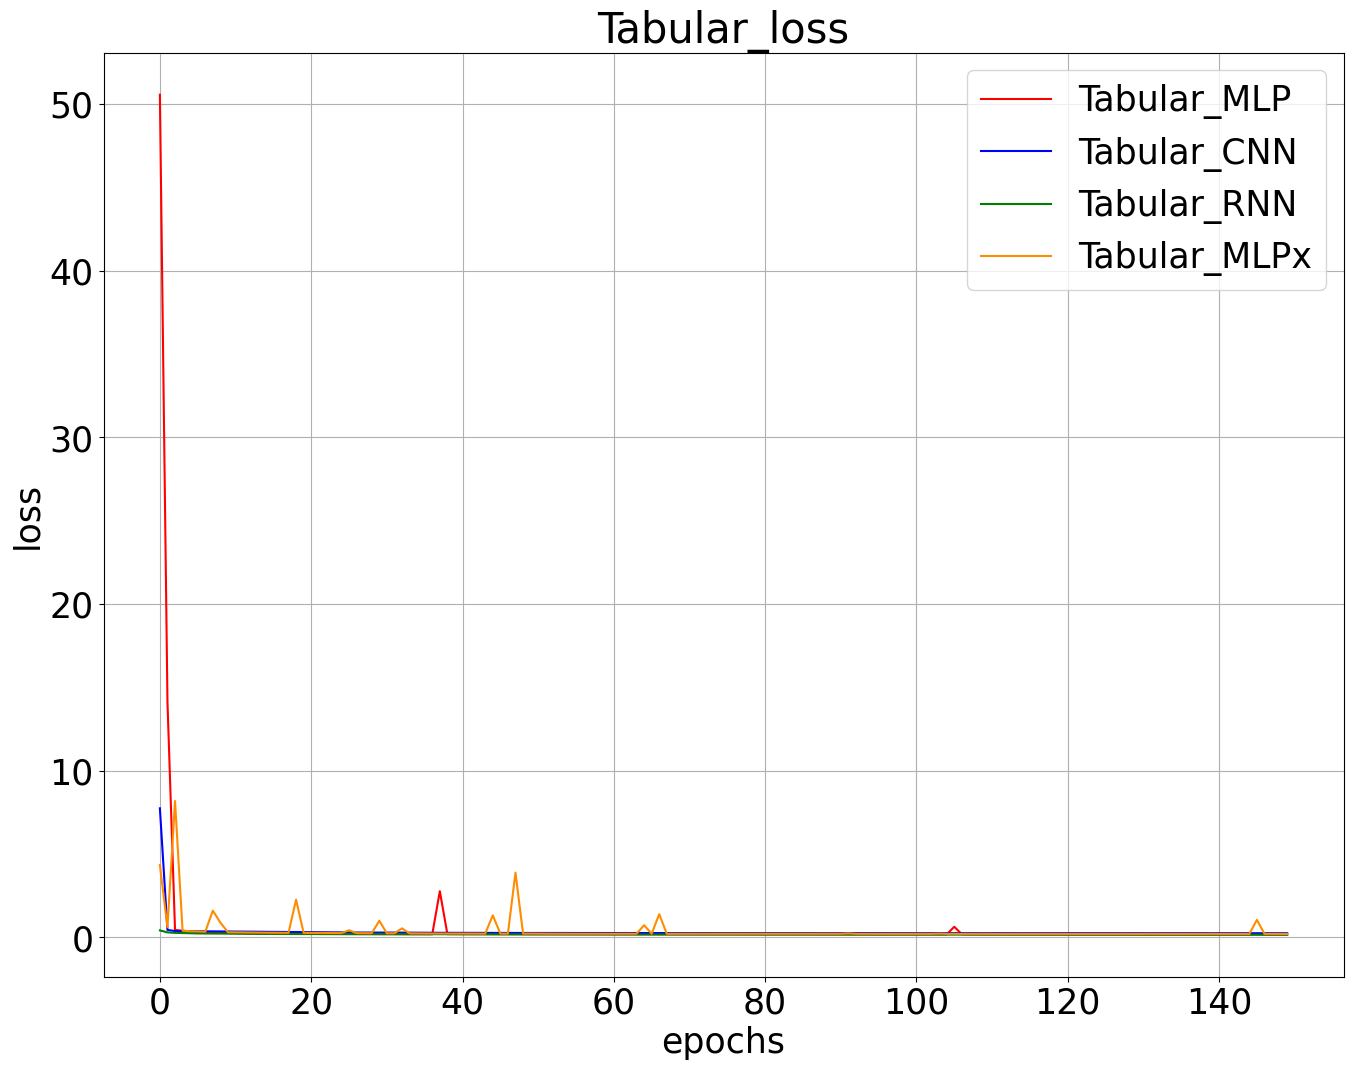
\includegraphics[width=\linewidth]{obrazky-figures/Tabular_experiment/loss_2023-03-23_15:04:45.png}
        \caption{Training loss progress.}
        \label{graph-tabular-loss}
    \end{minipage}\hfill
    \begin{minipage}{0.48\textwidth}
        \centering
        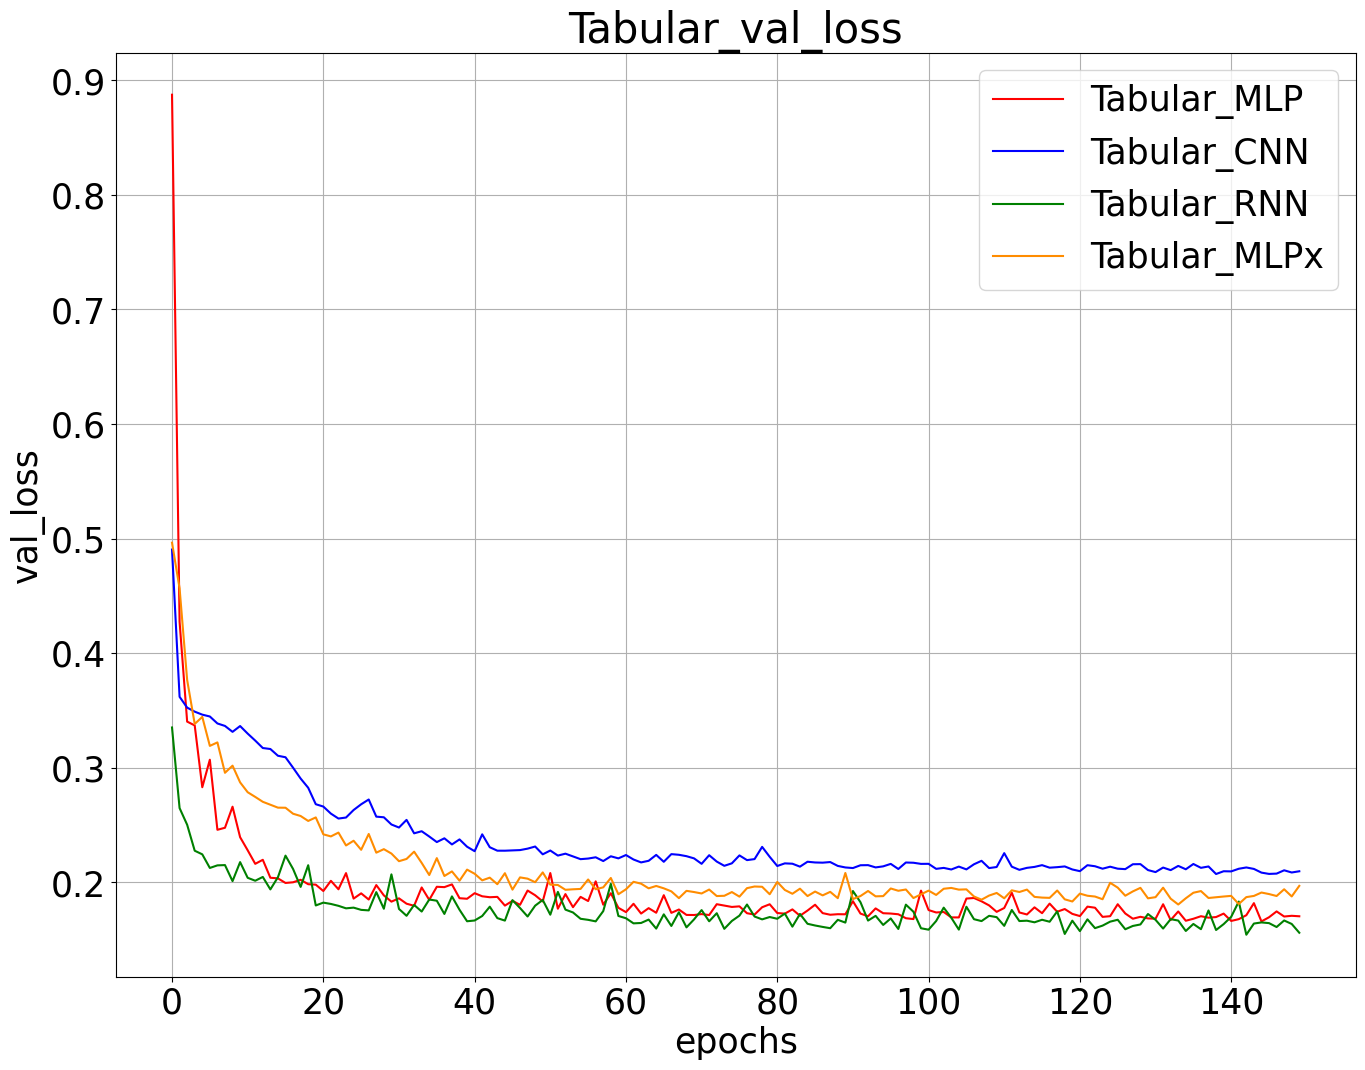
\includegraphics[width=\linewidth]{obrazky-figures/Tabular_experiment/val_loss_2023-03-23_15:04:45.png}
        \caption{Validation loss progress.}
        \label{graph-tabular-val_loss}
    \end{minipage}
\end{figure}
Since the graph of training loss (figure \ref{graph-tabular-loss}) is very ``zoomed out'', most of the following information was derived from
the training logs. The most prominent progress happened in the first four epochs, where all models
reached training loss of about 0.4.
\texttt{Tabular\_CNN} ended up being the worst with 0.2535 loss after the entire training, while the best performing
was surprisingly \texttt{Tabular\_RNN} with loss of 0.1635, closely followed by \texttt{Tabular\_MLP} (0.1774).
Somewhere in the middle ended up \texttt{Tabular\_MLPx} with 0.2093 loss.

All models seem to generalize very well, as quite unexpectedly, most models' validation loss (figure
\ref{graph-tabular-val_loss}) was about 0.4 to 0.8 lower than
its training loss. \texttt{Tabular\_RNN} took this trend even further with an impressive 0.2096 validation loss.
The relative performance of the models is consistent in terms of training and validation loss.
\pagebreak


\begin{figure}[!ht]
    \centering
    \begin{minipage}{0.48\textwidth}
        \centering
        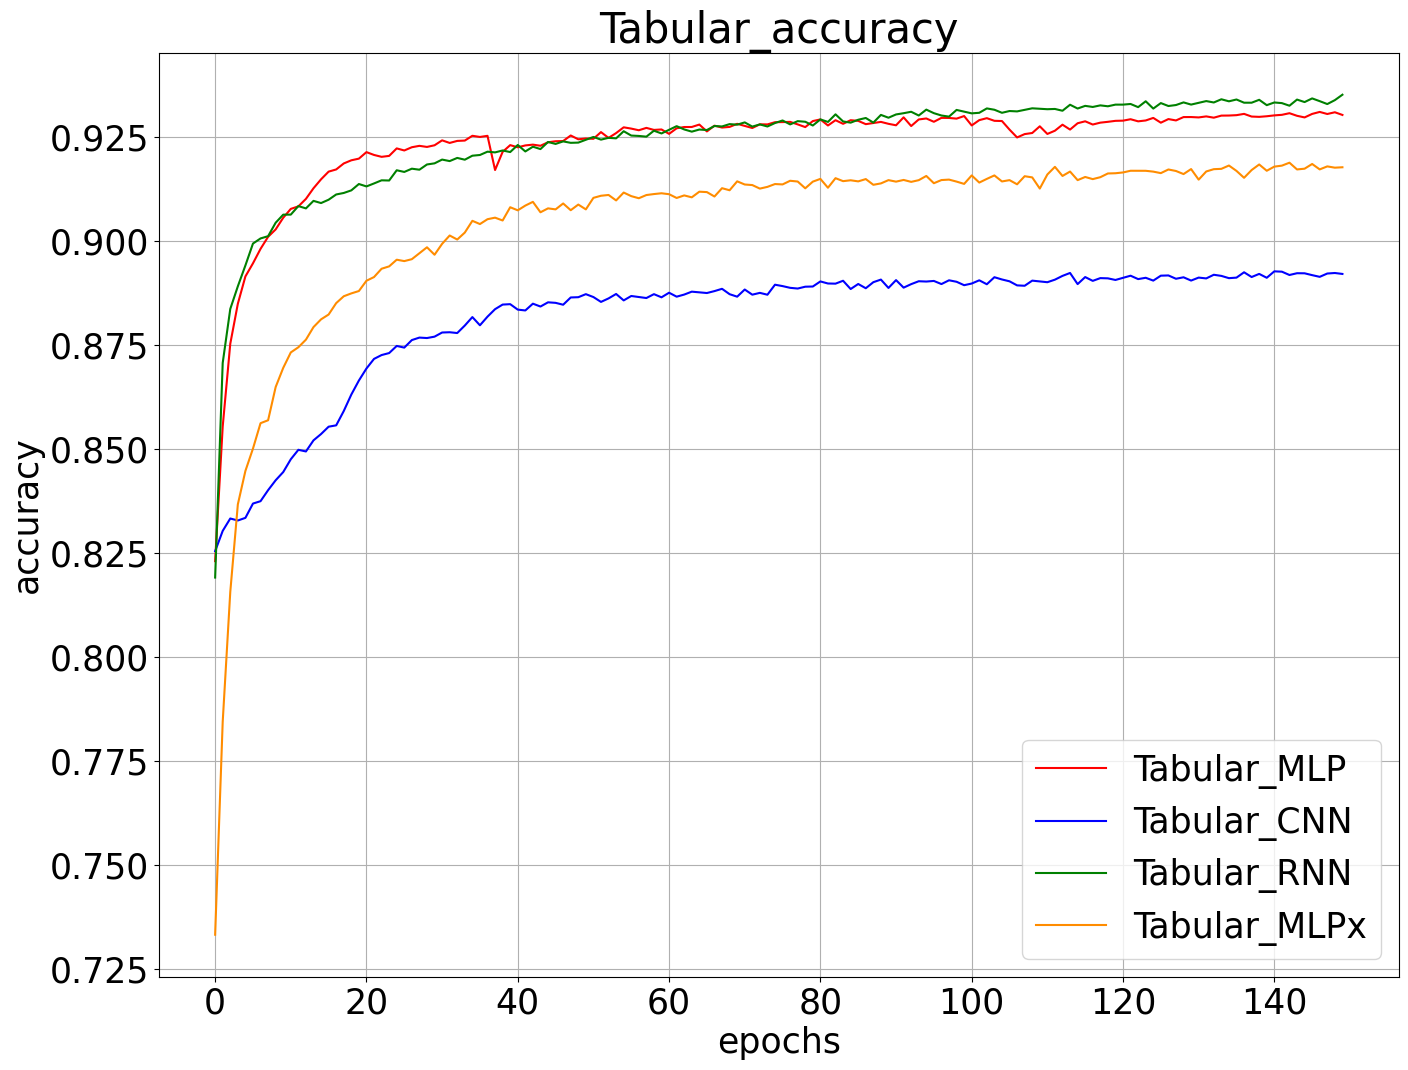
\includegraphics[width=\linewidth]{obrazky-figures/Tabular_experiment/accuracy_2023-03-23_15:04:45.png}
        \caption{Training accuracy progress.}
        \label{graph-tabular-accuracy}
    \end{minipage}\hfill
    \begin{minipage}{0.48\textwidth}
        \centering
        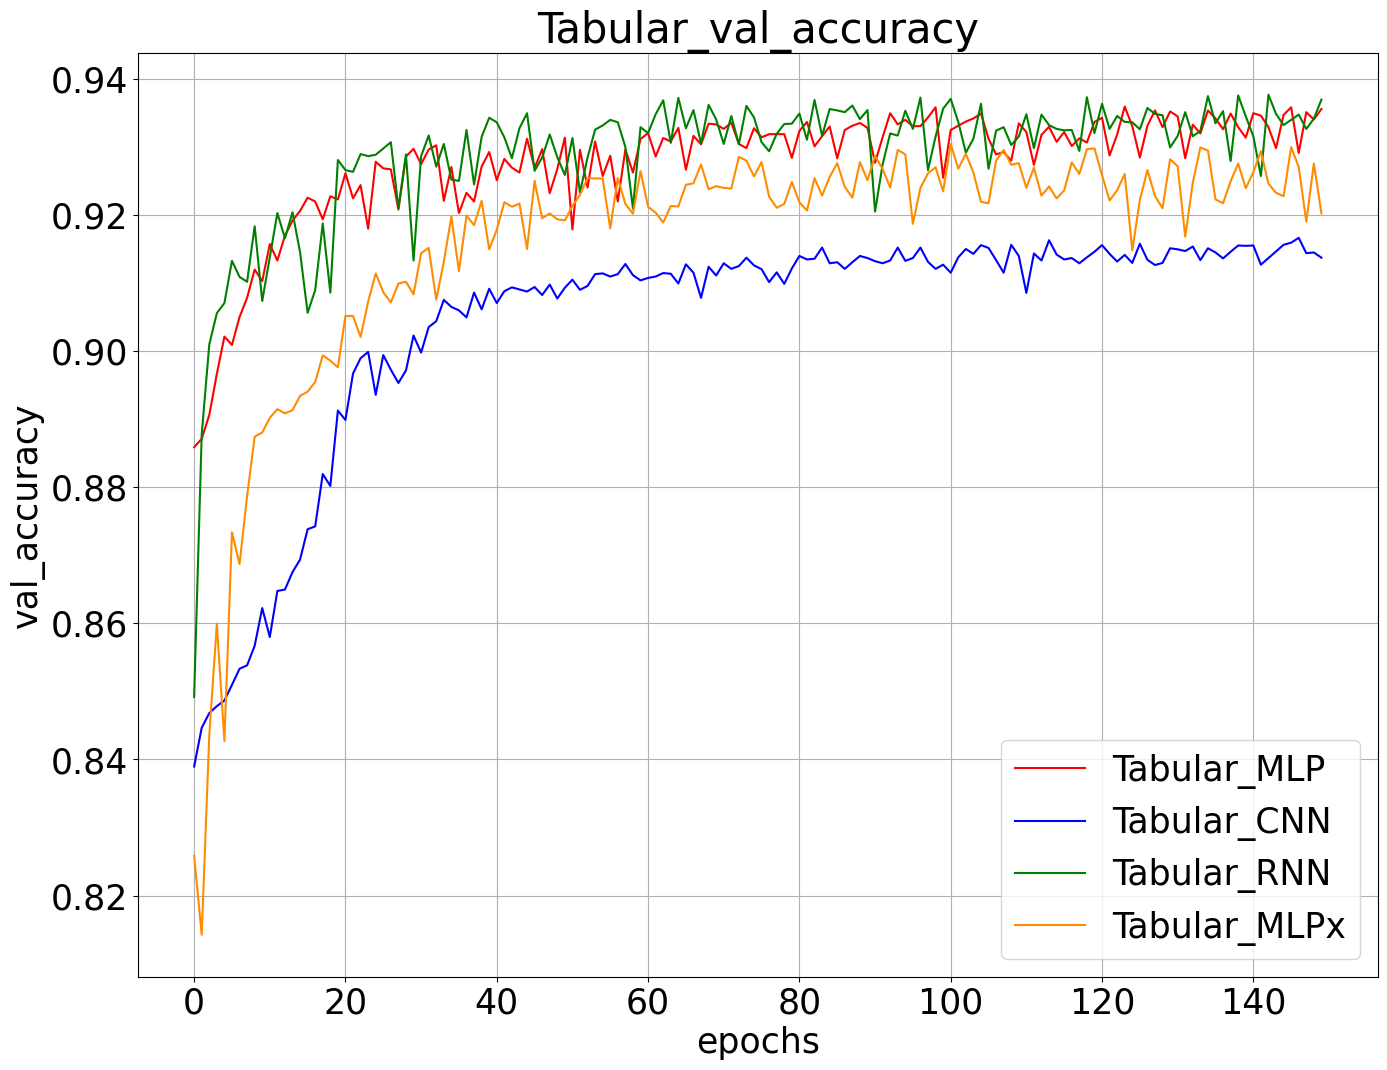
\includegraphics[width=\linewidth]{obrazky-figures/Tabular_experiment/val_accuracy_2023-03-23_15:04:45.png}
        \caption{Validation accuracy progress.}
        \label{graph-tabular-val_accuracy}
    \end{minipage}
\end{figure}
All models reached at least 0.875 training (figure \ref{graph-tabular-accuracy}) and 0.9 validation (figure
\ref{graph-tabular-val_accuracy}) accuracy in the first 20 epochs, and drastically slowed down their improvement after
that point.
Even though \texttt{Tabular\_MLP} performed the best in the beginning, it was, again, closely outperformed by
\texttt{Tabular\_RNN}, which ended up with 0.935 training and 0.9369 validation accuracy.
The worst performing was again \texttt{Tabular\_CNN} with 0.892 training and 0.9137 validation accuracy.
Just as was the case with loss, all models showed better validation performance than training performance
and the models' relative performance is basically the same.


\begin{figure}[!h]
    \centering
    \begin{minipage}{0.48\textwidth}
        \centering
        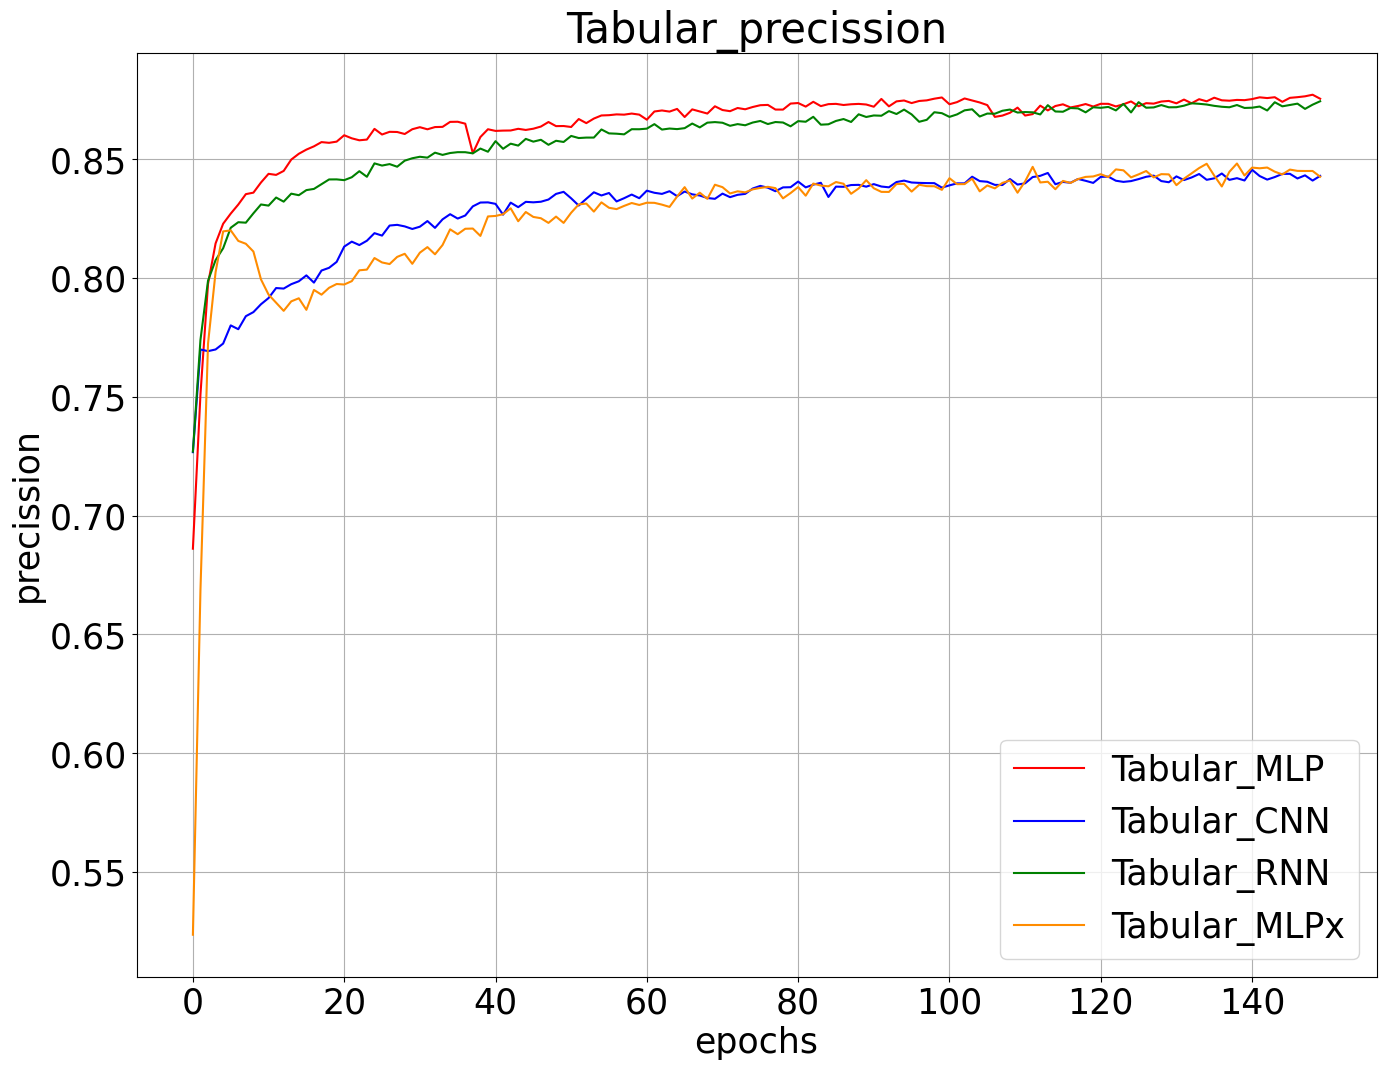
\includegraphics[width=\linewidth]{obrazky-figures/Tabular_experiment/precission_2023-03-23_15:04:45.png}
        \caption{Training precision progress.}
        \label{graph-tabular-precision}
    \end{minipage}\hfill
    \begin{minipage}{0.48\textwidth}
        \centering
        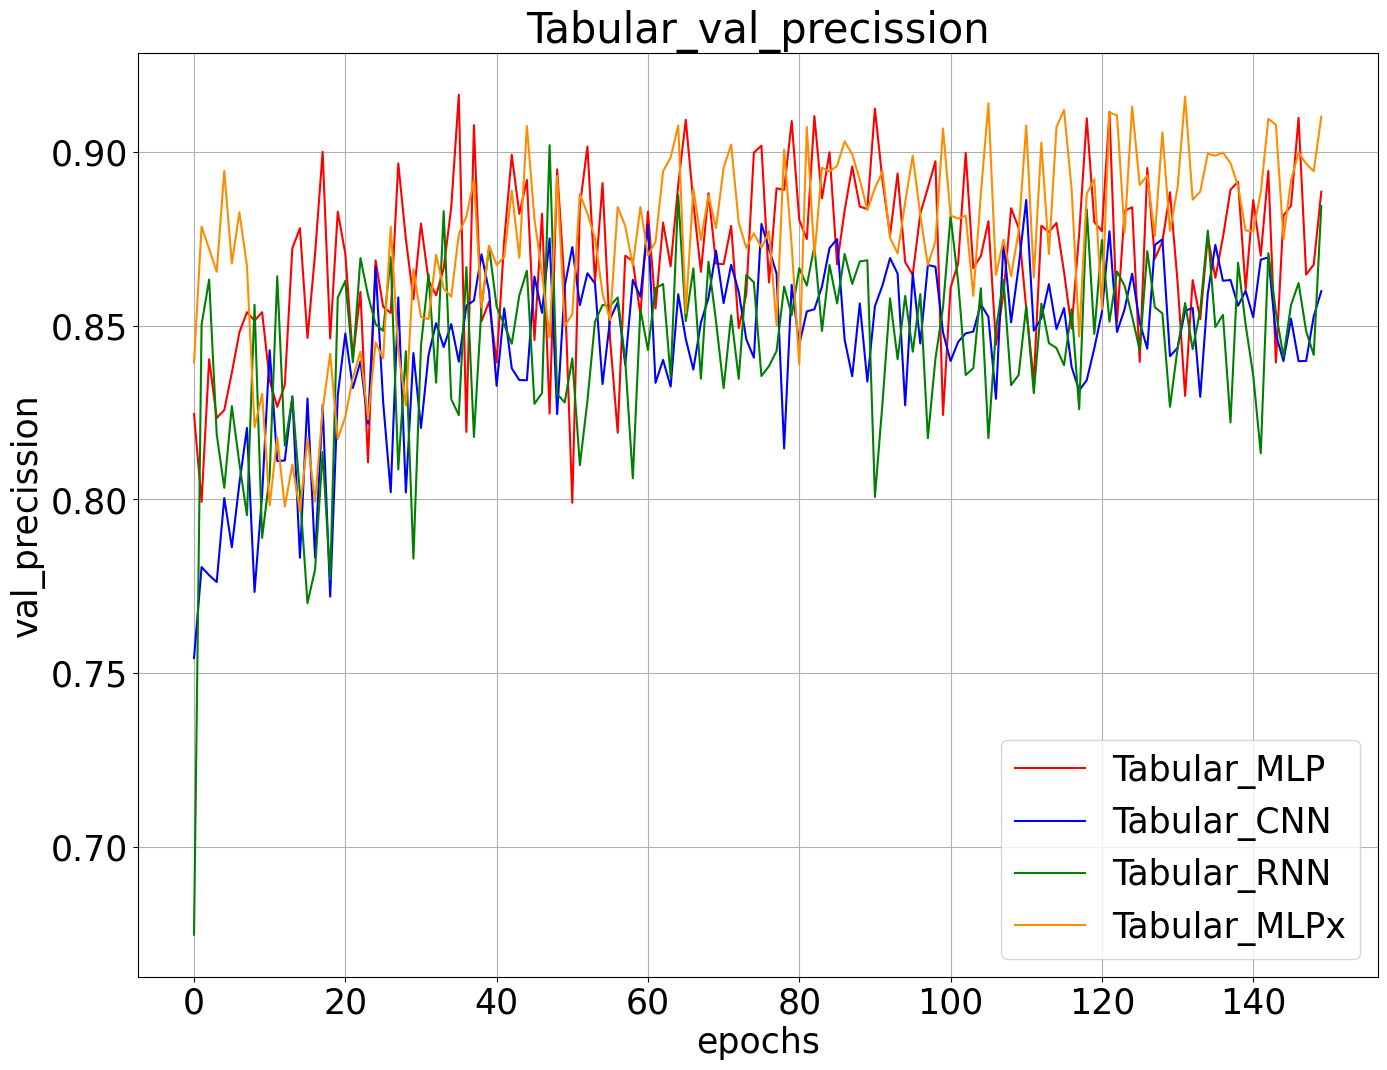
\includegraphics[width=\linewidth]{obrazky-figures/Tabular_experiment/val_precission_2023-03-23_15:04:46.png}
        \caption{Validation precision progress.}
        \label{graph-tabular-val_precision}
    \end{minipage}
\end{figure}
In both cases, precision split the models into two pairs. In the case of training precision (figure
\ref{graph-tabular-precision}), the better pair consists of \texttt{Tabular\_RNN} and \texttt{Tabular\_MLP},
which reached 0.8755 precision, while the worse pair converged to a value about 0.035 lower,
\texttt{Tabular\_MLPx} reaching the worst training precision of only 0.8426.

Interestingly enough, in validation precision (figure \ref{graph-tabular-val_precision}, whose graph seems to be quite noisy
because of many spikes),
\texttt{Tabular\_MLPx} was, along with \texttt{Tabular\_MLP}, part of the better performing pair,
and the only model to end up with above 0.9 precision, with a value of 0.9102.
It also proved itself as the most consistent model, as its spikes didn't dip as low as the ones of all the other models.
\pagebreak


\begin{figure}[!ht]
    \centering
    \begin{minipage}{0.48\textwidth}
        \centering
        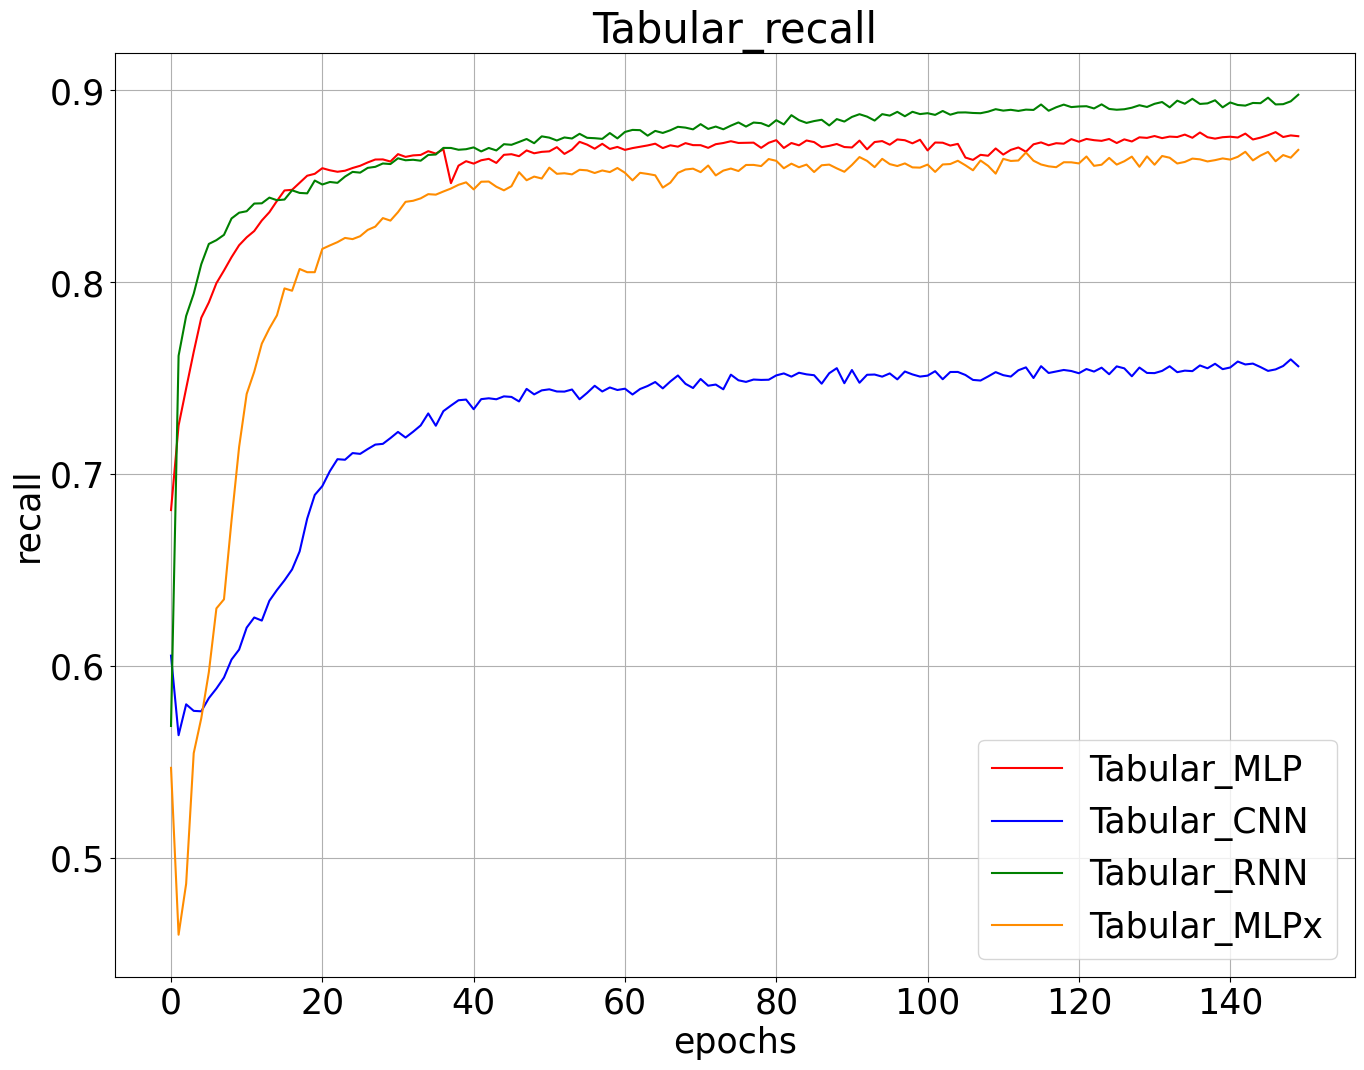
\includegraphics[width=\linewidth]{obrazky-figures/Tabular_experiment/recall_2023-03-23_15:04:45.png}
        \caption{Training recall progress.}
        \label{graph-tabular-recall}
    \end{minipage}\hfill
    \begin{minipage}{0.48\textwidth}
        \centering
        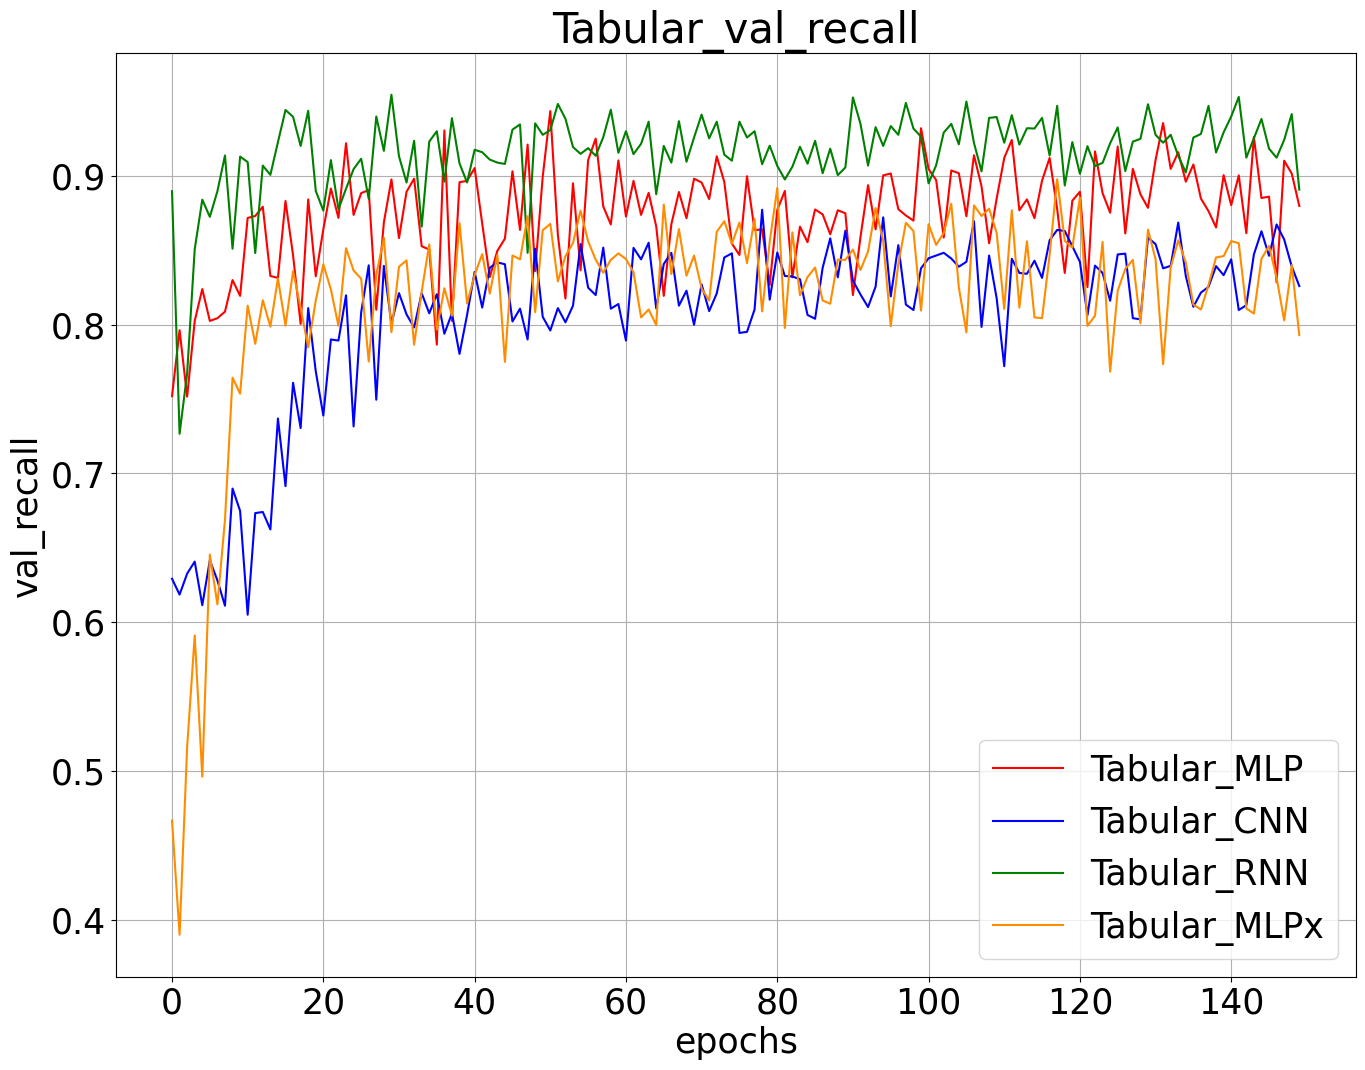
\includegraphics[width=\linewidth]{obrazky-figures/Tabular_experiment/val_recall_2023-03-23_15:04:46.png}
        \caption{Validation recall progress.}
        \label{graph-tabular-val_recall}
    \end{minipage}
\end{figure}
Both training (figure \ref{graph-tabular-recall}) and validation (figure \ref{graph-tabular-val_recall}) recall were visibly
dominated by \texttt{Tabular\_RNN}, reaching
values of 0.8979 and 0.8908 respectively, although the validation recall dipped in the last epoch and
peaked at 0.9546 during the 30th epoch. Not too far behind were the MLPs, both reaching about $0.87 \pm 0.005$ training recall.
Horrible performance can be seen from \texttt{Tabular\_CNN}, which started stagnating at a value of about 0.75,
although it tightly outperformed \texttt{Tabular\_MLPx} in validation, where it also peaked during the 75th epoch
at a more ``respectable'' value of 0.8479.


\begin{figure}[!h]
    \centering
    \begin{minipage}{0.48\textwidth}
        \centering
        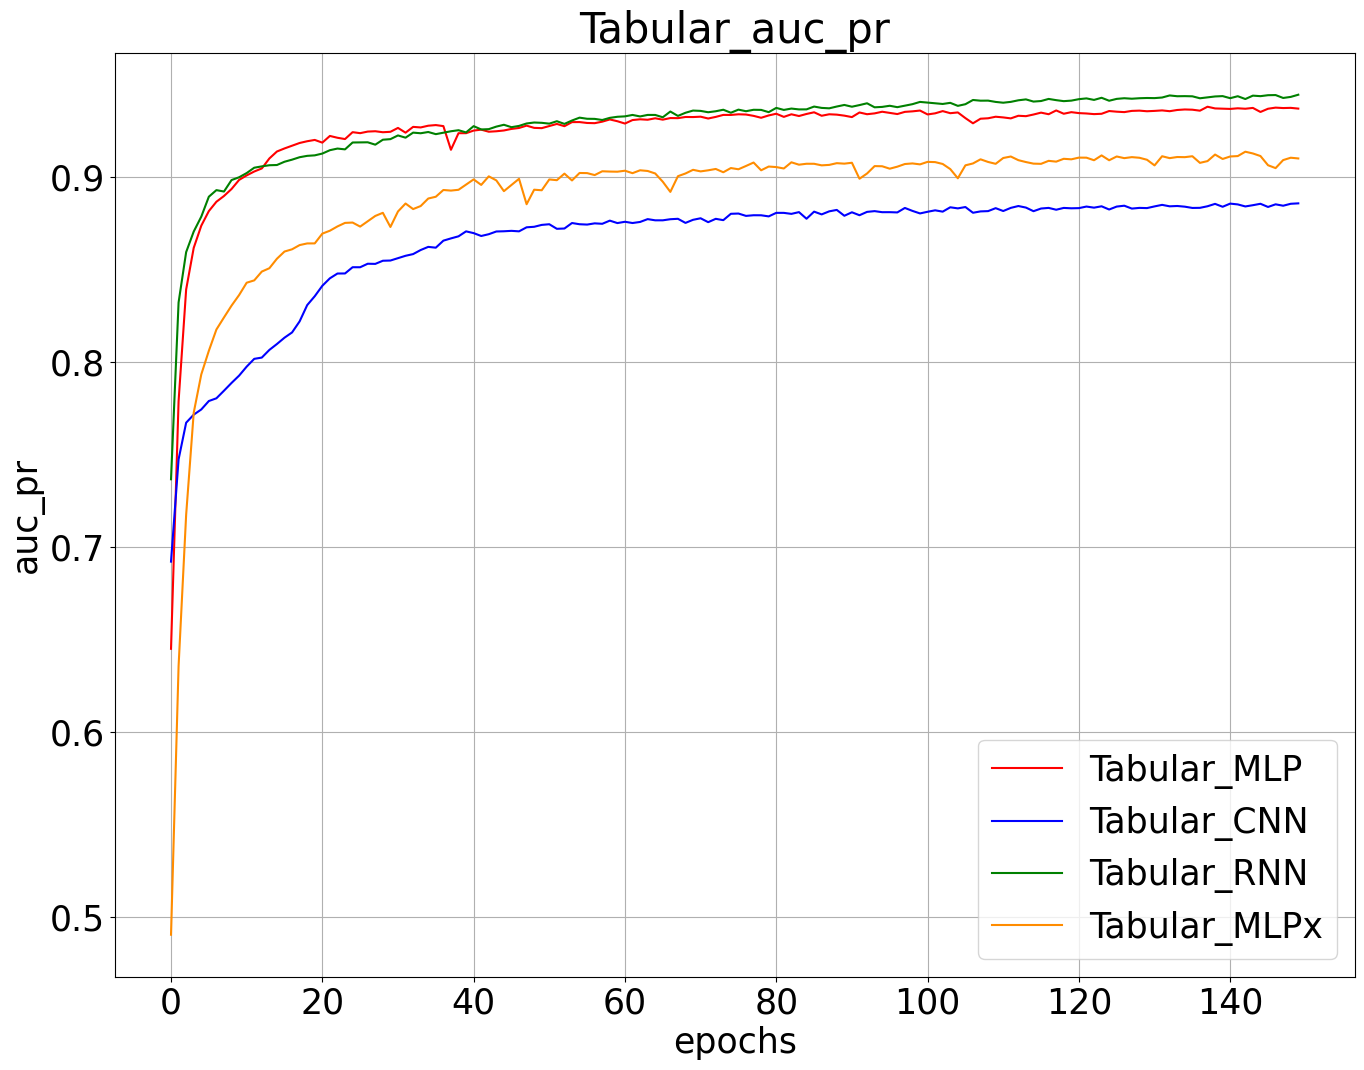
\includegraphics[width=\linewidth]{obrazky-figures/Tabular_experiment/auc_pr_2023-03-23_15:04:45.png}
        \caption{Training AUC PR progress.}
        \label{graph-tabular-auc-pr}
    \end{minipage}\hfill
    \begin{minipage}{0.48\textwidth}
        \centering
        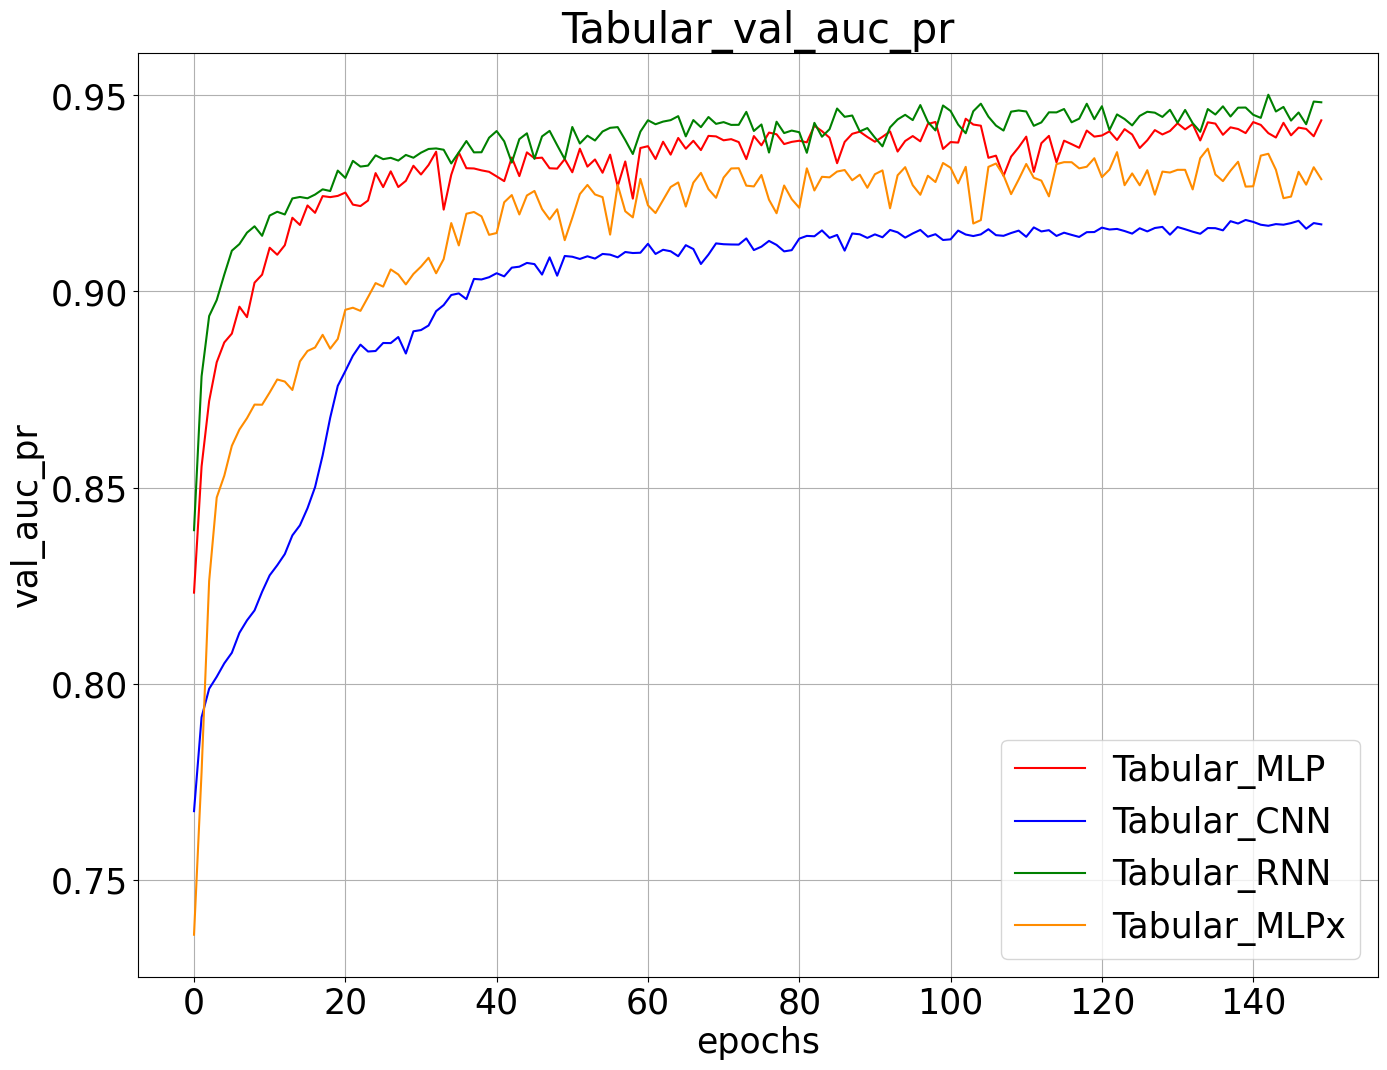
\includegraphics[width=\linewidth]{obrazky-figures/Tabular_experiment/val_auc_pr_2023-03-23_15:04:46.png}
        \caption{Validation AUC PR progress.}
        \label{graph-tabular-val_auc-pr}
    \end{minipage}
\end{figure}
The AUC PR (Area unded the precision-recall curve) graphs look very similar to the accuracy graphs.
This applies to the AUC PR graph (figure \ref{graph-tabular-auc-pr}) compared to figure \ref{graph-tabular-accuracy},
as well as the validation AUC PR graph (figure \ref{graph-tabular-val_auc-pr}) compared to figure
\ref{graph-tabular-val_accuracy}.
The best performer, \texttt{Tabular\_RNN}, reached 0.9442 training and 0.9482 validation AUC PR in the last epoch,
while the worst one, \texttt{Tabular\_CNN}, only reached values of 0.8855 and 0.9171 respectively.
\pagebreak


\begin{figure}[!ht]
    \centering
    \begin{minipage}{0.48\textwidth}
        \centering
        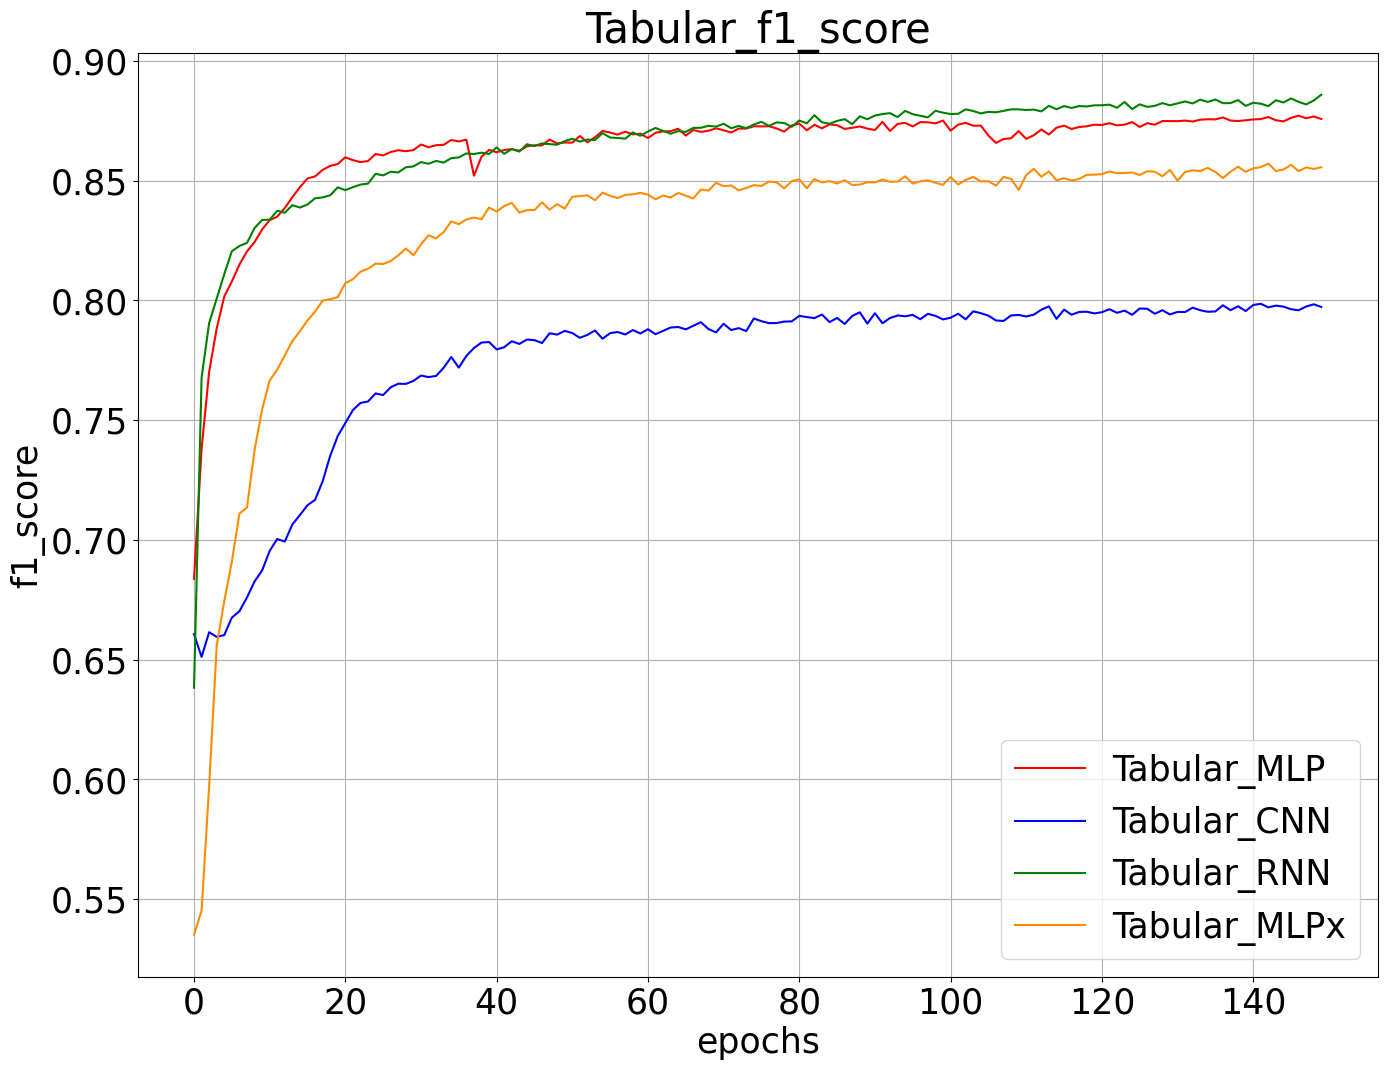
\includegraphics[width=\linewidth]{obrazky-figures/Tabular_experiment/f1_score_2023-03-23_15:04:46.png}
        \caption{Training $F_1$ score progress.}
        \label{graph-tabular-f1}
    \end{minipage}\hfill
    \begin{minipage}{0.48\textwidth}
        \centering
        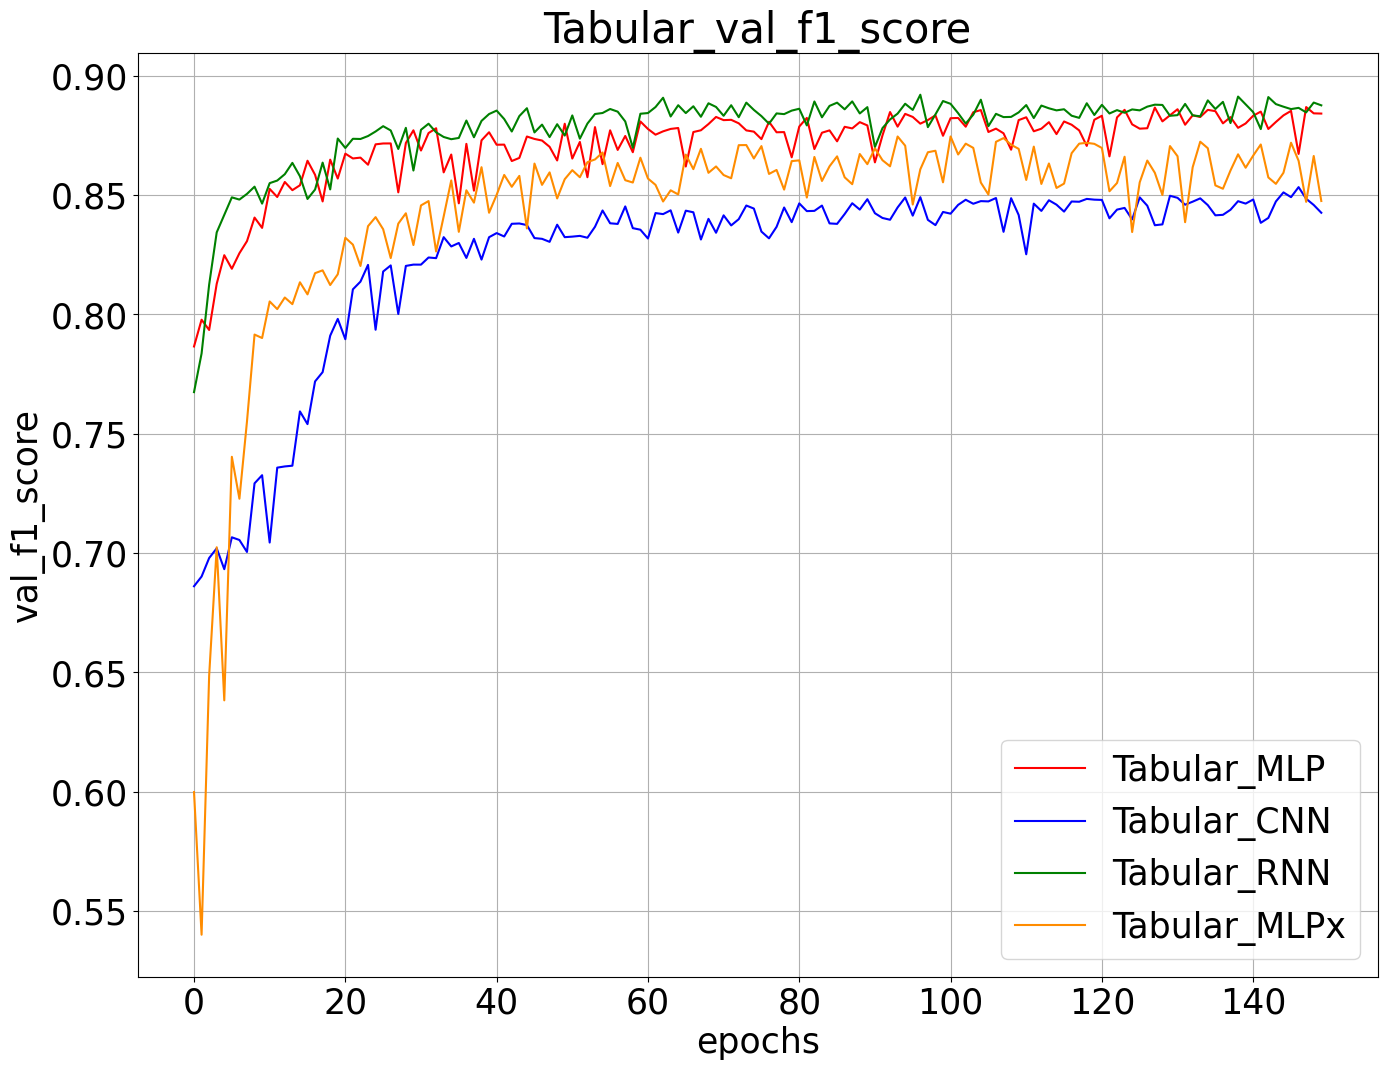
\includegraphics[width=\linewidth]{obrazky-figures/Tabular_experiment/val_f1_score_2023-03-23_15:04:46.png}
        \caption{Validation $F_1$ score progress.}
        \label{graph-tabular-val_f1}
    \end{minipage}
\end{figure}
Measures of the $F_1$ score are, again, very similar to both accuracy and AUC PR. The most visible difference is the
training $F_1$ score (figure \ref{graph-tabular-f1}) of \texttt{Tabular\_CNN}, as $F_1$ score strongly punishes the trade-off between
precision and recall, in which \texttt{Tabular\_CNN} struggled a lot (see figure \ref{graph-tabular-recall}).
Overall, the highest training $F_1$ score (0.8859) in the last epoch was, again, obtained by \texttt{Tabular\_RNN}, while
\texttt{Tabular\_CNN} only reached a value of 0.7973.

Results of the validation F1 score (figure \ref{graph-tabular-val_f1}) seem more balanced, as in the last epoch,
\texttt{Tabular\_RNN} measured 0.8876 and \texttt{Tabular\_CNN} measured 0.8426, which is not too far behind
given the difference of their training $F_1$ scores.


\subsubsection{Testing phase}
Please note that this is the only experiment where the test set was resampled from the dataset between training
and testing, so it doesn't directly correspond to the validation set.

\begin{figure}[!h]
    \centering
    \begin{minipage}{0.48\textwidth}
        \centering
        \captionsetup{justification=centering}
        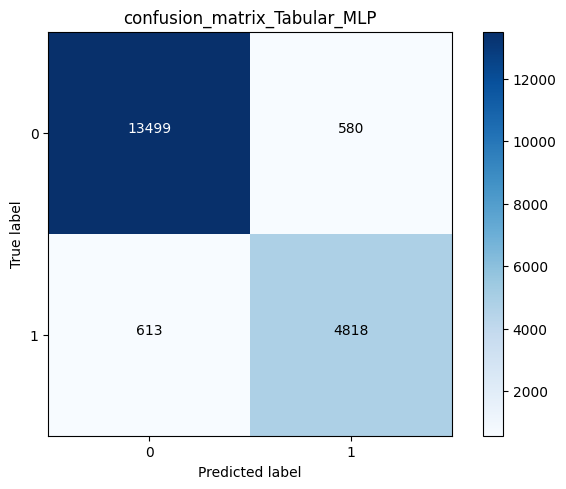
\includegraphics[width=\linewidth]{obrazky-figures/Tabular_experiment/confusion_matrix_Tabular_MLP_2023-03-25_14:48:21.png}
        \caption{Confusion matrix of \texttt{Tabular\_MLP}.}
        \label{graph-tabular-cm-mlp}
    \end{minipage}\hfill
    \begin{minipage}{0.48\textwidth}
        \centering
        \captionsetup{justification=centering}
        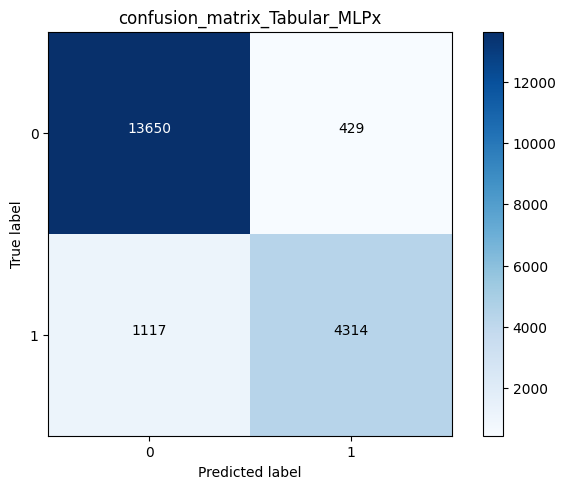
\includegraphics[width=\linewidth]{obrazky-figures/Tabular_experiment/confusion_matrix_Tabular_MLPx_2023-03-25_14:48:25.png}
        \caption{Confusion matrix of \texttt{Tabular\_MLPx}.}
        \label{graph-tabular-cm-mlpx}
    \end{minipage}
\end{figure}
The confusion matrices of the two MLPs (figures \ref{graph-tabular-cm-mlp} and \ref{graph-tabular-cm-mlpx})
reveal that \texttt{Tabular\_MLP}, with it's lesser depth and wider layers, was more prone to predicting
the less occurring positive label than its deeper counterpart, especially when the actual label was positive.
Its positive predictions make up 27.6679~\%, while
\texttt{Tabular\_MLPx}'s make up only 24.3106~\%
of all predicted labels (the actual occurrence of the positive class in the test set was 27.837~\%).


\begin{figure}[!h]
    \centering
    \begin{minipage}{0.48\textwidth}
        \centering
        \captionsetup{justification=centering}
        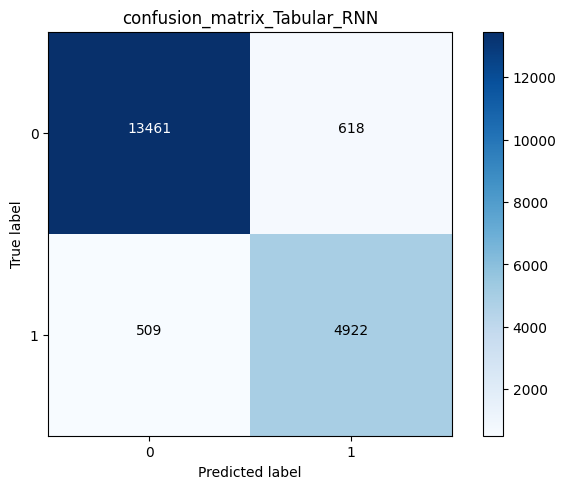
\includegraphics[width=\linewidth]{obrazky-figures/Tabular_experiment/confusion_matrix_Tabular_RNN_2023-03-25_14:48:24.png}
        \caption{Confusion matrix of \texttt{Tabular\_RNN}.}
        \label{graph-tabular-cm-rnn}
    \end{minipage}
    \begin{minipage}{0.48\textwidth}
        \centering
        \captionsetup{justification=centering}
        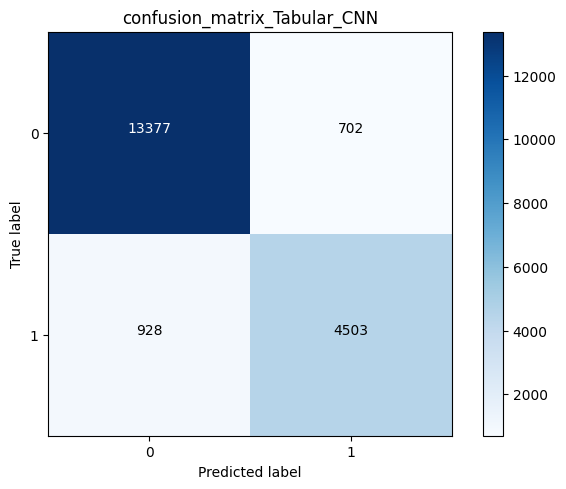
\includegraphics[width=\linewidth]{obrazky-figures/Tabular_experiment/confusion_matrix_Tabular_CNN_2023-03-25_14:48:23.png}
        \caption{Confusion matrix of \texttt{Tabular\_CNN}.}
        \label{graph-tabular-cm-cnn}
    \end{minipage}\hfill
\end{figure}
As its confusion matrix (figure \ref{graph-tabular-cm-rnn}) shows, \texttt{Tabular\_RNN} improved
on \texttt{Tabular\_MLP}'s amount of TPs by 104, for the cost of only 38 more FPs.
Its positive predictions make up 28.3957~\%, making it the only overly optimistic model, as well as the best
performing.

Even though \texttt{Tabular\_CNN} (figure \ref{graph-tabular-cm-cnn}) counts less FNs than
\texttt{Tabular\_MLPx}, the count is still unimpressive as well as its FP count, making it the worst
overall performing model in terms of rounded predictions, with a 26.6786\% positive prediction rate.


\begin{table}[!h]
\centering
\begin{tabular}{|c|c|c|c|c|}
    \cline{1-5}
    \textbf{Metric} & \texttt{Tabular\_MLP} & \texttt{Tabular\_CNN} & \texttt{Tabular\_RNN} & \texttt{Tabular\_MLPx} \\
    \cline{1-5}
    Loss & 0.16712075 & 0.20510150 & 0.14320368 & 0.19452372 \\
    \cline{1-5}
    Accuracy & 0.93885189 & 0.92765248 & 0.93251324 & 0.92957455 \\
    \cline{1-5}
    Precision & 0.89255279 & 0.87909085 & 0.88230193 & 0.88848990 \\ 
    \cline{1-5}
    Recall & 0.88712943 & 0.85812926 & 0.87417912 & 0.85421652 \\
    \cline{1-5}
    AUC PR & 0.94987130 & 0.93610001 & 0.94286144 & 0.93956620 \\
    \cline{1-5}
    F1 score & 0.88983280 & 0.86848354 & 0.87822169 & 0.87101614 \\
    \cline{1-5}
\end{tabular}
\caption{Loss and metrics values measured during the testing phase of the tabular data experiment.}
\label{table:tabular-test}
\end{table}
Table \ref{table:tabular-test} shows all values measured in testing.
Not that surprisingly, \texttt{Tabular\_MLP} beat \texttt{Tabular\_MLPx} by every metric (and loss).
What's interesting is that while \texttt{Tabular\_RNN} measured lower loss than \texttt{Tabular\_MLP}, it got
slightly outperformed by every single metric.
The overall worst performing model seems to be \texttt{Tabular\_CNN}, mainly due to its low precision and recall
(low AUC PR and $F_1$
score are direct consequences of that). Even though \texttt{Tabular\_MLPx} measured very slightly lower recall, it ``redeemed''
itself by the measured precision.


\subsection{Conclusion}
The comparison of MLPs with more width (number of neurons in a layer), represented by \texttt{Tabular\_MLP},
and those with more depth (more layers), represented by \texttt{Tabular\_MLPx}, is pretty straightforward in this case,
as  \texttt{Tabular\_MLP} outperformed the latter by almost every measure, although usually not by a too large margin.
It can be concluded that at least on this scale and in this kind of problem, an increase in width should precede
stacking more layers, that also leads to slower training and unnecessary complexity.

As for the other NN types, \texttt{Tabular\_RNN} proved itself as a very competent alternative to MLPs for when
the features measure the same kind of phenomena, happening just at different time or space points.
Not only were its results very impressive, but also consistent, and the model seemed to learn very quickly.
The 1D convolutional network, \texttt{Tabular\_CNN}, performed poorly compared to the other models, but
a very possible explanation might be that its bottleneck was the small convolutional kernel size (3),
limiting its ability to recognize global patterns, as opposed to the MLPs, working only globally,
and \texttt{Tabular\_RNN}, which was able to store much more context in its recurrent memory.
It is very much possible that increasing the kernel size would've had a strong positive impact on the model's
performance, as 1D convolutional networks are very commonly used for handling problems of similar nature.




\section{Image data classification}
\label{image-data-classification}
The only metric to be measured in this balanced multi-class image classification experiment is
accuracy, as the other available metrics (see figure \ref{fig:gui-example}) would have to be measured
with respect to a specific class, but in this case, all classes share an equal importance
(any important characteristics of the trained models will still be visible in the confusion matrices).

The number of epochs had been set to 200, which is quite a lot, but some interesting changes in the graphs
were happening around the 150th epoch. The batch size had been kept at 32, as small mini-batches are very
common for computer vision problems.


\subsection{Results}
Again, first the training results and then the testing results are presented.
\pagebreak

\subsubsection{Training phase}
\begin{figure}[!ht]
    \centering
    \begin{minipage}{0.48\textwidth}
        \centering
        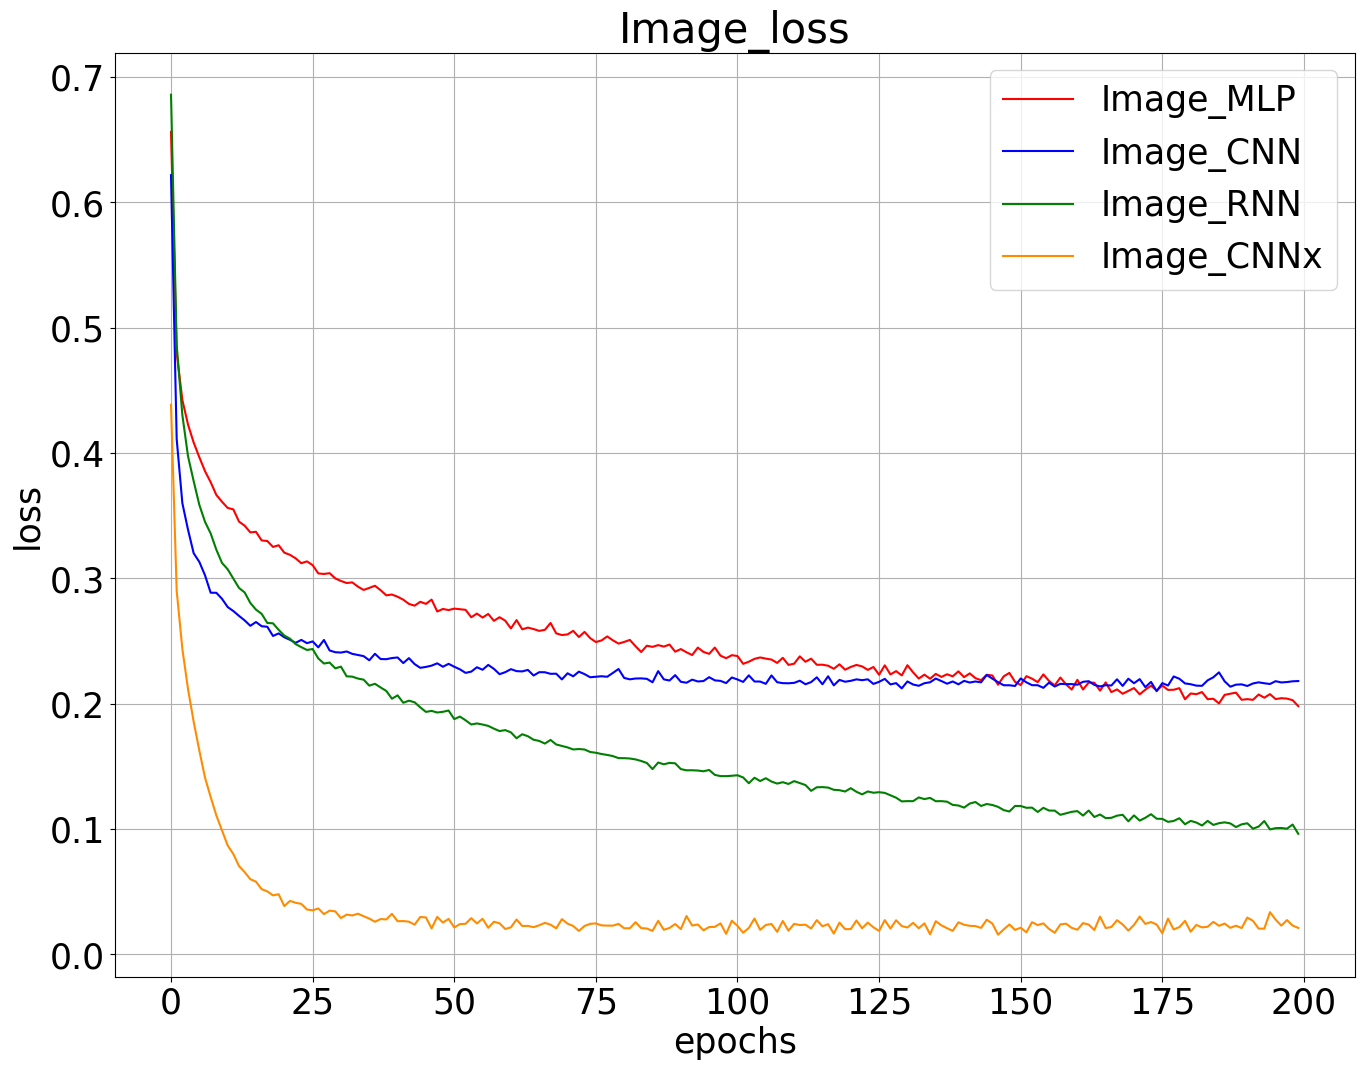
\includegraphics[width=\linewidth]{obrazky-figures/Image_experiment/loss_2023-03-27_13:08:08.png}
        \caption{Training loss progress.}
        \label{graph-image-loss}
    \end{minipage}\hfill
    \begin{minipage}{0.48\textwidth}
        \centering
        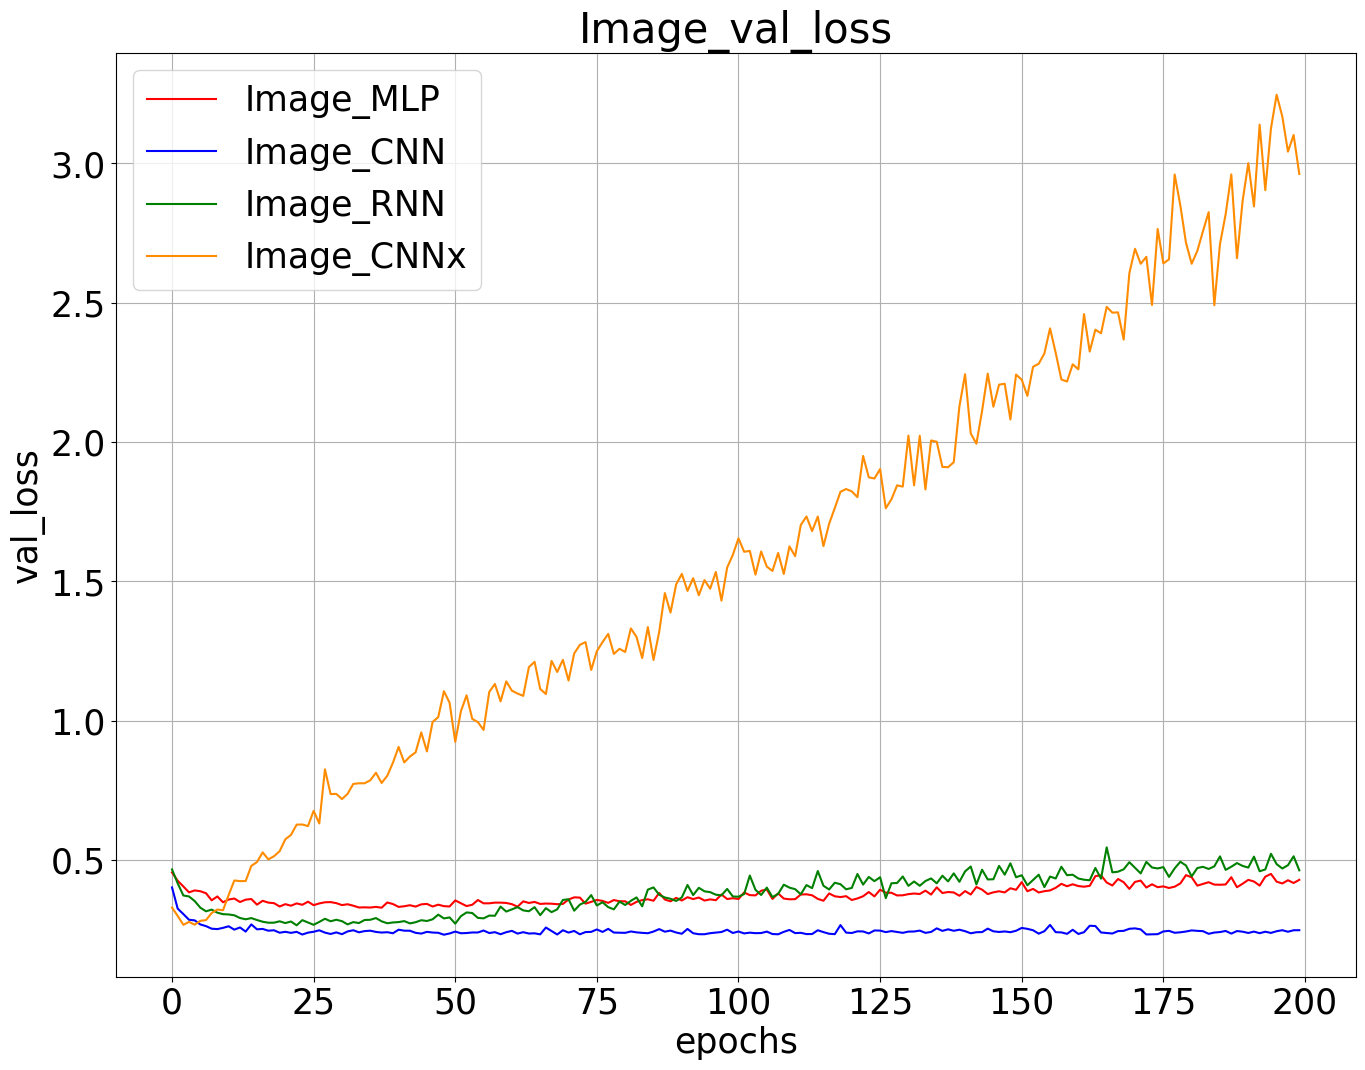
\includegraphics[width=\linewidth]{obrazky-figures/Image_experiment/val_loss_2023-03-27_13:08:08.png}
        \caption{Validation loss progress.}
        \label{graph-image-val_loss}
    \end{minipage}
\end{figure}
First thing to notice in the training (figure \ref{graph-image-loss}) and validation (figure \ref{graph-image-val_loss})
loss graphs is how quickly \texttt{Image\_CNNx}, the only unregularized model, reached training loss of only about 0.025
(0.021 in the final epoch). This is obviously a case of strong overfitting, as its validation loss was steadily
increasing, peaking at 3.246 in the 196th epoch, and would probably keep increasing even more if the training continued.
In the contrary, the training loss of \texttt{Image\_CNN}, which shares the same architecture but heavily regularized,
basically converged to values of about 0.215. This paid off well, as its validation loss reached values
as small as 0.2326 (49th epoch) very quickly, outperforming the other models effortlessly.

The battle between \texttt{Image\_RNN} and \texttt{Image\_MLP} ended up in favor of the former,
as in the final epoch, \texttt{Image\_RNN} reached training loss about twice as low (0.0961 vs 0.198)
for the cost of only about 10 \% higher validation loss (0.4636 vs 0.4295).


\begin{figure}[!h]
    \centering
    \begin{minipage}{0.48\textwidth}
        \centering
        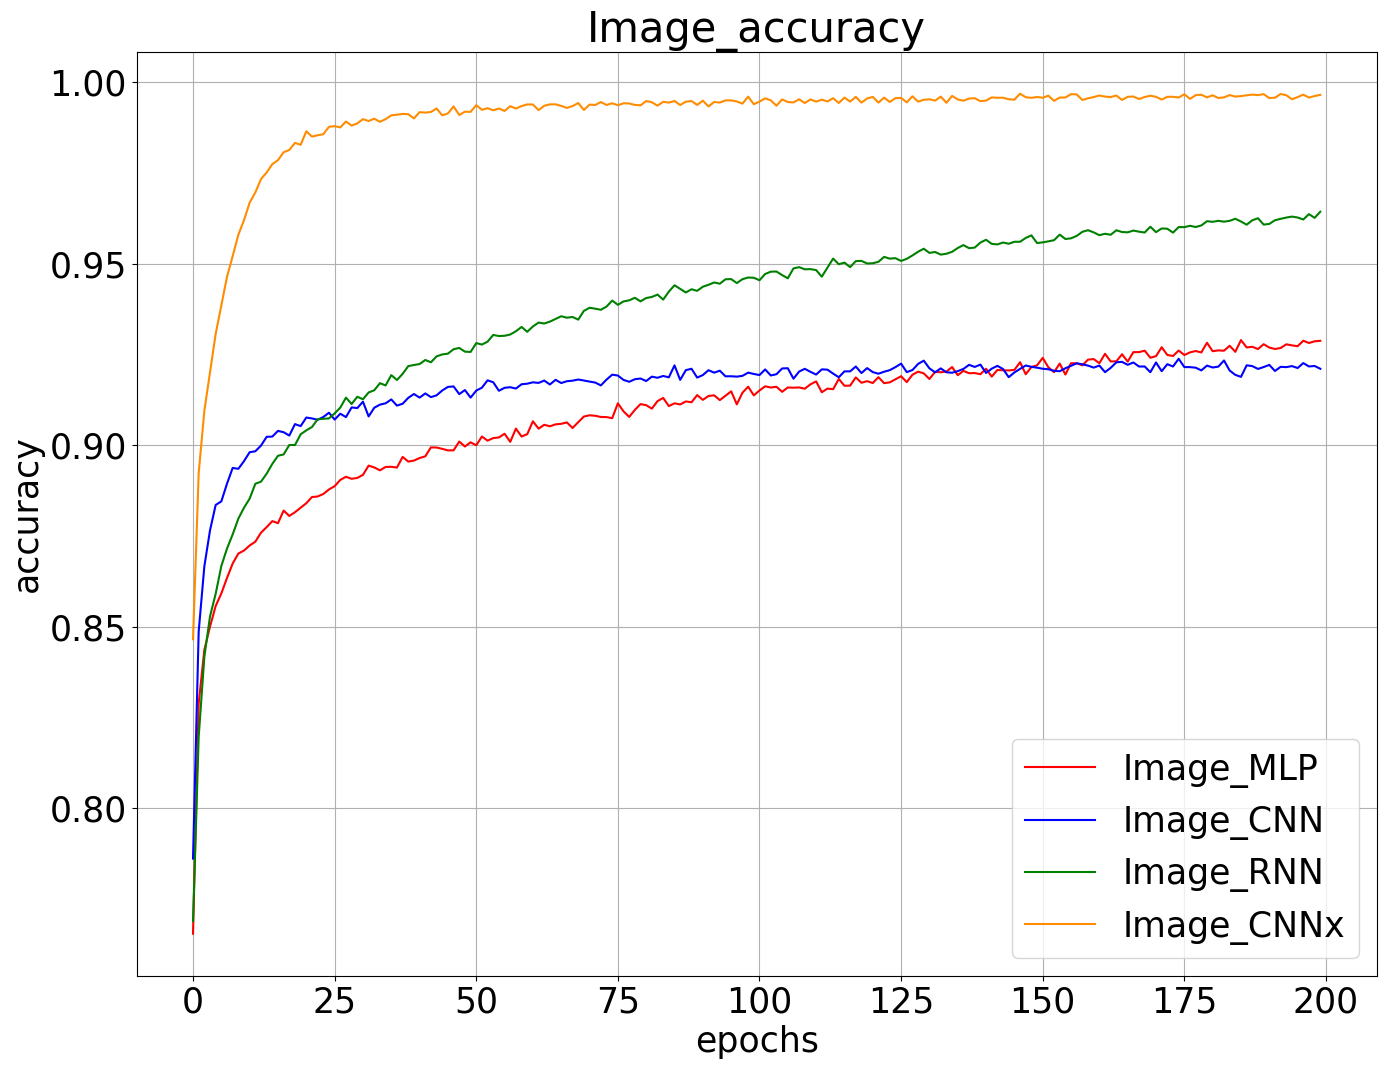
\includegraphics[width=\linewidth]{obrazky-figures/Image_experiment/accuracy_2023-03-27_13:08:08.png}
        \caption{Training accuracy progress.}
        \label{graph-image-accuracy}
    \end{minipage}\hfill
    \begin{minipage}{0.48\textwidth}
        \centering
        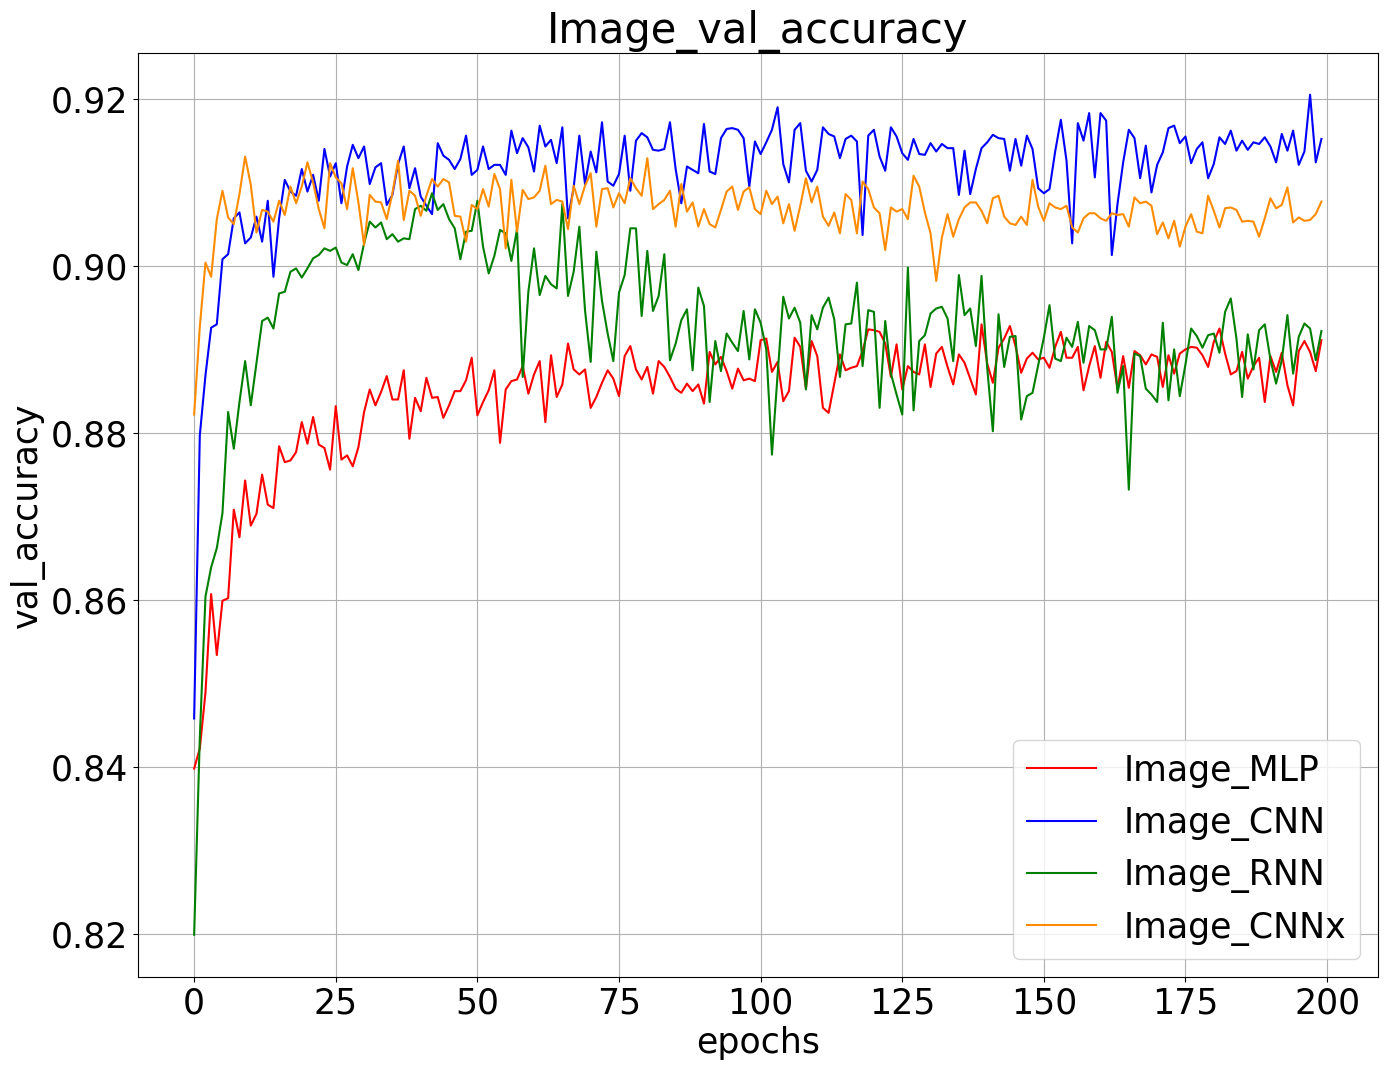
\includegraphics[width=\linewidth]{obrazky-figures/Image_experiment/val_accuracy_2023-03-27_13:08:09.png}
        \caption{Validation accuracy progress.}
        \label{graph-image-val_accuracy}
    \end{minipage}
\end{figure}
The unregularized \texttt{Image\_CNNx} seems to had reached training accuracy (figure \ref{graph-image-accuracy}) of around 0.99
(peaking at 0.9968 during the 147th epoch) extremely quickly. Just as was the case with loss, the second most
accurate model was \texttt{Image\_RNN}, with a training accuracy of 0.9643 in the last epoch.
The main CNN representative, \texttt{Image\_CNN}, plateaud very quicky when reaching values of around 0.92, and it even
got outperformed by \texttt{Image\_MLP} at about the 150th epoch and onwards.

When it comes to validation accuracy (figure \ref{graph-image-val_accuracy}),
\texttt{Image\_CNN} proved itself as the best, although its performance
doesn't seem great enough to excuse the poor training performance, given that it may had been intuitively expected
to perform the best. It ended up at 0.9152 (last epoch), but \texttt{Image\_CNNx} was really close behind with a value
of 0.9077. This was really unexpected, as one would assume the accuracy would decrease much quicker, complementing the loss
increase due to overfitting, but it seemed to be almost unaffected.
At about the 45th epoch, \texttt{Image\_RNN} started showing obvious signs of overfitting, as its validation accuracy
went from around 0.905 down to around 0.89, more or less matching \texttt{Image\_MLP}, which was the worst
performing model in terms of accuracy.


\subsubsection{Testing phase}
\begin{figure}[!h]
    \centering
    \begin{minipage}{0.48\textwidth}
        \centering
        \captionsetup{justification=centering}
        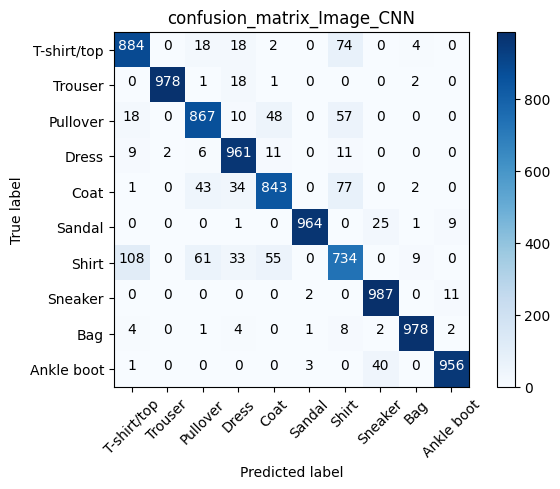
\includegraphics[width=\linewidth]{obrazky-figures/Image_experiment/confusion_matrix_Image_CNN_2023-03-27_21:34:30.png}
        \caption{Confusion matrix of \texttt{Image\_CNN}.}
        \label{graph-image-cm-cnn}
    \end{minipage}\hfill
    \begin{minipage}{0.48\textwidth}
        \centering
        \captionsetup{justification=centering}
        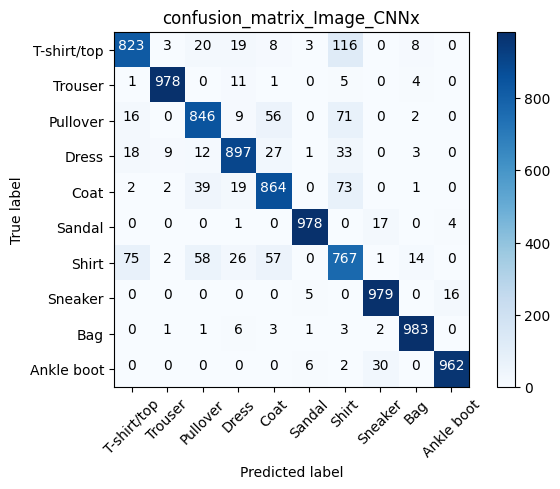
\includegraphics[width=\linewidth]{obrazky-figures/Image_experiment/confusion_matrix_Image_CNNx_2023-03-27_21:34:33.png}
        \caption{Confusion matrix of \texttt{Image\_CNNx}.}
        \label{graph-image-cm-cnnx}
    \end{minipage}
\end{figure}
To help interpret the following confusion matrices (figures \ref{graph-image-cm-cnn} and \ref{graph-image-cm-cnnx}),
remember that a perfectly accurate model would have 1,000s on the diagonal and 0s everywhere else, as there
are precisely 1,000 samples of each class in the test set.

Even at first glance, it can be seen that both models seem to have problems with classifying shirts. Not only
are they (mainly \texttt{Image\_CNN}) likely to classify a shirt as something similar, like a T-shirt/top or a coat,
but they (mainly the more overfitted \texttt{Image\_CNNx}) also often tend to classify those as a shirt.
\pagebreak


\begin{figure}[!ht]
    \centering
    \begin{minipage}{0.48\textwidth}
        \centering
        \captionsetup{justification=centering}
        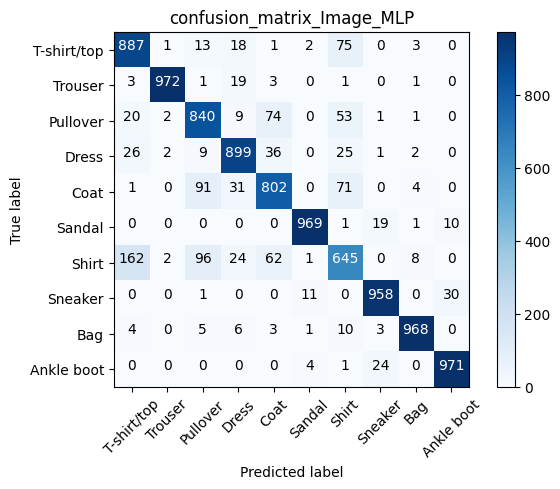
\includegraphics[width=\linewidth]{obrazky-figures/Image_experiment/confusion_matrix_Image_MLP_2023-03-27_21:34:27.png}
        \caption{Confusion matrix of \texttt{Image\_MLP}.}
        \label{graph-image-cm-mlp}
    \end{minipage}\hfill
    \begin{minipage}{0.48\textwidth}
        \centering
        \captionsetup{justification=centering}
        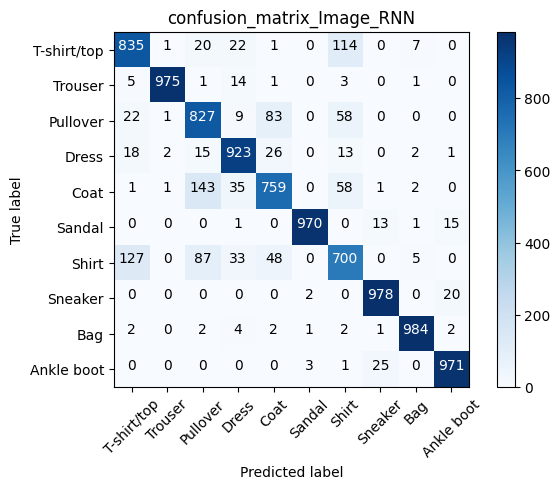
\includegraphics[width=\linewidth]{obrazky-figures/Image_experiment/confusion_matrix_Image_RNN_2023-03-27_21:34:32.png}
        \caption{Confusion matrix of \texttt{Image\_RNN}.}
        \label{graph-image-cm-rnn}
    \end{minipage}
\end{figure}
Similar pattern can be seen in the confusion matrices of the worse performing models (figures \ref{graph-image-cm-mlp}
and \ref{graph-image-cm-rnn}). Even more prominent than in
the previous case is the problem with classifying shirts and coats. \texttt{Image\_MLP} classified only
645 shirts correctly, predicting 162 of them to be a T-shirt/top, and \texttt{Image\_RNN} managed to classify
143 coats as a pullover. When it comes to clothes for the lower body, and accessories, the two models
performed almost as well as the convolutional models (and were slightly better at classifying ankle boots for
some reason).


\begin{table}[!h]
\centering
\begin{tabular}{|c|c|c|c|c|}
    \cline{1-5}
    \textbf{Metric} & \texttt{Image\_MLP} & \texttt{Image\_CNN} & \texttt{Image\_RNN} & \texttt{Image\_CNNx} \\
    \cline{1-5}
    Loss & 0.42950425 & 0.24873139 & 0.46358573 & 2.96167660 \\
    \cline{1-5}
    Accuracy & 0.89109999 & 0.90315002 & 0.89950001 & 0.90154999 \\
    \cline{1-5}
\end{tabular}
\caption{Loss and metrics values measured during the testing phase of the image data experiment.}
\label{table:image-test}
\end{table}
Table \ref{table:image-test} shows almost nothing new. All models seem to perform just about the same in terms
of accuracy, except for \texttt{Tabular\_MLP}, that scored about 0.01 lower than the rest.


\subsection{Conclusion}
The steadily increasing loss of \texttt{Image\_CNNx} was very much expected, but its great test accuracy
was very surprising. This demonstrates that when the data is split uniformly between classes in the train
set and small enough batches are used (smaller batches introduce noise that has a regularizing
effect~\cite{DBLP:journals/corr/abs-1804-07612}),
the negative impacts of overfitting reduce drastically.

I would advise against using MLPs for image classification outside of educational purposes, 
due to their inability to recognize local patterns. Even though the worst performing model,
\texttt{Image\_MLP}, didn't perform that much more poorly than the rest,
keep in mind that the images were very small, grayscale, quite simple, and standardized.

Although not as magnificently as in the tabular experiment (section \ref{image-data-classification}),
RNNs somewhat proved themselves again as a possible viable alternative, this time to CNNs.
But one can wonder how well this scales to more complex problems, as my understanding of \texttt{Image\_RNN}'s
mechanism somewhat reminded me of a barcode scanner, scanning the grayscale image from left to right
in parallel with respect to the rows of pixels (but please take this statement with a grain of salt).
One also has to decide between interpreting rows of pixels as features and columns as timesteps, or the other way
around---this is also dependent on the given problem and should be expected to impact the model's performance.




\section{Sequential data classification}
\label{sequential-data-classification}
Again, the only metric to be measured in this experiment is accuracy, as for the other available metrics (see figure
\ref{fig:gui-example}),
the positive class would have to be the main point of interest (or the class labels could get flipped
to relate the metrics to the negative class), but I figured
it might be a better idea to consider positive and negative movie reviews equally (both the train/test sets
are also perfectly balanced in terms of class distribution).

Given that training these models (especially the RNNs) was more time demanding than the previous experiments,
the training was done over 100 epochs, which should yield results scaled similarly to the previous experiments.
The batch size had been set to 64---an optimal batch size for training LSTM-based models in most cases~\cite{gures_2020}.


\subsection{Results}
Once again, first the training results and then the testing results are presented.

\subsubsection{Training phase}
\begin{figure}[!h]
    \centering
    \begin{minipage}{0.48\textwidth}
        \centering
        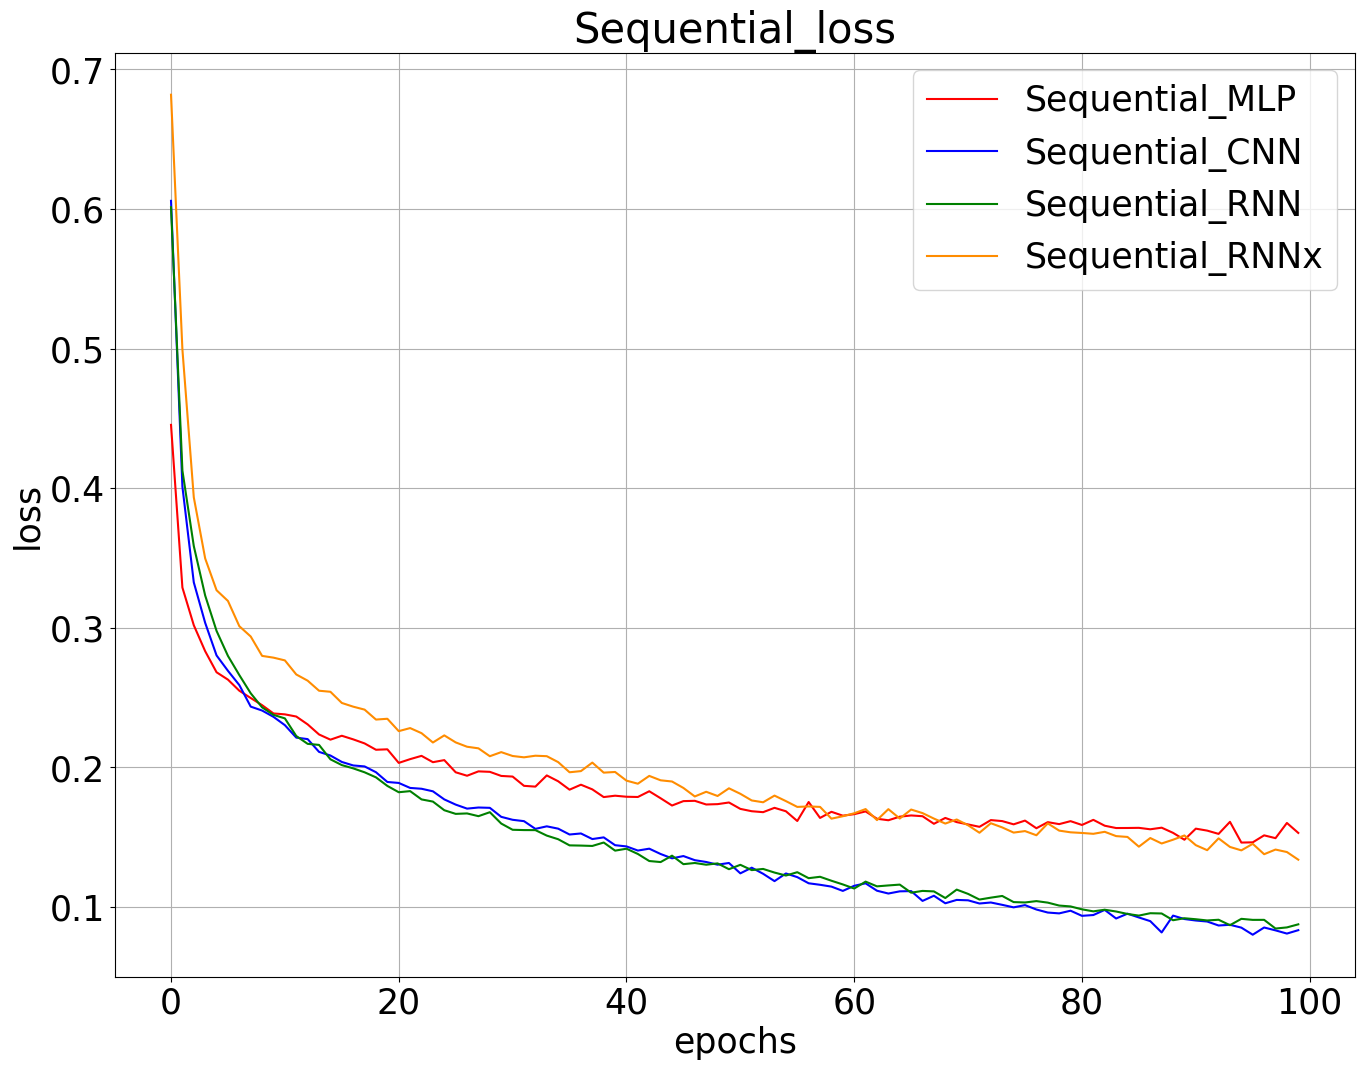
\includegraphics[width=\linewidth]{obrazky-figures/Sequential_experiment/loss_2023-03-29_14:45:07.png}
        \caption{Training loss progress.}
        \label{graph-sequential-loss}
    \end{minipage}\hfill
    \begin{minipage}{0.48\textwidth}
        \centering
        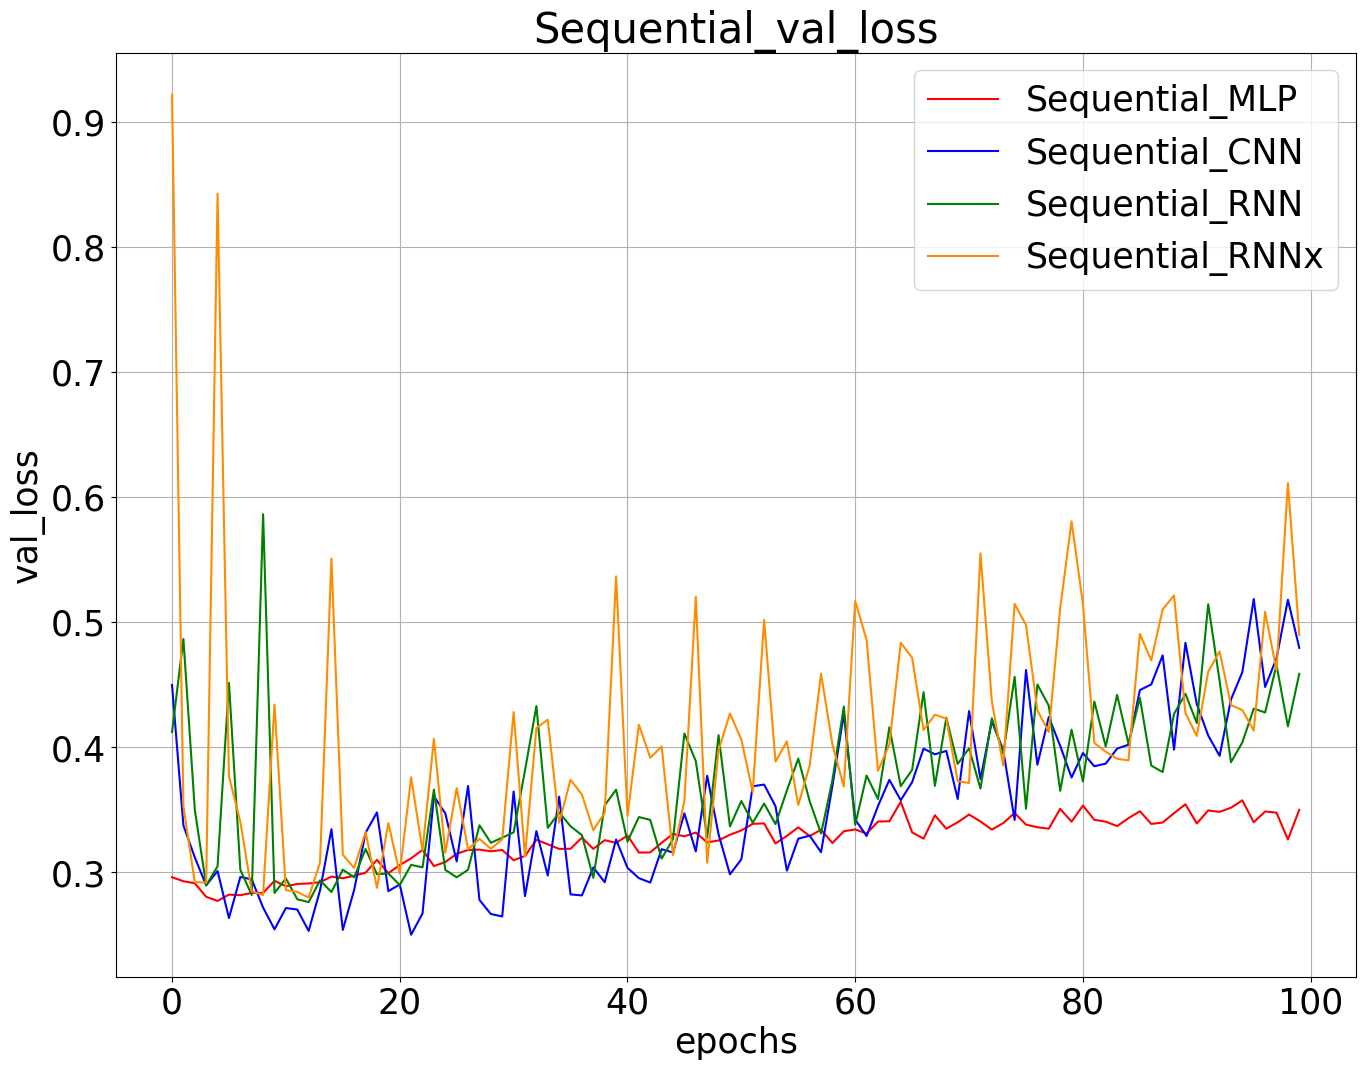
\includegraphics[width=\linewidth]{obrazky-figures/Sequential_experiment/val_loss_2023-03-29_14:45:07.png}
        \caption{Validation loss progress.}
        \label{graph-sequential-val_loss}
    \end{minipage}
\end{figure}
It is clearly visible from both training loss (figure \ref{graph-sequential-loss}) and validation loss (figure
\ref{graph-sequential-val_loss}) graphs, that the more complicated \texttt{Sequential\_RNNx} performed objectively
worse than \texttt{Sequential\_RNN}. Not only did its loss decrease slow down quite early, but there also seems
to be more prominent and unstable overfitting (based on the validation loss).

\texttt{Image\_CNN}'s performance seems to be just as good as \texttt{Sequential\_RNN}'s in both cases.
It measured 0.0834 loss in the last epoch, a bit lower than \texttt{Sequential\_RNN}'s 0.0877, but its validation
loss was hovering around slightly higher values during the last few epochs.
Very surprising was the training performance of \texttt{Sequential\_MLP}, as it performed similarly to \texttt{Sequential\_RNNx} in terms of loss, and much better that all the other models in terms of validation loss
(0.35 during the last epoch, other models measured between 0.45 and 0.49).
This is very impressive, since it only had limited training information available (vectorized words) compared
to the other models (embedded words).


\begin{figure}[!h]
    \centering
    \begin{minipage}{0.48\textwidth}
        \centering
        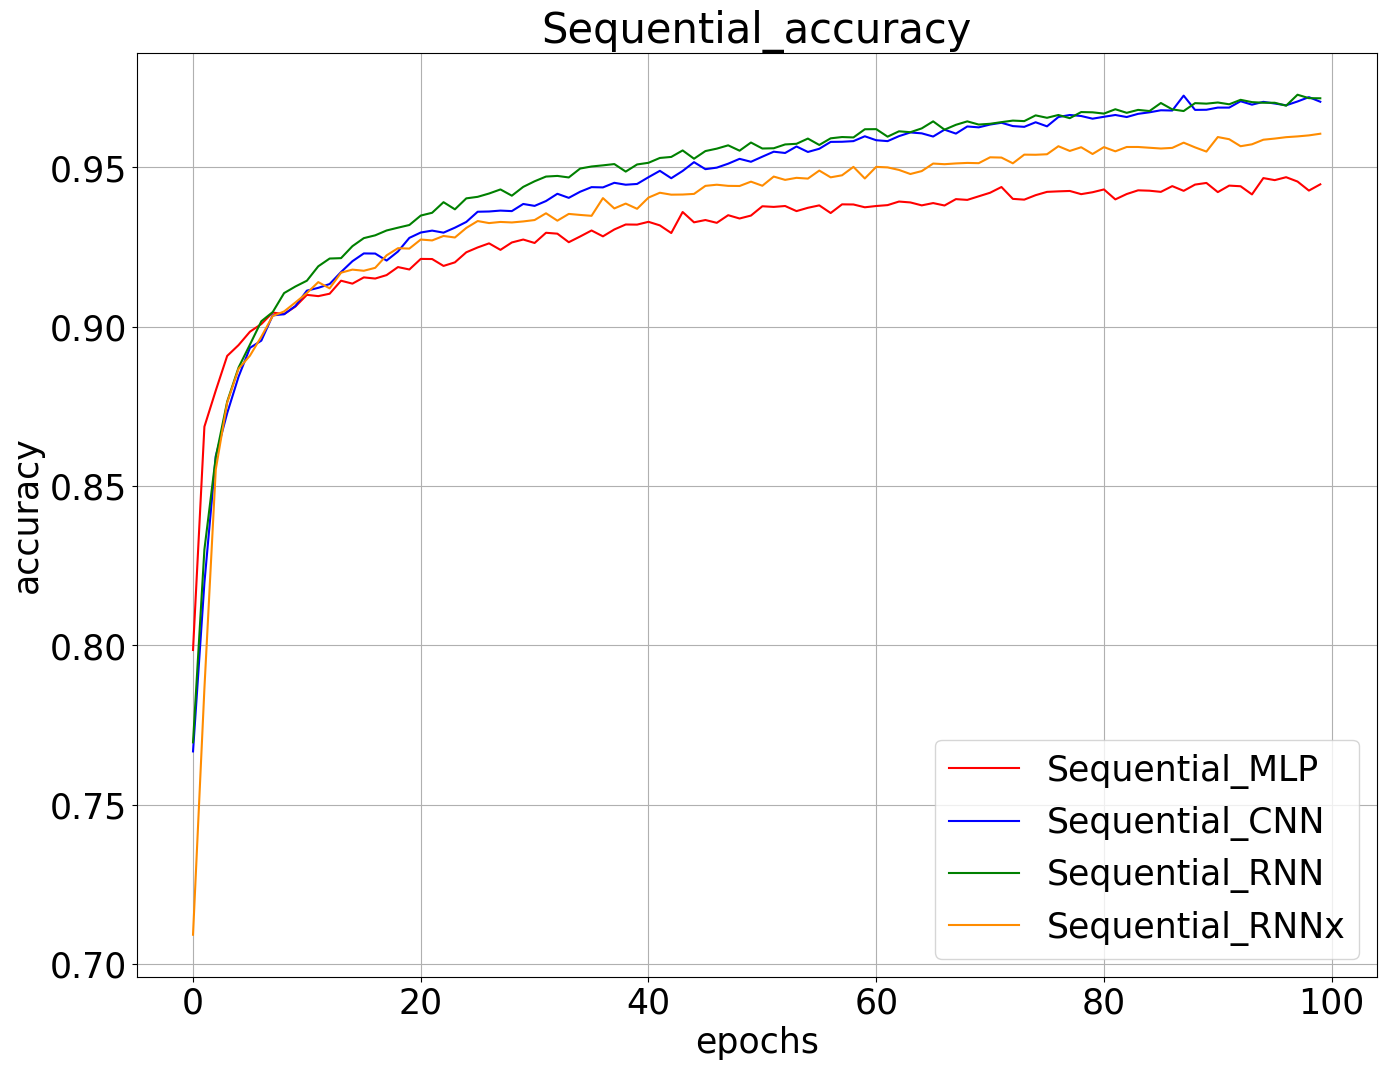
\includegraphics[width=\linewidth]{obrazky-figures/Sequential_experiment/accuracy_2023-03-29_14:45:07.png}
        \caption{Training accuracy progress.}
        \label{graph-sequential-accuracy}
    \end{minipage}\hfill
    \begin{minipage}{0.48\textwidth}
        \centering
        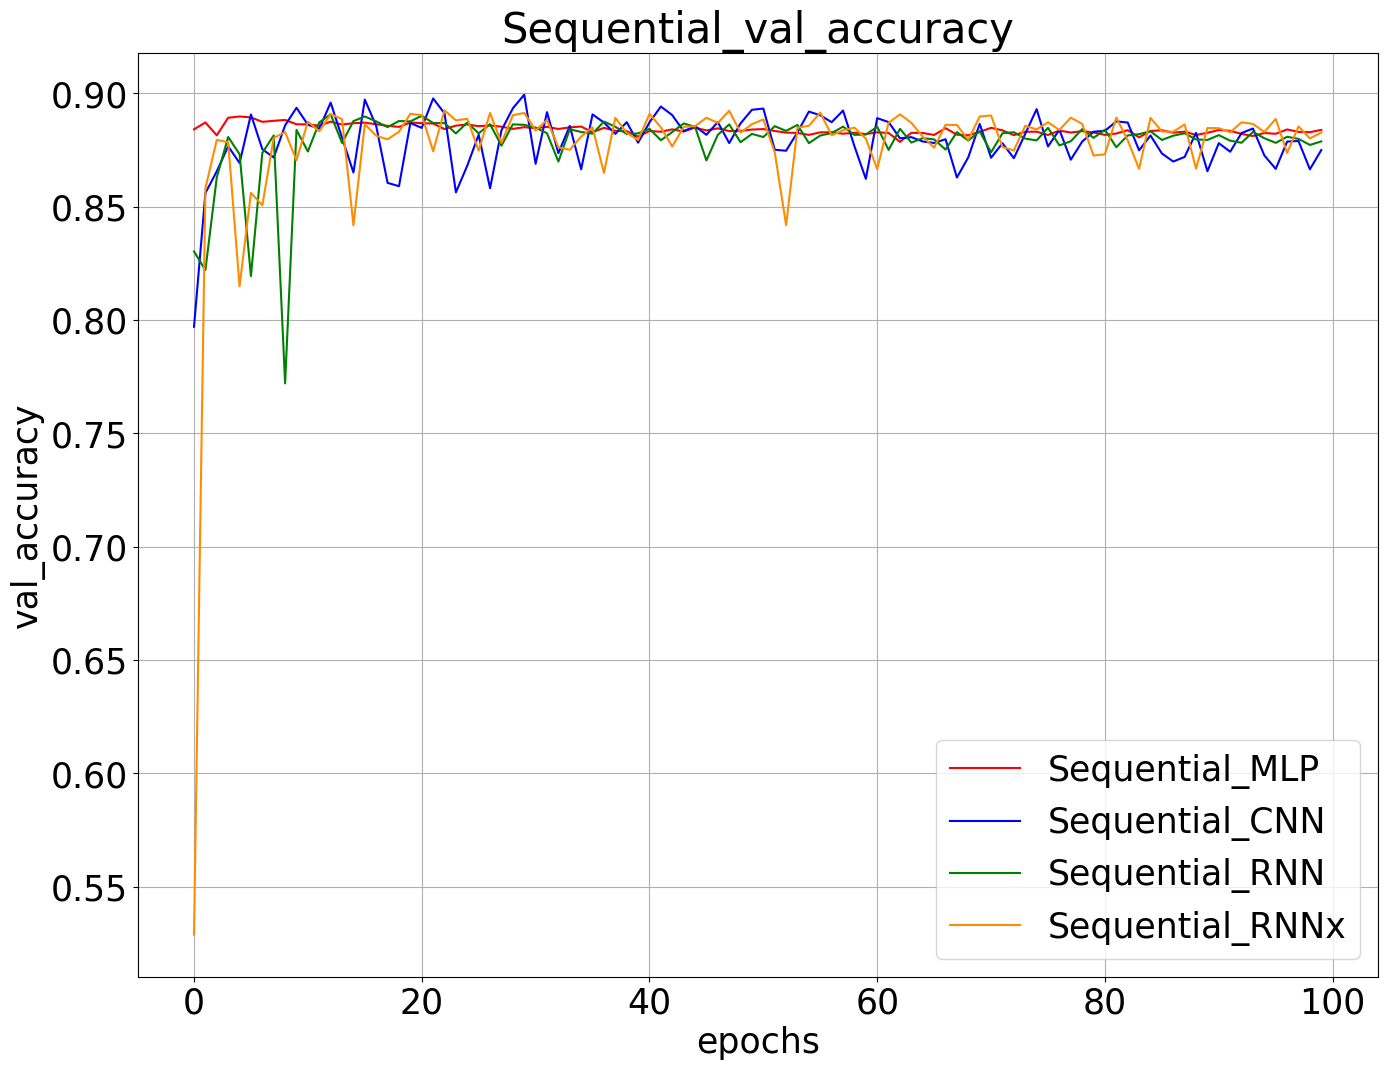
\includegraphics[width=\linewidth]{obrazky-figures/Sequential_experiment/val_accuracy_2023-03-29_14:45:07.png}
        \caption{Validation accuracy progress.}
        \label{graph-sequential-val_accuracy}
    \end{minipage}
\end{figure}
In terms of training accuracy (figure \ref{graph-sequential-accuracy}), the best performing (0.9716, 100th epoch) was
\texttt{Sequential\_RNN}, but \texttt{Sequential\_CNN} kept staying extremely close (0.9706) and based on the curves,
it seems that it maybe could have outran \texttt{Sequential\_CNN} if the training continued.
The worst training accuracy was measured by \texttt{Sequential\_MLP} (0.9446, 100th epoch), but it was still quite good.

All models performed quite similarly in terms of validation accuracy (figure \ref{graph-sequential-val_accuracy}),
although \texttt{Sequential\_RNN}'s and \texttt{Sequential\_MLP}'s graphs are more consistent (less spikes).
During the last epoch, all models measured between 0.875 (\texttt{Sequential\_CNN}) and 0.8839
(\texttt{Sequential\_MLP}) validation accuracy.


\subsubsection{Testing phase}
\begin{figure}[!h]
    \centering
    \begin{minipage}{0.48\textwidth}
        \centering
        \captionsetup{justification=centering}
        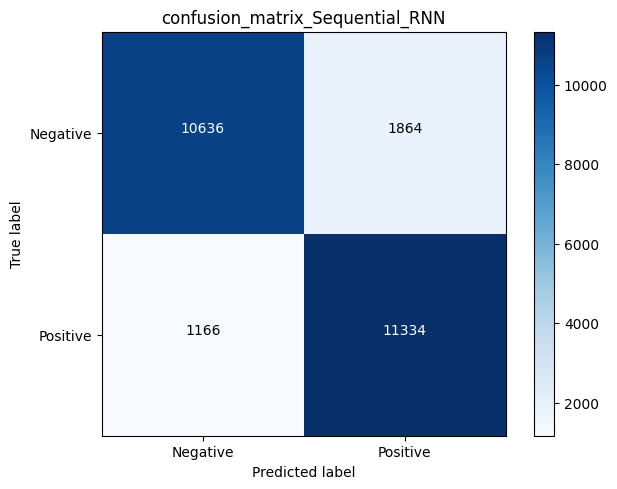
\includegraphics[width=\linewidth]{obrazky-figures/Sequential_experiment/confusion_matrix_Sequential_RNN_2023-04-07_16:57:21.png}
        \caption{Confusion matrix of \texttt{Sequential\_RNN}.}
        \label{graph-sequential-cm-rnn}
    \end{minipage}\hfill
    \begin{minipage}{0.48\textwidth}
        \centering
        \captionsetup{justification=centering}
        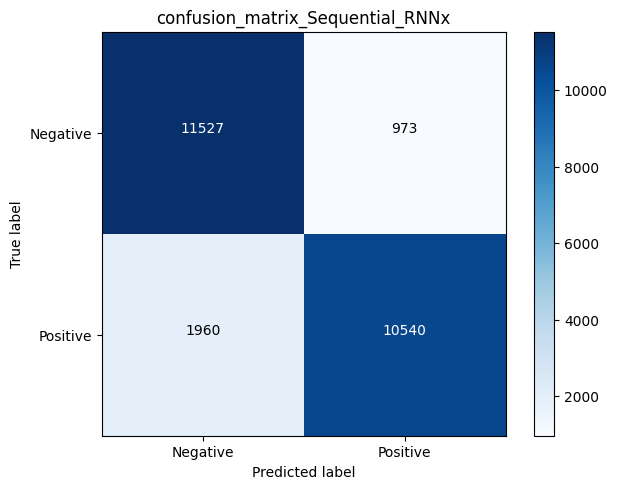
\includegraphics[width=\linewidth]{obrazky-figures/Sequential_experiment/confusion_matrix_Sequential_RNNx_2023-04-07_16:57:33.png}
        \caption{Confusion matrix of \texttt{Sequential\_RNNx}.}
        \label{graph-sequential-cm-rnnx}
    \end{minipage}
\end{figure}
Judging from the confusion matrices, it seems that the recurrent models have developed opposite biases.
While \texttt{Sequential\_RNN} (figure \ref{graph-sequential-cm-rnn}), having only one LSTM-based layer,
is more prone to misclassifying a negative review as positive, the deeper (stacked)\\ \texttt{Sequential\_RNNx}
(\ref{graph-sequential-cm-rnnx}) seems to have an even stronger bias, but this time towards false negatives.


\begin{figure}[!h]
    \centering
    \begin{minipage}{0.48\textwidth}
        \centering
        \captionsetup{justification=centering}
        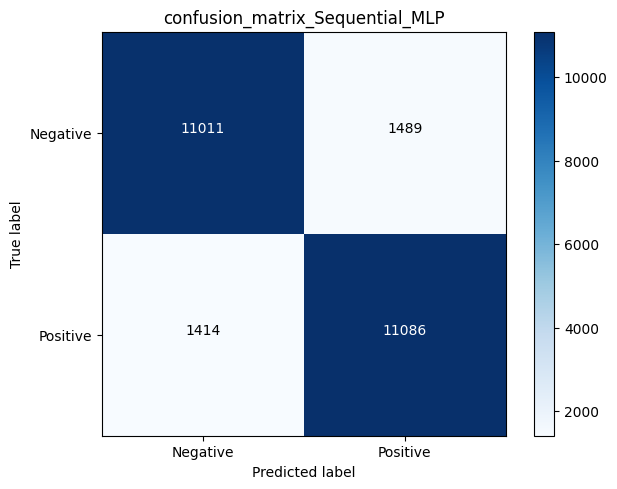
\includegraphics[width=\linewidth]{obrazky-figures/Sequential_experiment/confusion_matrix_Sequential_MLP_2023-04-07_16:57:13.png}
        \caption{Confusion matrix of \texttt{Sequential\_MLP}.}
        \label{graph-sequential-cm-mlp}
    \end{minipage}\hfill
    \begin{minipage}{0.48\textwidth}
        \centering
        \captionsetup{justification=centering}
        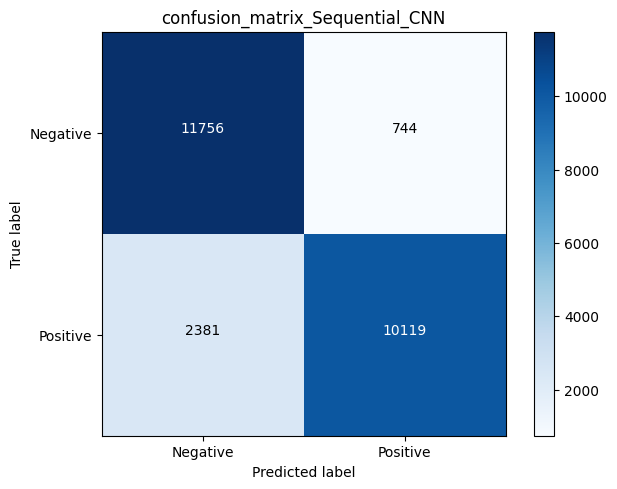
\includegraphics[width=\linewidth]{obrazky-figures/Sequential_experiment/confusion_matrix_Sequential_CNN_2023-04-07_16:57:15.png}
        \caption{Confusion matrix of \texttt{Sequential\_CNN}.}
        \label{graph-sequential-cm-cnn}
    \end{minipage}
\end{figure}
Since the only information available for \texttt{Sequential\_MLP} (figure \ref{graph-sequential-cm-mlp})
is the occurrence (0/1) of each word,
I really expected it to strongly associate certain words with a certain class and build up a strong bias.
The opposite is actually true, as it is surprisingly the least biased model.

On the contrary, \texttt{Sequential\_CNN} (figure \ref{graph-sequential-cm-cnn})
is more than three times as likely to predict a false negative than to
predict a false positive, making it the most biased model of the experiment.


\begin{table}[!h]
\centering
\begin{tabular}{|c|c|c|c|c|}
    \cline{1-5}
    \textbf{Metric} & \texttt{Sequential\_MLP} & \texttt{Sequential\_CNN} & \texttt{Sequential\_RNN} &
    \texttt{Sequential\_RNNx} \\
    \cline{1-5}
    Loss & 0.34997347 & 0.47943094 & 0.45871839 & 0.48976046 \\
    \cline{1-5}
    Accuracy & 0.88388002 & 0.87944001 & 0.87922668 & 0.88009000 \\
    \cline{1-5}
\end{tabular}
\caption{Loss and metrics values measured during the testing phase of the sequential data experiment.}
\label{table:sequential-test}
\end{table}
Table \ref{table:sequential-test} confirms that the performance of \texttt{Sequential\_RNN} and
\texttt{Sequential\_CNN} is roughly the same. \texttt{Sequential\_RNNx} has worse test performance than
\texttt{Sequential\_MLP}, even though it's training performance was not marginally better, which is quite
bad for a recurrent model considering the nature of the experiment (natural language processing).


\subsection{Conclusion}
The convolutional model, \texttt{Sequential\_CNN}, managed to reach the same levels of performance as the better one
of the
recurrent models (\texttt{Sequential\_RNN}), while only having convolutional kernels of size 3. It should
also be mentioned that none of the recurrent models had recurrent dropout (setting some of the ``remembered''
context to zero, instead of the input), as that massively slowed down their training when I experimented with it,
so I decided to only use standard dropouts with very high rates, that could have possibly negatively impacted
the performance of both models.

Comparing the two recurrent models, there was really no criteria by which the stacked \texttt{Sequential\_RNNx}
would beat the ``simpler'' model, so I assume that unless the problem is quite complex, adding additional layers
may have a negative impact, while simply adding more recurrent cells usually shouldn't cause much harm
and should be preferred.

What attracts the most attention is the performance of \texttt{Sequential\_MLP}. It demonstrated
that using less information might be even beneficial in cases where the ocurrence of certain tokens (words)
strongly characterizes the classes. Word embedding could have been used for training this model as well,
in which case each word-vector would be simply interpreted as 32 individual features, but the input
layer would be massively wide and I also wanted to try something different,
which, I suppose, actually paid off.




\section{Summary}
\label{experiment-summary}
It is crucial to realize that comparing the models based solely on performance shouldn't be the only focus,
as there are just too many factors that can influence the results. The models were regularized heavily to
generalize
well, but for example, once model $A$ shows better training performance, but worse validation/test performance
than model $B$, it can imply that model $B$ was just regularized a bit more. One should also focus
on the visible characteristics of the models shown throughout the experiments. 

What the experiments demonstrated very well is that when presented with a problem,
one should not simply choose the ``canonical'' NN type suited for the problem, but also consider
the alternatives based on analyzing the problem first.
The best examples seem to be \texttt{Tabular\_RNN}
from the first experiment and \texttt{Sequential\_CNN} from the third experiment.
The third experiment also demonstrated (through \texttt{Sequential\_MLP}'s performance), that sometimes,
it might be worth to consider a simplification of the data's interpretation, as it might be even beneficial
for dealing with some shortcomings (the class bias in this case).

In summary, usually all models performed fairly well regardless of the type of the problem
(I would consider \texttt{Tabular\_CNN} in the first problem as the worst exception), but keep in mind
that the problems were rather simple, so this trend is not guaranteed to transfer to marginally larger scales
of most modern practical problems, that are often solved by models with complex architectures and 
billions of trainable parameters.




\chapter{Conclusion}
\label{conclusion}
The first goal of the thesis was to introduce classification and artificial neural networks,
preferably to a reader with no prior knowledge of the problematics.
The important classification terminology and metrics, understanding of which is crucial for understanding the rest of the work,
were explained clearly, and also some other common classification algorithms were briefly introduced.
Artificial neural networks were explained very gradually, starting from a single neuron, all the way to the
three main ANN types. Modern architectural advancements (e.g. transformers) were either left out completely or
just very briefly mentioned, to really focus on the understanding of the fundamentals.

The second goal was to introduce Keras in the context of classification with ANNs.
The given section was very practically focused, and ordered in the same way a user would approach when building
a classification model. The code snippets often purposely demonstrated different ways of performing a certain action,
and while some parts of the text might seem overfilled with Keras' diverse options (loss, metrics, etc.),
those options were introduced practically, to guide the reader's choices when building his own models.

The third and last goal was to perform experiments showing the differences between the three main ANN types.
Since the original ideas for the experiments were lacking in many aspects, there was a need for a way to compare
all three ANN types on a problem, that unbiasedly favors none of them. This was solved by performing an individual
experiment for each of the corresponding data types, and the requirement for comparing different ANN topologies was met
by always introducing an additional ANN of the given type. The preparation of the experiments was crucial in this case,
and all choices, including selecting the number of trainable parameters as the performance-similarity benchmark,
were backed up by an explanation. The experimental application is rather simple and focused mainly on its main purpose,
but also provides many utilities for a smooth practical usage.

Even though a straight performance comparison of different ANN types is almost impossible, since there are simply
too many factors having possibly detrimental effects on the results to consider, the experiments demonstrated
the usefulness of the individual ANN types on problems where they may have not been considered normally.
Some interesting, unexpected findings emerged throughout the course of the experiments too.

A very appropriate way of extending this work might be a continuation focusing on modern ANN architectures
and even on specific models, possibly with an emphasis on generative models, which have been rapidly gaining popularity
by the time of finishing this thesis. This could also incorporate inventing some creative ways of comparing
such models.
Some other possibilities include comparing different classification algorithms (not only ANNs) or extending
the work to a different problem domain (e.g. regression), but today's circumstances create many great opportunities
favoring the first approach.










%The preparation of the experiments was a very crucial part in this case. It had been described in detail,
%and all the crucial choices were backed up by an explanation. The description of the experimental application
%was very brief, to not distract the reader from the experiments too much.

%=========================================================================

  \else
    \input{projekt-01-kapitoly-chapters}
  \fi
  
  % Kompilace po částech (viz výše, nutno odkomentovat)
  % Compilation piecewise (see above, it is necessary to uncomment it)
  %\subfile{projekt-01-uvod-introduction}
  % ...
  %\subfile{chapters/projekt-05-conclusion}


  % Pouzita literatura / Bibliography
  % ----------------------------------------------
\ifslovak
  \makeatletter
  \def\@openbib@code{\addcontentsline{toc}{chapter}{Literatúra}}
  \makeatother
  \bibliographystyle{bib-styles/Pysny/skplain}
\else
  \ifczech
    \makeatletter
    \def\@openbib@code{\addcontentsline{toc}{chapter}{Literatura}}
    \makeatother
    \bibliographystyle{bib-styles/Pysny/czplain}
  \else 
    \makeatletter
    \def\@openbib@code{\addcontentsline{toc}{chapter}{Bibliography}}
    \makeatother
    \bibliographystyle{bib-styles/Pysny/enplain}
  %  \bibliographystyle{alpha}
  \fi
\fi
  \begin{flushleft}
  \bibliography{projekt-20-literatura-bibliography}
  \end{flushleft}

  % vynechani stranky v oboustrannem rezimu
  % Skip the page in the two-sided mode
  \iftwoside
    \cleardoublepage
  \fi

  % Prilohy / Appendices
  % ---------------------------------------------
  \appendix
\ifczech
  \renewcommand{\appendixpagename}{Přílohy}
  \renewcommand{\appendixtocname}{Přílohy}
  \renewcommand{\appendixname}{Příloha}
\fi
\ifslovak
  \renewcommand{\appendixpagename}{Prílohy}
  \renewcommand{\appendixtocname}{Prílohy}
  \renewcommand{\appendixname}{Príloha}
\fi
%  \appendixpage

% vynechani stranky v oboustrannem rezimu
% Skip the page in the two-sided mode
%\iftwoside
%  \cleardoublepage
%\fi
  
\ifslovak
%  \section*{Zoznam príloh}
%  \addcontentsline{toc}{section}{Zoznam príloh}
\else
  \ifczech
%    \section*{Seznam příloh}
%    \addcontentsline{toc}{section}{Seznam příloh}
  \else
%    \section*{List of Appendices}
%    \addcontentsline{toc}{section}{List of Appendices}
  \fi
\fi
  \startcontents[chapters]
  \setlength{\parskip}{0pt} 
  % seznam příloh / list of appendices
  % \printcontents[chapters]{l}{0}{\setcounter{tocdepth}{2}}
  
  \ifODSAZ
    \setlength{\parskip}{0.5\bigskipamount}
  \else
    \setlength{\parskip}{0pt}
  \fi
  
  % vynechani stranky v oboustrannem rezimu
  \iftwoside
    \cleardoublepage
  \fi
  
  % Přílohy / Appendices
  \ifenglish
    \chapter{Contents of the included storage media}
\label{appendix-storage-content}

\begin{itemize}
    \item \texttt{\textbf{/app/}} -- The experimental application (source code, datasets, working directories,  instructions).
    \item \texttt{\textbf{/experiments\_results/}} -- Results of the experiments generated by the experimental application.
    \item \texttt{\textbf{/model\_plots/}} -- Model plots of the neural network architectures used in the experiments.
    \item \texttt{\textbf{/text/}} -- \LaTeX source codes of this thesis.
    \item \texttt{\textbf{xpysik00-thesis.pdf}} -- This thesis in PDF format.
\end{itemize}



\chapter{Model plots of the used neural network architectures}
\label{appendix-plots}

\section{Tabular data - MiniBooNE particle identification}
\begin{figure}[hb!]
    \centering
    \begin{minipage}{0.5\textwidth}
        \centering
        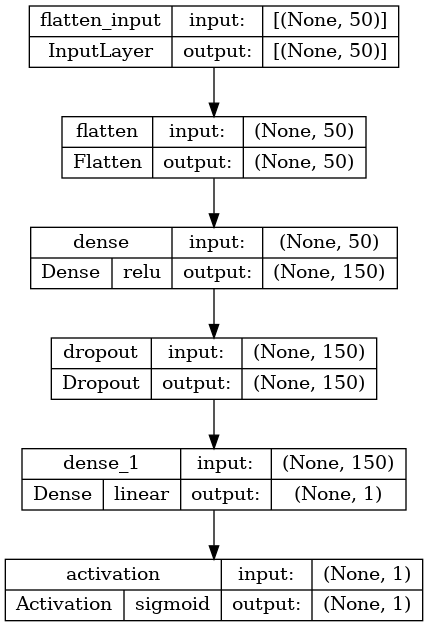
\includegraphics[width=5.3cm]{obrazky-figures/model-plots/Tabular_MLP.png} % first figure itself
        \caption{Tabular\_MLP}
    \end{minipage}\hfill
    \begin{minipage}{0.5\textwidth}
        \centering
        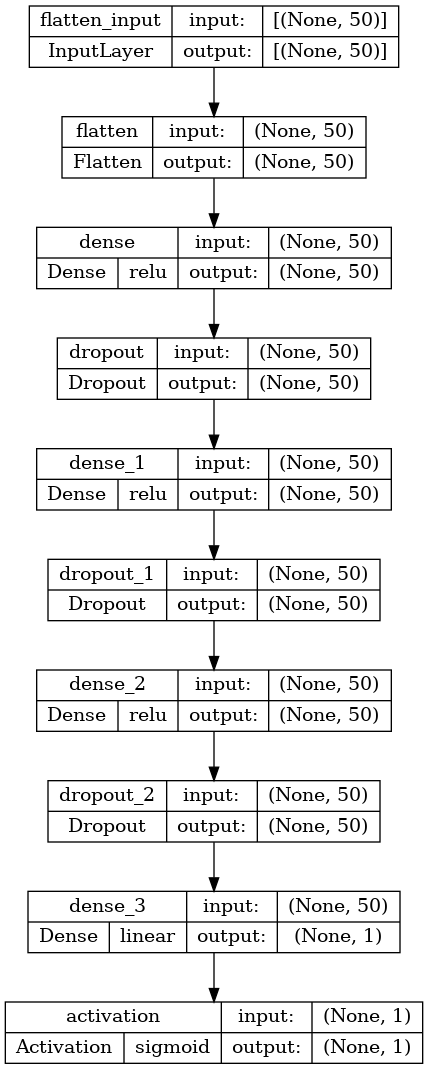
\includegraphics[width=5.3cm]{obrazky-figures/model-plots/Tabular_MLPx.png} % second figure itself
        \caption{Tabular\_MLPx}
    \end{minipage}
\end{figure}
\begin{figure}[!ht]
    \centering
    \begin{minipage}{0.5\textwidth}
        \centering
        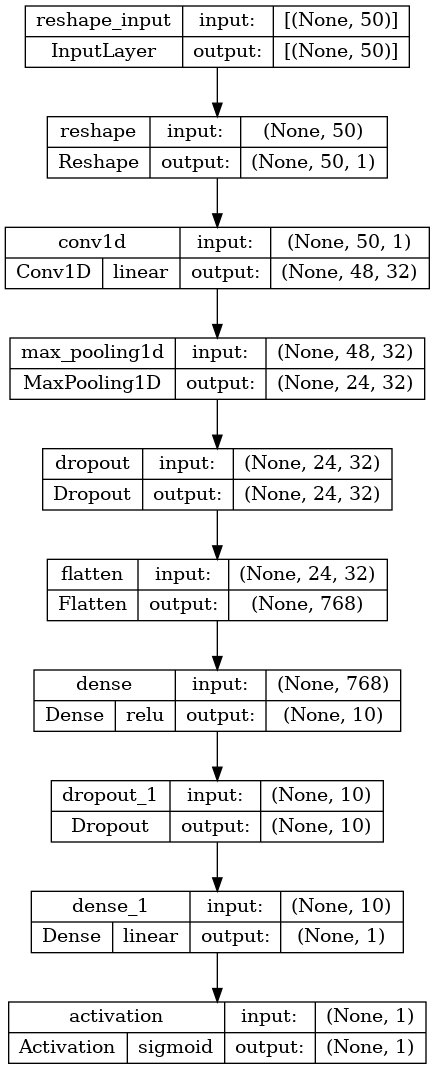
\includegraphics[width=\linewidth]{obrazky-figures/model-plots/Tabular_CNN.png} % first figure itself
        \caption{Tabular\_CNN}
    \end{minipage}\hfill
    \begin{minipage}{0.5\textwidth}
        \centering
        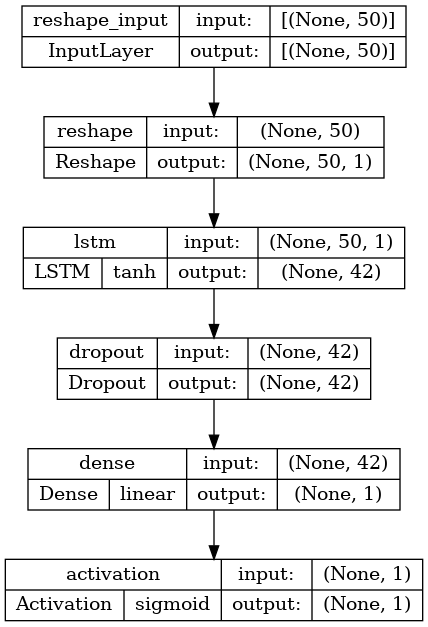
\includegraphics[width=\linewidth]{obrazky-figures/model-plots/Tabular_RNN.png} % second figure itself
        \caption{Tabular\_RNN}
    \end{minipage}
\end{figure}
\newpage

\section{Image data - Fashion-MNIST}
\begin{figure}[!hb]
    \centering
    \begin{minipage}{0.5\textwidth}
        \centering
        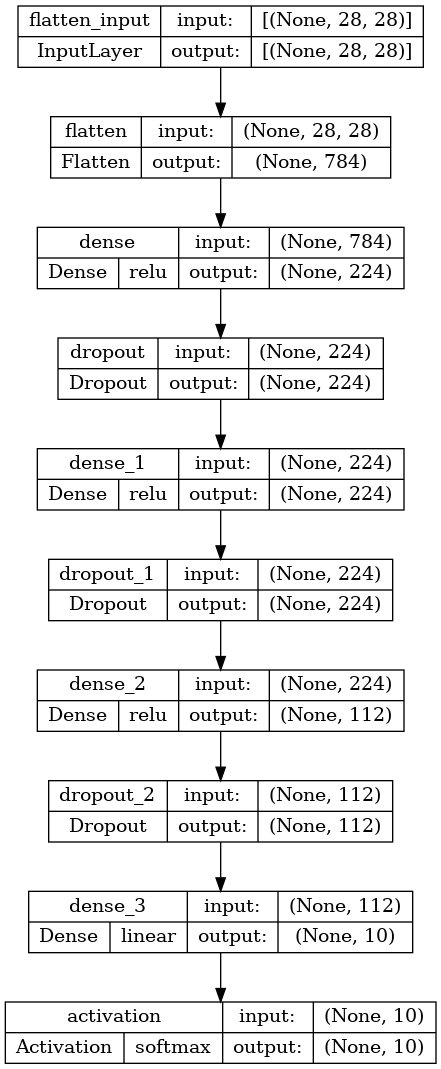
\includegraphics[width=6.2cm]{obrazky-figures/model-plots/Image_MLP.png} % first figure itself
        \caption{Image\_MLP}
    \end{minipage}\hfill
    \begin{minipage}{0.5\textwidth}
        \centering
        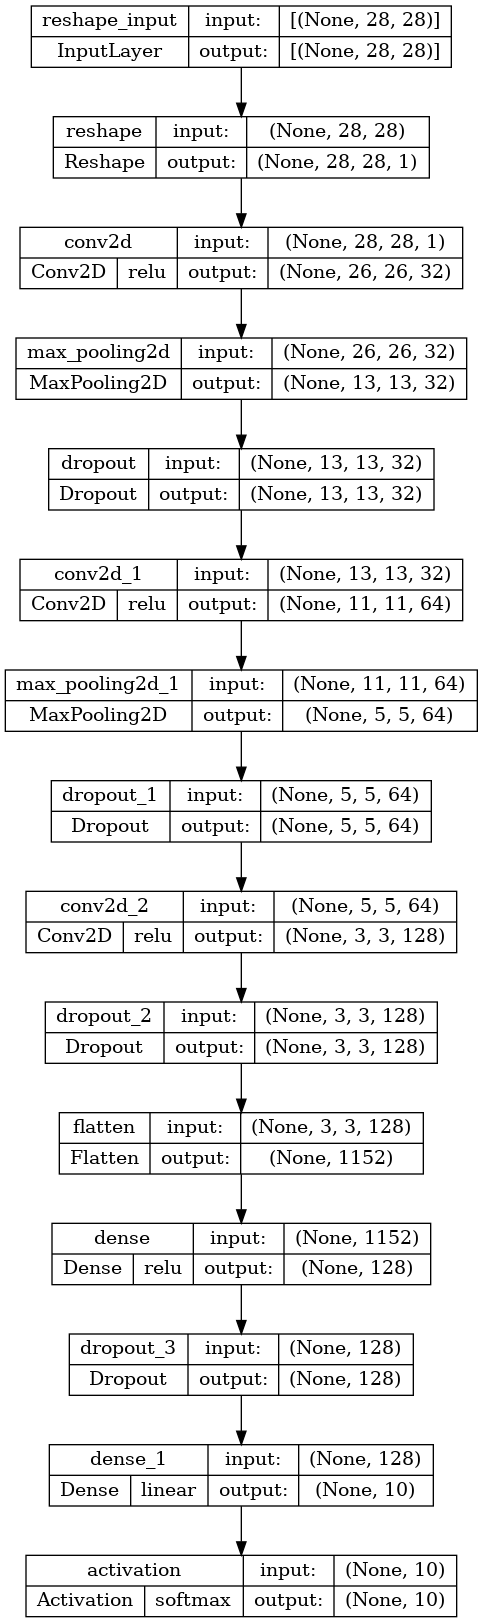
\includegraphics[width=6.2cm]{obrazky-figures/model-plots/Image_CNN.png} % second figure itself
        \caption{Image\_MLPx}
    \end{minipage}
\end{figure}
\begin{figure}[!ht]
    \centering
    \begin{minipage}{0.5\textwidth}
        \centering
        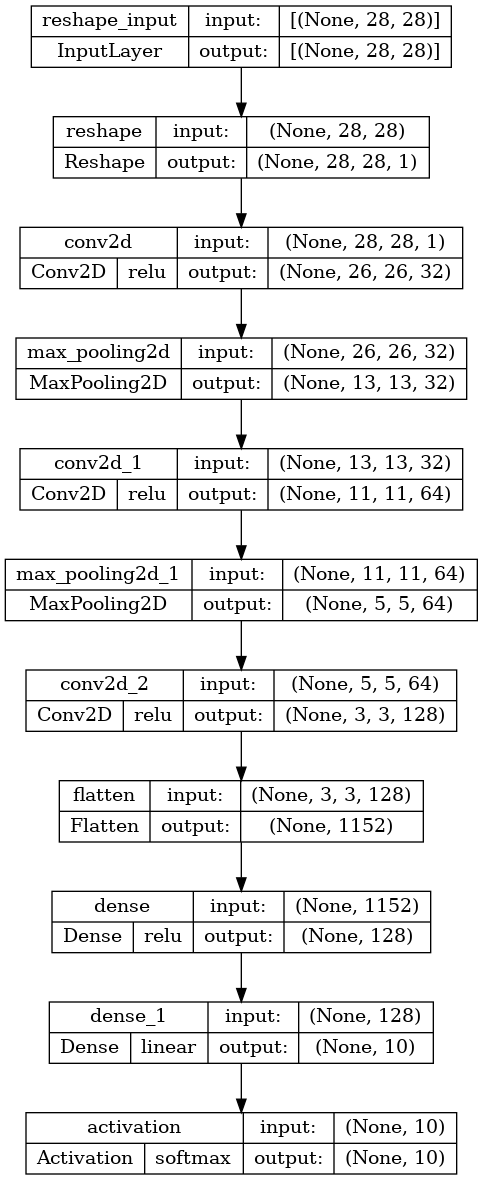
\includegraphics[width=\linewidth]{obrazky-figures/model-plots/Image_CNNx.png} % first figure itself
        \caption{Image\_CNN}
    \end{minipage}\hfill
    \begin{minipage}{0.5\textwidth}
        \centering
        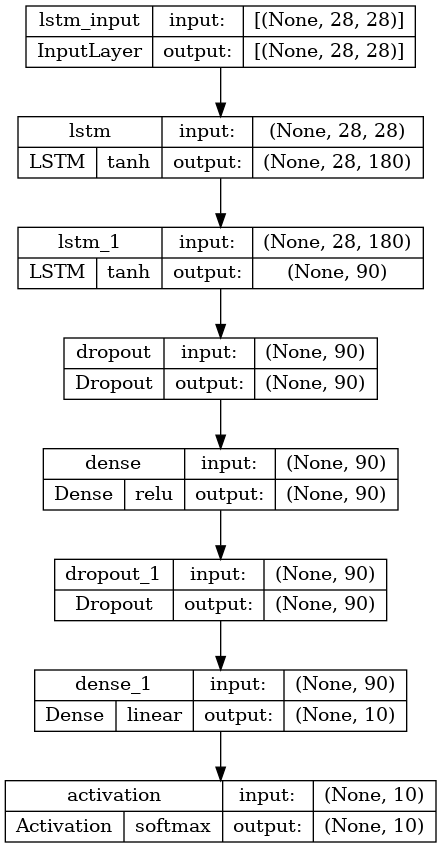
\includegraphics[width=\linewidth]{obrazky-figures/model-plots/Image_RNN.png} % second figure itself
        \caption{Image\_RNN}
    \end{minipage}
\end{figure}
\newpage

\section{Sequential data - IMDB movie review sentiment classification}
\begin{figure}[!hb]
    \centering
    \begin{minipage}{0.5\textwidth}
        \centering
        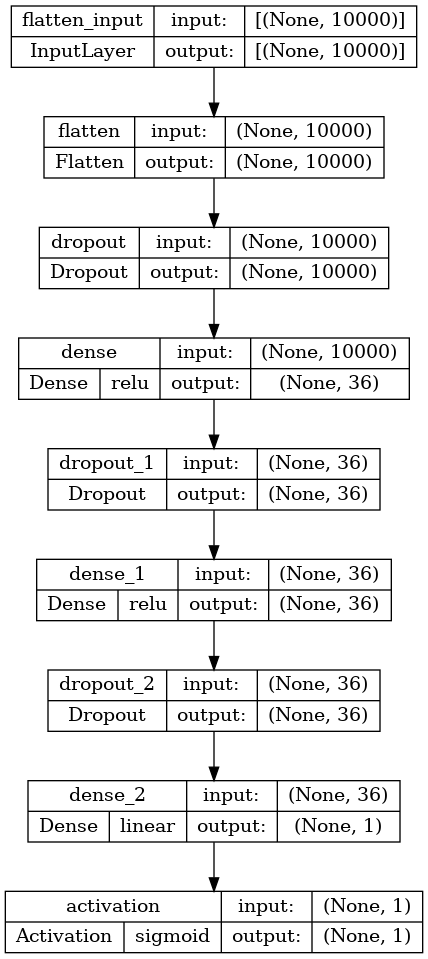
\includegraphics[width=\linewidth]{obrazky-figures/model-plots/Sequential_MLP.png} % first figure itself
        \caption{Sequential\_MLP}
    \end{minipage}\hfill
    \begin{minipage}{0.5\textwidth}
        \centering
        \includegraphics[width=\linewidth]{obrazky-figures/model-plots/Sequential_CNN.png} % second figure itself
        \caption{Sequential\_CNN}
    \end{minipage}
\end{figure}
\begin{figure}[!ht]
    \centering
    \begin{minipage}{0.5\textwidth}
        \centering
        \includegraphics[width=\linewidth]{obrazky-figures/model-plots/Sequential_RNN.png} % first figure itself
        \caption{Sequential\_RNN}
    \end{minipage}\hfill
    \begin{minipage}{0.5\textwidth}
        \centering
        \includegraphics[width=\linewidth]{obrazky-figures/model-plots/Sequential_RNNx.png} % second figure itself
        \caption{Sequential\_RNNx}
    \end{minipage}
\end{figure}




  \else
    \input{projekt-30-prilohy-appendices}
  \fi
  
  % Kompilace po částech (viz výše, nutno odkomentovat)
  % Compilation piecewise (see above, it is necessary to uncomment it)
  %\subfile{projekt-30-prilohy-appendices}
  
\end{document}
